%# -*- coding: utf-8-unix -*-
%% ==================================================
%% File:   final.tex
%% Author: YU Zehan
%% Date:   2018.05.26
%%==================================================

% 论文答辩通过之后,正式归档论文按以下顺序装订:
% === 毕业设计(论文)封皮、内封面、任务书、学术诚信声明、版权使用授权书
% === 中英文摘要: 
% === 目录
% === 正文
% ------- 差分功耗攻击(旁路攻击)的背景知识
% ------- 祖冲之算法的流程
% ------- 对算法的攻击思路
% ------- 实验结果
% ------- 代码分析
%%% 参考文献
%%% (附录)
%%% 谢辞
%%% 英文大摘要


%%==================================================

% 子图

% 双面打印
% \documentclass[bache, openright, twoside]{sjtuthesis}
\documentclass[bachelor, openany, oneside]{sjtuthesis}
% \documentclass[master, review]{sjtuthesis}
% \documentclass[%
%   bachelor|master|doctor, % 必选项
%   fontset=fandol|windows|mac|ubuntu|adobe|founder, % 字体选项
%   oneside|twoside,        % 单面打印,双面打印(奇偶页交换页边距,默认)
%   openany|openright,      % 可以在奇数或者偶数页开新章|只在奇数页开新章(默认)
%   english,                % 启用英文模版
%   review,     % 盲审论文,隐去作者姓名、学号、导师姓名、致谢、发表论文和参与的项目
%   submit      % 定稿提交的论文,插入签名扫描版的原创性声明、授权声明 
% ]

\usepackage{url}
\urlstyle{same}

% 逐个导入参考文献数据库
\addbibresource{bib/final.bib}
% \bibliographystyle{plain}
% \bibliography{bib/final.bib}

\begin{document}

% 无编号内容:中英文论文封面、授权页
%# -*- coding: utf-8-unix -*-
\title{针对祖冲之密码算法电路的差分功耗分析技术研究}
% 序列密码算法电路的新型物理攻防技术研究
% 祖冲之加密算法的差分功耗分析攻击
\author{于泽汉}
\advisor{郭筝}
% \coadvisor{某某教授}
% \defenddate{2018年5月31日}
\school{上海交通大学}
\institute{电子信息与电气工程学院}
\studentnumber{5142119010}
\major{微电子科学与工程}

\englishtitle{A STUDY ON DIFFERENTIAL POWER ANALYSIS OF CIRCUITS RUNNING STREAM CIPHER ALGORITHM}
% A STUDY ON NEW PHYSICAL ATTACKS AND DEFENCES OF CIRCUITS RUNNING STREAM CIPHER ALGORITHM
% AN IMPLEMENTATION OF DIFFERENTIAL POWER ANALYSIS ATTACK ON ZUC ALGORITHM
\englishauthor{\textsc{YU Zehan}}
\englishadvisor{\textsc{GUO Zheng}}
% \englishcoadvisor{Prof. \textsc{Uom Uom}}
\englishschool{Shanghai Jiao Tong University}
\englishinstitute{\textsc{Depart of Micro/Nano Electronics, School of Electronic Infomation and Electrical Engineering} \\
  \textsc{Shanghai Jiao Tong University} \\
  \textsc{Shanghai, P.R.China}}
\englishmajor{Microelectronics}
% \englishdate{May. 31th, 2018}


\maketitle

\makeatletter
\ifsjtu@submit\relax
  % 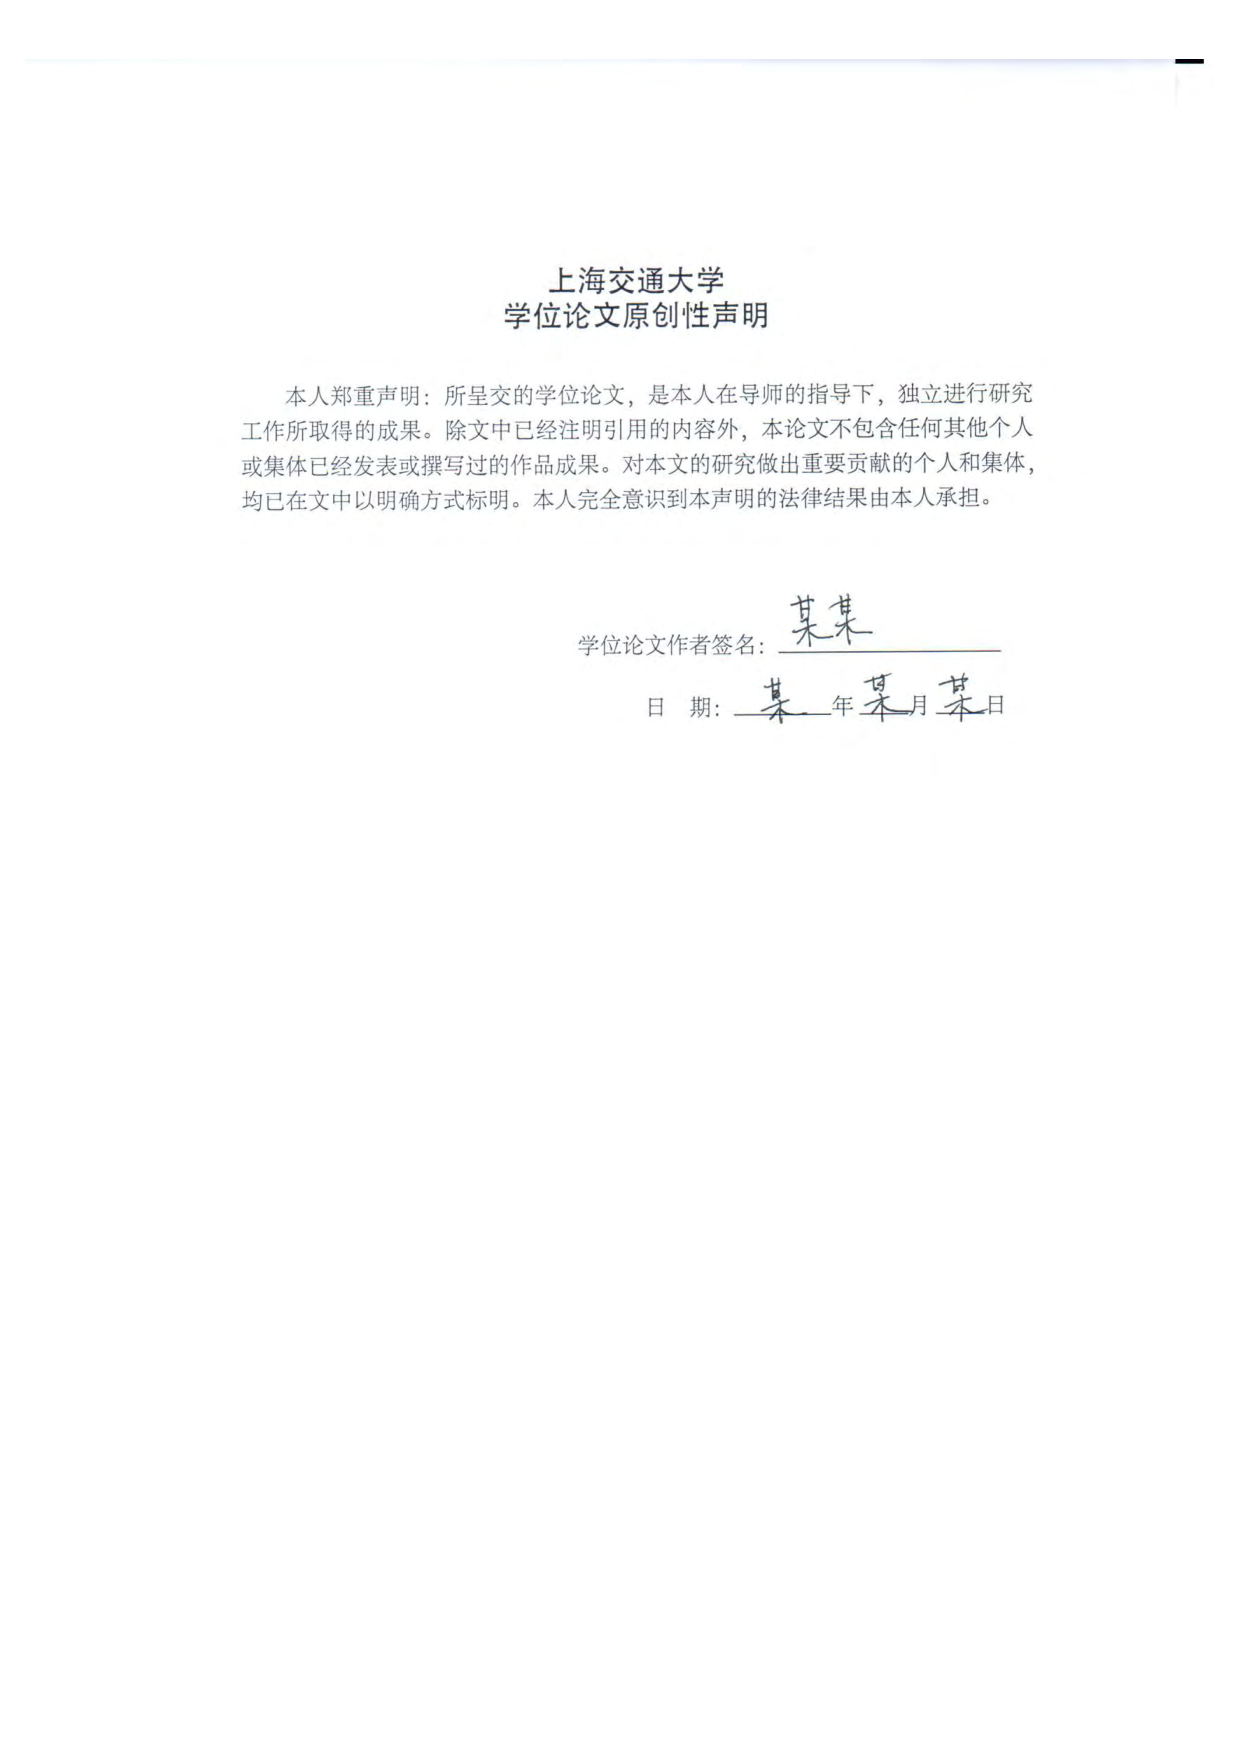
\includepdf{pdf/original.pdf}      % 原创性声明(图片)
  % \cleardoublepage
  % 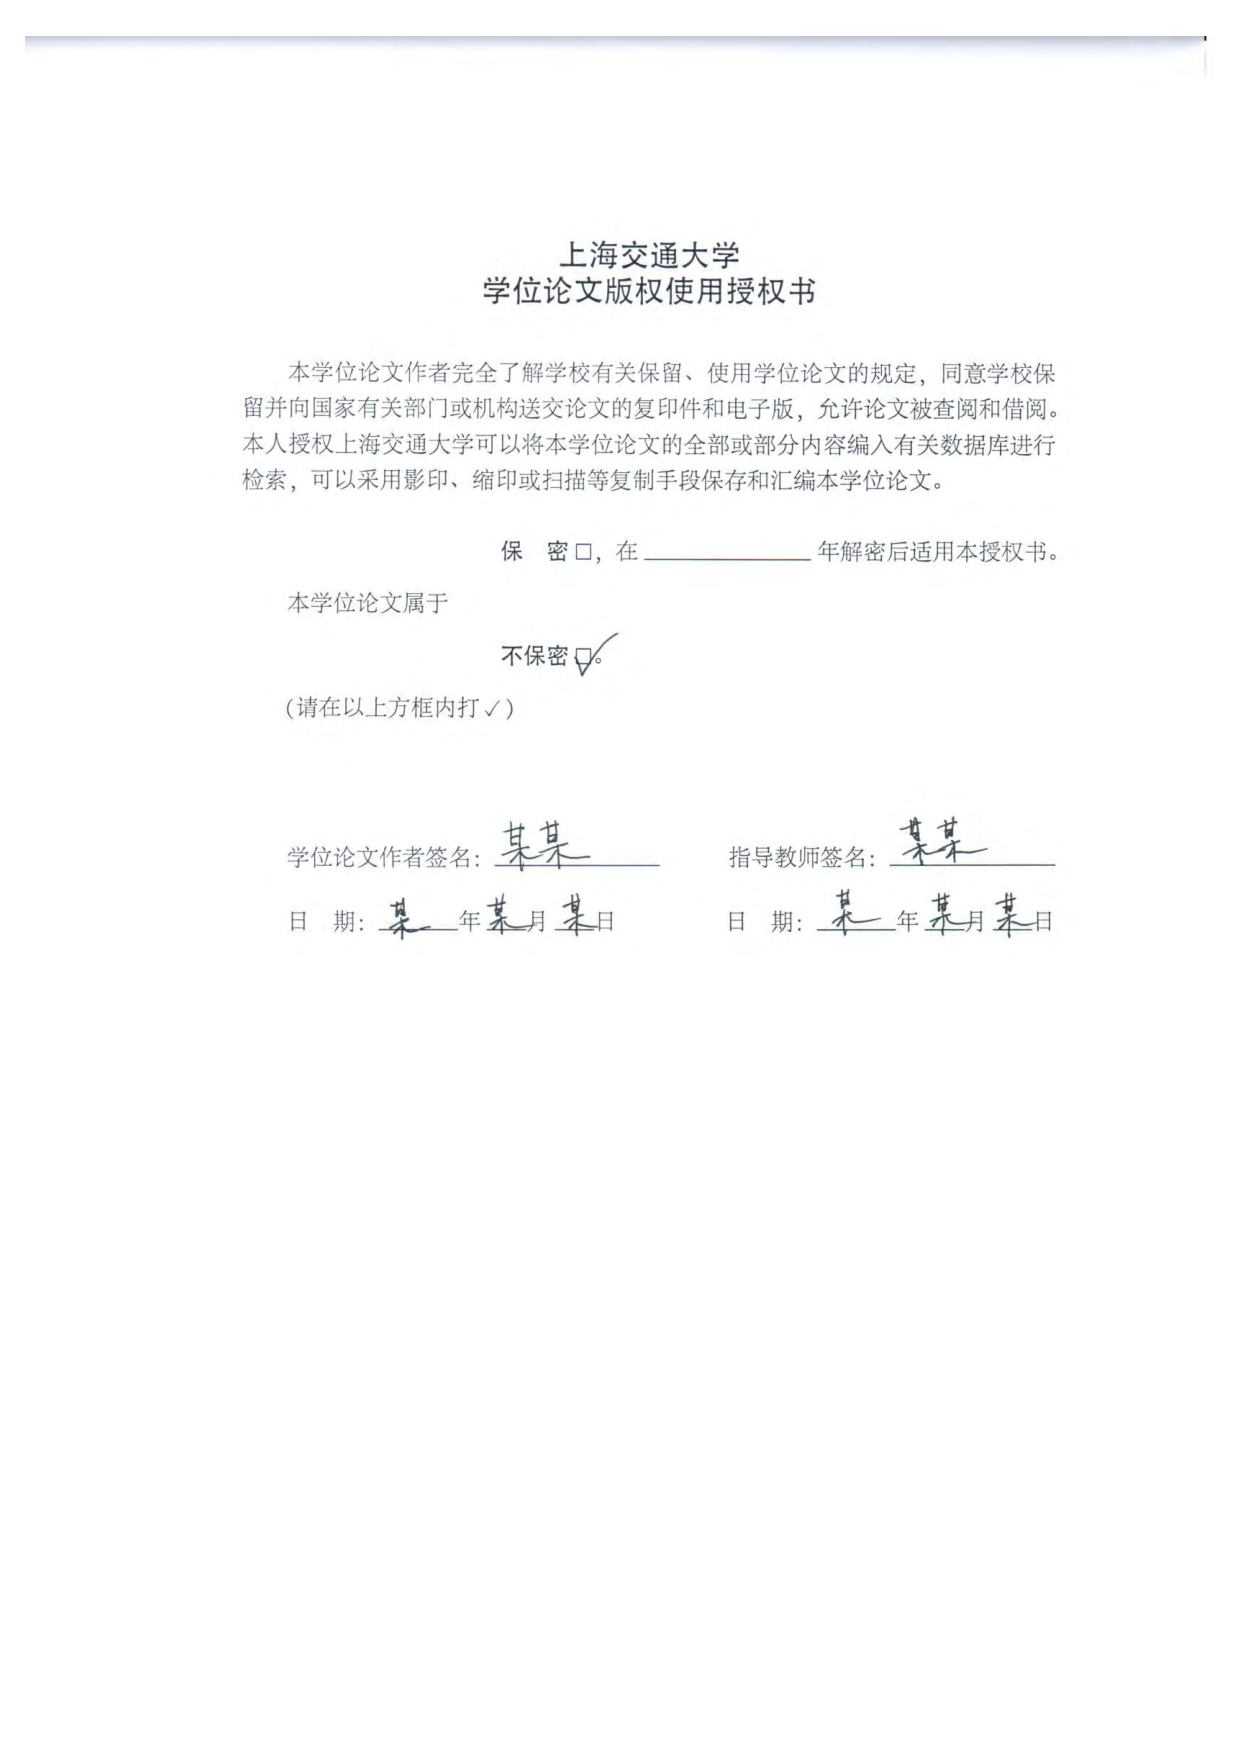
\includepdf{pdf/authorization.pdf} % 授权声明(图片)
  % \cleardoublepage
\else
\ifsjtu@review\relax
% exclude the original claim and authorization
\else
  % \makeDeclareOriginal       % 原创性声明(文本)
  % \makeDeclareAuthorization  % 授权声明  (文本)
\fi
\fi
\makeatother

\frontmatter % 使用罗马数字对前言编号

% 摘要
%# -*- coding: utf-8-unix -*-
%%==================================================
%% 00_abstract.tex
%%==================================================

\begin{abstract}

密码设备的安全性一直备受研究人员关注,其中侧信道攻击技术扮演了十分重要的角色,而功耗分析攻击又是诸多侧信道攻击方法中极为强大的一种。因此,研究功耗分析技术,不但可以加深我们对密码设备安全性的理解,更能揭示出理论安全的密码算法在实际实现时可能会出现的众多问题,从而指导我们在生产实践中采取必要的防护措施。

在传统的旁路攻击中,分组密码是主要的研究对象,这方面的研究成果也较多。由于序列密码(也称为流密码)算法中的加密变换随时间变化,因此,相比分组密码,找到序列密码中密钥和设备功耗之间的对应关系相对困难,所以针对序列密码算法的功耗分析研究相对较少。

本文以祖冲之算法作为序列密码算法的典型,力图将传统的分组密码功耗分析方法应用于序列密码算法,借此表明序列密码算法同样无法抵御功耗分析攻击,并总结出一套系统的模型建立和数据处理的流程和方法。

实验结果显示,通常用于攻击分组密码的差分功耗分析方法也同样适用于祖冲之算法这样的序列密码算法,并且攻击的流程和框架也都基本相同。实验实现了算法的硬件电路和软件代码,成功地攻击出了相关的密钥字节,并且详细分析了算法电路信息泄露的位置,对相关实验结果给出了可能的原因和合理的解释。

\keywords{\large 密码学 \quad 数字电路 \quad 旁路攻击 \quad 差分功耗分析 \quad 祖冲之算法}
\end{abstract}

\begin{englishabstract}
Researchers have paid a lot of attentions to the security of cryptographic devices. Side-channel attacks have greate influences on it. Power analysis is one of the most powerful methods in side-channel attacks. Therefore, the studies on power analysis can not only deepen our understanding of the security of cryptographic devices, but can also reveal a number of potential problems when theoretically secure algorithms are used in real-world applications, which will provide much guidance on the defence of the security of cryptographic devices.

In traditional side-channel attacks, block cipher algorithms are the main objects of study and researchers have a lot of achievements on them. Compared to block cipher algorithms, it is harder for stream cipher algorithms to find the relations between the power of devices and the cipher key of the algorithm for because of the time-variant transformations during encryptions. This leads to less studies on the power analysis of stream cipher algorithms.

This paper studies the technologies used in traditional power analysis of block cipher algorithms, and applies them to stream cipher algorithms. We take the ZUC algorithm as a typical case. The results indicate that stream cipher algorithms are also vulnerable to power analysis attacks. We will build a general process of modeling and data analysis through the experiments.

The experimental results show that the differential power analysis method, which is usually used to attack the block ciphers, also applies to the sequence cipher algorithms such as the ZUC algorithm, and the process and framework of the attack are basically the same. The experiment implements the hardware curcuits and software codes of the algorithm, successfully attacks the related key bytes, and analyzes the location of the information leakage of the algorithm circuit in detail. We also give the possible reasons and reasonable explanations for the related experimental results.

\englishkeywords{\large cryptography, digital circuits, side-channel attack, differential power analysis, ZUC algorithm}
\end{englishabstract}



% 目录、插图目录、表格目录
\tableofcontents
% \listoffigures
% \addcontentsline{toc}{chapter}{\listfigurename}     % 将插图目录加入全文目录
% \listoftables
% \addcontentsline{toc}{chapter}{\listtablename}      % 将表格目录加入全文目录
% \listofalgorithms
% \addcontentsline{toc}{chapter}{\listalgorithmname}  % 将算法目录加入全文目录

% %# -*- coding: utf-8-unix -*-
\begin{nomenclaturename}
\label{chap:symb}

\begin{longtable}{rl}
$\epsilon$     & 介电常数 \\
 $\mu$ 		& 磁导率 \\
 $\epsilon$     & 介电常数 \\
 $\mu$ 		& 磁导率 \\
 $\epsilon$     & 介电常数 \\
 $\mu$ 		& 磁导率 \\
 $\epsilon$ 	& 介电常数 \\
 $\mu$ 		& 磁导率 \\
 $\epsilon$     & 介电常数 \\
 $\mu$ 		& 磁导率 \\
 $\epsilon$     & 介电常数 \\
 $\mu$ 		& 磁导率 \\
 $\epsilon$     & 介电常数 \\
 $\mu$ 		& 磁导率 \\
 $\epsilon$ 	& 介电常数 \\
 $\mu$ 		& 磁导率 \\
 $\epsilon$     & 介电常数 \\
 $\mu$ 		& 磁导率 \\
 $\epsilon$     & 介电常数 \\
 $\mu$ 		& 磁导率 \\
 $\epsilon$     & 介电常数 \\
 $\mu$ 		& 磁导率 \\
 $\epsilon$ 	& 介电常数 \\
 $\mu$ 		& 磁导率 \\
 $\epsilon$     & 介电常数 \\
 $\mu$ 		& 磁导率 \\
 $\epsilon$     & 介电常数 \\
 $\mu$ 		& 磁导率 \\
 $\epsilon$     & 介电常数 \\
 $\mu$ 		& 磁导率 \\
 $\epsilon$ 	& 介电常数 \\
 $\mu$ 		& 磁导率 \\
 $\epsilon$     & 介电常数 \\
 $\mu$ 		& 磁导率 \\
 $\epsilon$     & 介电常数 \\
 $\mu$ 		& 磁导率 \\
 $\epsilon$     & 介电常数 \\
 $\mu$ 		& 磁导率 \\
 $\epsilon$ 	& 介电常数 \\
 $\mu$ 		& 磁导率 \\
 $\epsilon$     & 介电常数 \\
 $\mu$ 		& 磁导率 \\
 $\epsilon$     & 介电常数 \\
 $\mu$ 		& 磁导率 \\
 $\epsilon$     & 介电常数 \\
 $\mu$ 		& 磁导率 \\
 $\epsilon$ 	& 介电常数 \\
 $\mu$ 		& 磁导率 \\
 $\epsilon$     & 介电常数 \\
 $\mu$ 		& 磁导率 \\
 $\epsilon$     & 介电常数 \\
 $\mu$ 		& 磁导率 \\
 $\epsilon$     & 介电常数 \\
 $\mu$ 		& 磁导率 \\
\end{longtable}

\end{nomenclaturename}
 % 主要符号、缩略词对照表

\mainmatter % 使用阿拉伯数字对正文编号

% 正文内容
% %# -*- coding: utf-8-unix -*-
%%==================================================
%% chapter01.tex for SJTU Master Thesis
%%==================================================

%\bibliographystyle{sjtu2}%[此处用于每章都生产参考文献]
\chapter{这是什么}
\label{chap:intro}

这是上海交通大学(非官方)学位论文 \LaTeX 模板,当前版本是 \version 。

最早的一版学位模板是一位热心的物理系同学制作的。
那份模板参考了自动化所学位论文模板,使用了CASthesis.cls文档类,中文字符处理则采用当时最为流行的 \CJKLaTeX 方案。
我根据交大研究生院对学位论文的要求
\footnote{\url{http://www.gs.sjtu.edu.cn/policy/fileShow.ahtml?id=130}}
,结合少量个人审美喜好,完成了一份基本可用的交大 \LaTeX 学位论文模板。
但是,搭建一个 \CJKLaTeX 环境并不简单,单单在Linux下配置环境和添加中文字体,就足够让新手打退堂鼓。
在William Wang的建议下,我开始着手把模板向 \XeTeX 引擎移植。
他完成了最初的移植,多亏了他出色的工作,后续的改善工作也得以顺利进行。

随着我对 \LaTeX 系统认知增加,我又断断续续做了一些完善模板的工作,在原有硕士学位论文模板的基础上完成了交大学士和博士学位论文模板。

现在,交大学位论文模板SJTUTHesis代码在github
\footnote{\url{https://github.com/sjtug/SJTUThesis}}
上维护。
你可以\href{https://github.com/sjtug/SJTUThesis/issues}{在github上开issue}
、或者在\href{https://bbs.sjtu.edu.cn/bbsdoc?board=TeX_LaTeX}{水源LaTeX版}发帖来反映遇到的问题。

\section{使用模板}

\subsection{准备工作}
\label{sec:requirements}

要使用这个模板撰写学位论文,需要在\emph{TeX系统}、\emph{TeX技能}上有所准备。

\begin{itemize}[noitemsep,topsep=0pt,parsep=0pt,partopsep=0pt]
	\item {\TeX}系统:所使用的{\TeX}系统要支持 \XeTeX 引擎,且带有ctex 2.x宏包,以2017年或更新版本的\emph{完整}TeXLive、MacTeX发行版为佳。
	\item TeX技能:尽管提供了对模板的必要说明,但这不是一份“ \LaTeX 入门文档”。在使用前请先通读其他入门文档。
	\item 针对Windows用户的额外需求:学位论文模本分别使用git和GNUMake进行版本控制和构建,建议从Cygwin\footnote{\url{http://cygwin.com}}安装这两个工具。
\end{itemize}

\subsection{模板选项}
\label{sec:thesisoption}

sjtuthesis提供了一些常用选项,在thesis.tex在导入sjtuthesis模板类时,可以组合使用。
这些选项包括:

\begin{itemize}[noitemsep,topsep=0pt,parsep=0pt,partopsep=0pt]
	\item 学位类型:bachelor(学位)、master(硕士)、doctor(博士),是必选项。
	\item 中文字体:fandol(Fandol 开源字体)、windows(Windows 系统下的中文字体)、mac(macOS 系统下的华文字体)、ubuntu(Ubuntu 系统下的文泉驿和文鼎字体)、adobe(Adobe 公司的中文字体)、founder(方正公司的中文字体),默认根据操作系统自动配置。
	\item 英文模版:使用english选项启用英文模版。
	\item 盲审选项:使用review选项后,论文作者、学号、导师姓名、致谢、发表论文和参与项目将被隐去。
\end{itemize}

\subsection{编译模板}
\label{sec:process}

模板默认使用GNUMake构建,GNUMake将调用latemk工具自动完成模板多轮编译:

\begin{lstlisting}[basicstyle=\small\ttfamily, caption={编译模板}, numbers=none]
make clean thesis.pdf
\end{lstlisting}

若需要生成包含“原创性声明扫描件”的学位论文文档,请将扫描件保存为statement.pdf,然后调用make生成submit.pdf。

\begin{lstlisting}[basicstyle=\small\ttfamily, caption={生成用于提交的学位论文}, numbers=none]
make clean submit.pdf
\end{lstlisting}

编译失败时,可以尝试手动逐次编译,定位故障。

\begin{lstlisting}[basicstyle=\small\ttfamily, caption={手动逐次编译}, numbers=none]
xelatex -no-pdf thesis
biber --debug thesis
xelatex thesis
xelatex thesis
\end{lstlisting}

\subsection{模板文件布局}
\label{sec:layout}

\begin{lstlisting}[basicstyle=\small\ttfamily,caption={模板文件布局},label=layout,float,numbers=none]
├── LICENSE
├── Makefile
├── README.md
├── bib
│   ├── chap1.bib
│   └── chap2.bib
├── bst
│   └── GBT7714-2005NLang.bst
├── figure
│   ├── chap2
│   │   ├── sjtulogo.eps
│   │   ├── sjtulogo.jpg
│   │   ├── sjtulogo.pdf
│   │   └── sjtulogo.png
│   └── sjtubanner.png
├── sjtuthesis.cfg
├── sjtuthesis.cls
├── statement.pdf
├── submit.pdf
├── tex
│   ├── abstract.tex
│   ├── ack.tex
│   ├── app_cjk.tex
│   ├── app_eq.tex
│   ├── app_log.tex
│   ├── chapter01.tex
│   ├── chapter02.tex
│   ├── chapter03.tex
│   ├── conclusion.tex
│   ├── id.tex
│   ├── patents.tex
│   ├── projects.tex
│   ├── pub.tex
│   └── symbol.tex
└── thesis.tex
\end{lstlisting}

本节介绍学位论文模板中木要文件和目录的功能。

\subsubsection{格式控制文件}
\label{sec:format}

格式控制文件控制着论文的表现形式,包括sjtuthesis.cfg和sjtuthesis.cls。
其中,“cls”控制论文主体格式,“cfg”为配置文件。

\subsubsection{主控文件thesis.tex}
\label{sec:thesistex}

主控文件thesis.tex的作用就是将你分散在多个文件中的内容“整合”成一篇完整的论文。
使用这个模板撰写学位论文时,你的学位论文内容和素材会被“拆散”到各个文件中:
譬如各章正文、各个附录、各章参考文献等等。
在thesis.tex中通过“include”命令将论文的各个部分包含进来,从而形成一篇结构完成的论文。
对模板定制时引入的宏包,建议放在导言区。

\subsubsection{各章源文件tex}
\label{sec:thesisbody}

这一部分是论文的主体,是以“章”为单位划分的,包括:

\begin{itemize}[noitemsep,topsep=0pt,parsep=0pt,partopsep=0pt]
	\item 中英文摘要(abstract.tex)。前言(frontmatter)的其他部分,中英文封面、原创性声明、授权信息在sjtuthesis.cls中定义,不单独分离为tex文件。
不单独弄成文件。
	\item 正文(mainmatter)——学位论文正文的各章内容,源文件是chapter\emph{xxx}.tex。
	\item 附录(app\emph{xx}.tex)、致谢(thuanks.tex)、攻读学位论文期间发表的学术论文目录(pub.tex)、个人简历(resume.tex)组成正文后的部分(backmatter)。
参考文献列表由bibtex插入,不作为一个单独的文件。
\end{itemize}

\subsubsection{图片文件夹figure}
\label{sec:fig}

figure文件夹放置了需要插入文档中的图片文件(支持PNG/JPG/PDF/EPS格式的图片),可以在按照章节划分子目录。
模板文件中使用\verb|\graphicspath|命令定义了图片存储的顶层目录,在插入图片时,顶层目录名“figure”可省略。

\subsubsection{参考文献数据库bib}
\label{sec:bib}

目前参考文件数据库目录只存放一个参考文件数据库thesis.bib。
关于参考文献引用,可参考第\ref{chap:example}章中的例子。


% %# -*- coding: utf-8-unix -*-
%%==================================================
%% chapter02.tex for SJTU Master Thesis
%% based on CASthesis
%% modified by wei.jianwen@gmail.com
%% Encoding: UTF-8
%%==================================================

\chapter{{\LaTeX} 排版例子}
\label{chap:example}

\section{列表环境}
\label{sec:list}

\subsection{无序列表}
\label{sec:unorderlist}

以下是一个无序列表的例子,列表的每个条目单独分段。

\begin{itemize}
  \item 这是一个无序列表。
  \item 这是一个无序列表。
  \item 这是一个无序列表。
\end{itemize}

使用\verb+itemize*+环境可以创建行内无序列表。
\begin{itemize*}
  \item 这是一个无序列表。
  \item 这是一个无序列表。
  \item 这是一个无序列表。
\end{itemize*}
行内无序列表条目不单独分段,所有内容直接插入在原文的段落中。

\subsection{有序列表}
\label{sec:orderlist}

使用环境\verb+enumerate+和\verb+enumerate*+创建有序列表,
使用方法无序列表类似。

\begin{enumerate}
  \item 这是一个有序列表。
  \item 这是一个有序列表。
  \item 这是一个有序列表。
\end{enumerate}

使用\verb+enumerate*+环境可以创建行内有序列表。
\begin{enumerate*}
  \item 这是一个默认有序列表。
  \item 这是一个默认有序列表。
  \item 这是一个默认有序列表。
\end{enumerate*}
行内有序列表条目不单独分段,所有内容直接插入在原文的段落中。

\subsection{描述型列表}

使用环境\verb+description+可创建带有主题词的列表,条目语法是\verb+\item[主题] 内容+。
\begin{description}
    \item[主题一] 详细内容
    \item[主题二] 详细内容
    \item[主题三] 详细内容 \ldots
\end{description}

\subsection{自定义列表样式}

可以使用\verb+label+参数控制列表的样式,
详细可以参考WikiBooks\footnote{\url{https://en.wikibooks.org/wiki/LaTeX/List_Structures\#Customizing_lists}}。
比如一个自定义样式的行内有序列表
\begin{enumerate*}[label=\itshape\alph*)\upshape]
  \item 这是一个自定义样式有序列表。
  \item 这是一个自定义样式有序列表。
  \item 这是一个自定义样式有序列表。
\end{enumerate*}

\section{数学排版}
\label{sec:matheq}

\subsection{公式排版}
\label{sec:eqformat}

这里有举一个长公式排版的例子,来自\href{http://www.tex.ac.uk/tex-archive/info/math/voss/mathmode/Mathmode.pdf}{《Math mode》}:

\begin {multline}
  \frac {1}{2}\Delta (f_{ij}f^{ij})=
  2\left (\sum _{i<j}\chi _{ij}(\sigma _{i}-
    \sigma _{j}) ^{2}+ f^{ij}\nabla _{j}\nabla _{i}(\Delta f)+\right .\\
  \left .+\nabla _{k}f_{ij}\nabla ^{k}f^{ij}+
    f^{ij}f^{k}\left [2\nabla _{i}R_{jk}-
      \nabla _{k}R_{ij}\right ]\vphantom {\sum _{i<j}}\right )
\end{multline}

\subsection{SI单位}

使用\verb+siunitx+宏包可以方便地输入SI单位制单位,例如\verb+\SI{5}{\um}+可以得到\SI{5}{\um}。

\subsubsection{一个四级标题}
\label{sec:depth4}

这是全文唯一的一个四级标题。在这部分中将演示了mathtools宏包中可伸长符号(箭头、等号的例子)的例子。

\begin{displaymath}
    A \xleftarrow[n=0]{} B \xrightarrow[LongLongLongLong]{n>0} C 
\end{displaymath}

\begin{eqnarray}
  f(x) & \xleftrightarrow[]{A=B}  & B \\
  & \xleftharpoondown[below]{above} & B \nonumber \\
  & \xLeftrightarrow[below]{above} & B
\end{eqnarray}

又如:

\begin{align}
  \label{eq:none}
  & I(X_3;X_4)-I(X_3;X_4\mid{}X_1)-I(X_3;X_4\mid{}X_2) \nonumber \\
  = & [I(X_3;X_4)-I(X_3;X_4\mid{}X_1)]-I(X_3;X_4\mid{}\tilde{X}_2) \\
  = & I(X_1;X_3;X_4)-I(X_3;X_4\mid{}\tilde{X}_2)
\end{align}

\subsection{定理环境}

模板中定义了丰富的定理环境
algo(算法),thm(定理),lem(引理),prop(命题),cor(推论),defn(定义),conj(猜想),exmp(例),rem(注),case(情形),
bthm(断言定理),blem(断言引理),bprop(断言命题),bcor(断言推论)。
amsmath还提供了一个proof(证明)的环境。
这里举一个“定理”和“证明”的例子。
\begin{thm}[留数定理]
\label{thm:res}
  假设$U$是复平面上的一个单连通开子集,$a_1,\ldots,a_n$是复平面上有限个点,$f$是定义在$U\backslash \{a_1,\ldots,a_n\}$上的全纯函数,
  如果$\gamma$是一条把$a_1,\ldots,a_n$包围起来的可求长曲线,但不经过任何一个$a_k$,并且其起点与终点重合,那么:

  \begin{equation}
    \label{eq:res}
    \ointop_{\gamma}f(z)\,\mathrm{d}z = 2\uppi\mathbf{i}\sum^n_{k=1}\mathrm{I}(\gamma,a_k)\mathrm{Res}(f,a_k)
  \end{equation}

  如果$\gamma$是若尔当曲线,那么$\mathrm{I}(\gamma, a_k)=1$,因此:

  \begin{equation}
    \label{eq:resthm}
    \ointop_{\gamma}f(z)\,\mathrm{d}z = 2\uppi\mathbf{i}\sum^n_{k=1}\mathrm{Res}(f,a_k)
  \end{equation}

      % \oint_\gamma f(z)\, dz = 2\pi i \sum_{k=1}^n \mathrm{Res}(f, a_k ). 

  在这里,$\mathrm{Res}(f, a_k)$表示$f$在点$a_k$的留数,$\mathrm{I}(\gamma,a_k)$表示$\gamma$关于点$a_k$的卷绕数。
  卷绕数是一个整数,它描述了曲线$\gamma$绕过点$a_k$的次数。如果$\gamma$依逆时针方向绕着$a_k$移动,卷绕数就是一个正数,
  如果$\gamma$根本不绕过$a_k$,卷绕数就是零。

  定理\ref{thm:res}的证明。
  
  \begin{proof}
    首先,由……

    其次,……

    所以……
  \end{proof}
\end{thm}

上面的公式例子中,有一些细节希望大家注意。微分号d应该使用“直立体”也就是用mathrm包围起来。
并且,微分号和被积函数之间应该有一段小间隔,可以插入\verb+\,+得到。
斜体的$d$通常只作为一般变量。
i,j作为虚数单位时,也应该使用“直立体”为了明显,还加上了粗体,例如\verb+\mathbf{i}+。斜体$i,j$通常用作表示“序号”。
其他字母在表示常量时,也推荐使用“直立体”譬如,圆周率$\uppi$(需要upgreek宏包),自然对数的底$\mathrm{e}$。
不过,我个人觉得斜体的$e$和$\pi$很潇洒,在不至于引起混淆的情况下,我也用这两个字母的斜体表示对应的常量。


\section{向文档中插入图像}
\label{sec:insertimage}

\subsection{支持的图片格式}
\label{sec:imageformat}

\XeTeX 可以很方便地插入PDF、PNG、JPG格式的图片。

插入PNG/JPG的例子如\ref{fig:SRR}所示。
这两个水平并列放置的图共享一个“图标题”(table caption),没有各自的小标题。

\begin{figure}[!htp]
  \centering
  
\includegraphics[width=4cm]{example/sjtulogo.png}
  \hspace{1cm}
  
\includegraphics[width=4cm]{example/sjtulogo.jpg}
  \bicaption[这里将出现在插图索引中]
    {中文题图}
    {English caption}
  \label{fig:SRR}
\end{figure}

这里还有插入EPS图像和PDF图像的例子,如图\ref{fig:epspdf:a}和图\ref{fig:epspdf:b}。这里将EPS和PDF图片作为子图插入,每个子图有自己的小标题。子图标题使用subcaption宏包添加。

\begin{figure}[!htp]
  \centering
  \subcaptionbox{EPS 图像\label{fig:epspdf:a}}[3cm] %标题的长度,超过则会换行,如下一个小图。
    {
\includegraphics[height=2.5cm]{example/sjtulogo.eps}}
  \hspace{4em}
  \subcaptionbox{PDF 图像,注意这个图略矮些。如果标题很长的话,它会自动换行\label{fig:epspdf:b}}
    {
\includegraphics[height=2cm]{sjtulogo.pdf}}
  \bicaption{插入eps和pdf的例子(使用 subcaptionbox 方式)}{An EPS and PDF demo with subcaptionbox}
  \label{fig:pdfeps-subcaptionbox}
\end{figure}

\begin{figure}[!htp]
  \centering
  \begin{subfigure}{2.5cm}
    \centering
    
\includegraphics[height=2.5cm]{example/sjtulogo.eps}
    \caption{EPS 图像}
  \end{subfigure}
  \hspace{4em}
  \begin{subfigure}{0.4\textwidth}
    \centering
    
\includegraphics[height=2cm]{sjtulogo.pdf}
    \caption{PDF 图像,注意这个图略矮些。subfigure中同一行的子图在顶端对齐。}
  \end{subfigure}
  \bicaption{插入eps和pdf的例子(使用 subfigure 方式)}{An EPS and PDF demo with subfigure}
  \label{fig:pdfeps-subfigure}
\end{figure}

更多关于 \LaTeX 插图的例子可以参考\href{http://www.cs.duke.edu/junhu/Graphics3.pdf}{《\LaTeX 插图指南》}。

\subsection{长标题的换行}
\label{sec:longcaption}

图\ref{fig:longcaptionbad}和图\ref{fig:longcaptiongood}都有比较长图标题,通过对比发现,图\ref{fig:longcaptiongood}的换行效果更好一些。
其中使用了minipage环境来限制整个浮动体的宽度。

\begin{figure}[!htp]
  \centering
  
\includegraphics[width=4cm]{sjtubadge.pdf}
  \bicaption[这里将出现在插图索引]
    {上海交通大学是我国历史最悠久的高等学府之一,是教育部直属、教育部与上海市共建的全国重点大学.}
    {Where there is a will, there is a way.}
 \label{fig:longcaptionbad}
\end{figure}

\begin{figure}[!htbp]
  \centering
  \begin{minipage}[b]{0.6\textwidth}
    \centering
    
\includegraphics[width=4cm]{sjtubadge.pdf}
    \bicaption[出现在插图索引中]
      {上海交通大学是我国历史最悠久的高等学府之一,是教育部直属、教育部与上海市共建的全国重点大学.}
      {Where there is a will, there is a way.}
    \label{fig:longcaptiongood}
  \end{minipage}     
\end{figure}

\subsection{绘制流程图}

图\ref{fig:flow_chart}是一张流程图示意。使用tikz环境,搭配四种预定义节点(\verb+startstop+、\verb+process+、\verb+decision+和\verb+io+),可以容易地绘制出流程图。
\begin{figure}[!htp]
    \centering
    \resizebox{6cm}{!}{\begin{tikzpicture}[node distance=2cm]
    \node (pic) [startstop] {待测图片};
    \node (bg) [io, below of=pic] {读取背景};
    \node (pair) [process, below of=bg] {匹配特征点对};
    \node (threshold) [decision, below of=pair, yshift=-0.5cm] {多于阈值};
    \node (clear) [decision, right of=threshold, xshift=3cm] {清晰?};
    \node (capture) [process, right of=pair, xshift=3cm, yshift=0.5cm] {重采};
    \node (matrix_p) [process, below of=threshold, yshift=-0.8cm] {透视变换矩阵};
    \node (matrix_a) [process, right of=matrix_p, xshift=3cm] {仿射变换矩阵};
    \node (reg) [process, below of=matrix_p] {图像修正};
    \node (return) [startstop, below of=reg] {配准结果};
     
    %连接具体形状
    \draw [arrow](pic) -- (bg);
    \draw [arrow](bg) -- (pair);
    \draw [arrow](pair) -- (threshold);

    \draw [arrow](threshold) -- node[anchor=south] {否} (clear);

    \draw [arrow](clear) -- node[anchor=west] {否} (capture);
    \draw [arrow](capture) |- (pic);
    \draw [arrow](clear) -- node[anchor=west] {是} (matrix_a);
    \draw [arrow](matrix_a) |- (reg);

    \draw [arrow](threshold) -- node[anchor=east] {是} (matrix_p);
    \draw [arrow](matrix_p) -- (reg);
    \draw [arrow](reg) -- (return);
\end{tikzpicture}
}
    \bicaption{绘制流程图效果}{Flow chart}
    \label{fig:flow_chart}
\end{figure}
  
\clearpage

\section{表格}
\label{sec:tab}

这一节给出的是一些表格的例子,如表\ref{tab:firstone}所示。

\begin{table}[!hpb]
  \centering
  \bicaption[指向一个表格的表目录索引]
    {一个颇为标准的三线表格\footnotemark[1]}
    {A Table}
  \label{tab:firstone}
  \begin{tabular}{@{}llr@{}} \toprule
    \multicolumn{2}{c}{Item} \\ \cmidrule(r){1-2}
    Animal & Description & Price (\$)\\ \midrule
    Gnat & per gram & 13.65 \\
    & each & 0.01 \\
    Gnu & stuffed & 92.50 \\
    Emu & stuffed & 33.33 \\
    Armadillo & frozen & 8.99 \\ \bottomrule
  \end{tabular}
\end{table}
\footnotetext[1]{这个例子来自\href{http://www.ctan.org/tex-archive/macros/latex/contrib/booktabs/booktabs.pdf}{《Publication quality tables in LATEX》}(booktabs宏包的文档)。这也是一个在表格中使用脚注的例子,请留意与threeparttable实现的效果有何不同。}

下面一个是一个更复杂的表格,用threeparttable实现带有脚注的表格,如表\ref{tab:footnote}。

\begin{table}[!htpb]
  \bicaption[出现在表目录的标题]
    {一个带有脚注的表格的例子}
    {A Table with footnotes}
  \label{tab:footnote}
  \centering
  \begin{threeparttable}[b]
     \begin{tabular}{ccd{4}cccc}
      \toprule
      \multirow{2}{6mm}{total}&\multicolumn{2}{c}{20\tnote{1}} & \multicolumn{2}{c}{40} &  \multicolumn{2}{c}{60}\\
      \cmidrule(lr){2-3}\cmidrule(lr){4-5}\cmidrule(lr){6-7}
      &www & \multicolumn{1}{c}{k} & www & k & www & k \\ % 使用说明符 d 的列会自动进入数学模式,使用 \multicolumn 对文字表头做特殊处理
      \midrule
      &$\underset{(2.12)}{4.22}$ & 120.0140\tnote{2} & 333.15 & 0.0411 & 444.99 & 0.1387 \\
      &168.6123 & 10.86 & 255.37 & 0.0353 & 376.14 & 0.1058 \\
      &6.761    & 0.007 & 235.37 & 0.0267 & 348.66 & 0.1010 \\
      \bottomrule
    \end{tabular}
    \begin{tablenotes}
    \item [1] the first note.% or \item [a]
    \item [2] the second note.% or \item [b]
    \end{tablenotes}
  \end{threeparttable}
\end{table}

\section{参考文献管理}

 \LaTeX 具有将参考文献内容和表现形式分开管理的能力,涉及三个要素:参考文献数据库、参考文献引用格式、在正文中引用参考文献。
这样的流程需要多次编译:

\begin{enumerate}[noitemsep,topsep=0pt,parsep=0pt,partopsep=0pt]
	\item 用户将论文中需要引用的参考文献条目,录入纯文本数据库文件(bib文件)。
	\item 调用xelatex对论文模板做第一次编译,扫描文中引用的参考文献,生成参考文献入口文件(aux)文件。
	\item 调用bibtex,以参考文献格式和入口文件为输入,生成格式化以后的参考文献条目文件(bib)。
	\item 再次调用xelatex编译模板,将格式化以后的参考文献条目插入正文。
\end{enumerate}

参考文献数据库(thesis.bib)的条目,可以从Google Scholar搜索引擎\footnote{\url{https://scholar.google.com}}、CiteSeerX搜索引擎\footnote{\url{http://citeseerx.ist.psu.edu}}中查找,文献管理软件Papers\footnote{\url{http://papersapp.com}}、Mendeley\footnote{\url{http://www.mendeley.com}}、JabRef\footnote{\url{http://jabref.sourceforge.net}}也能够输出条目信息。

下面是在Google Scholar上搜索到的一条文献信息,格式是纯文本:

\begin{lstlisting}[caption={从Google Scholar找到的参考文献条目}, label=googlescholar, escapeinside="", numbers=none]
    @phdthesis{"白2008信用风险传染模型和信用衍生品的定价",
      title={"信用风险传染模型和信用衍生品的定价"},
      author={"白云芬"},
      year={2008},
      school={"上海交通大学"}
    } 
\end{lstlisting}

推荐修改后在bib文件中的内容为:

\begin{lstlisting}[caption={修改后的参考文献条目}, label=itemok, escapeinside="", numbers=none]
  @phdthesis{bai2008,
    title={"信用风险传染模型和信用衍生品的定价"},
    author={"白云芬"},
    date={2008},
    address={"上海"},
    school={"上海交通大学"}
  } 
\end{lstlisting}

按照教务处的要求,参考文献外观应符合国标GBT7714的要求\footnote{\url{http://www.cces.net.cn/guild/sites/tmxb/Files/19798_2.pdf}}。
在模板中,表现形式的控制逻辑通过biblatex-gb7714-2015包实现\footnote{\url{https://www.ctan.org/pkg/biblatex-gb7714-2015}},基于{Bib\LaTeX}管理文献。在目前的多数TeX发行版中,可能都没有默认包含biblatex-gb7714-2015,需要手动安装。

正文中引用参考文献时,用\verb+\cite{key1,key2,key3...}+可以产生“上标引用的参考文献”,
如\cite{Meta_CN,chen2007act,DPMG}。
使用\verb+\parencite{key1,key2,key3...}+则可以产生水平引用的参考文献,例如\parencite{JohnD,zhubajie,IEEE-1363}。
请看下面的例子,将会穿插使用水平的和上标的参考文献:关于书的\parencite{Meta_CN,JohnD,IEEE-1363},关于期刊的\cite{chen2007act,chen2007ewi},
会议论文\parencite{DPMG,kocher99,cnproceed},
硕士学位论文\parencite{zhubajie,metamori2004},博士学位论文\cite{shaheshang,FistSystem01,bai2008},标准文件\parencite{IEEE-1363},技术报告\cite{NPB2},电子文献\parencite{xiaoyu2001, CHRISTINE1998},用户手册\parencite{RManual}。

总结一些注意事项:
\begin{itemize}
\item 参考文献只有在正文中被引用了,才会在最后的参考文献列表中出现;
\item 参考文献“数据库文件”bib是纯文本文件,请使用UTF-8编码,不要使用GBK编码;
\item 参考文献条目中默认通过date域输入时间。兼容使用year域时会产生编译warning,可忽略。
\end{itemize}

\section{用listings插入源代码}

原先ctexbook文档类和listings宏包配合使用时,代码在换页时会出现莫名其妙的错误,后来经高人指点,顺利解决了。
感兴趣的话,可以看看\href{http://bbs.ctex.org/viewthread.php?tid=53451}{这里}。
这里给使用listings宏包插入源代码的例子,这里是一段C代码。
另外,listings宏包真可谓博大精深,可以实现各种复杂、漂亮的效果,想要进一步学习的同学,可以参考
\href{http://mirror.ctan.org/macros/latex/contrib/listings/listings.pdf}{listings宏包手册}。

\begin{lstlisting}[language={C}, caption={一段C源代码}]
#include <stdio.h>
#include <unistd.h>
#include <sys/types.h>
#include <sys/wait.h>

int main() {
  pid_t pid;

  switch ((pid = fork())) {
  case -1:
    printf("fork failed\n");
    break;
  case 0:
    /* child calls exec */
    execl("/bin/ls", "ls", "-l", (char*)0);
    printf("execl failed\n");
    break;
  default:
    /* parent uses wait to suspend execution until child finishes */
    wait((int*)0);
    printf("is completed\n");
    break;
  }

  return 0;
}
\end{lstlisting}

\section{用algorithm和algorithmicx宏包插入算法描述}

algorithmicx 比 algorithmic 增加了一些命令。
示例如算法\ref{algo:sum_100}和算法\ref{algo:merge_sort},
后者的代码来自\href{http://hustsxh.is-programmer.com/posts/38801.html}{xhSong的博客}。
algorithmicx的详细使用方法见\href{http://mirror.hust.edu.cn/CTAN/macros/latex/contrib/algorithmicx/algorithmicx.pdf}{官方README}。
使用算法宏包时,算法出现的位置很多时候不按照tex文件里的书写顺序, 
需要强制定位时可以使用\verb+\begin{algorithm}[H]+
\footnote{http://tex.stackexchange.com/questions/165021/fixing-the-location-of-the-appearance-in-algorithmicx-environment}

这是写在算法\ref{algo:sum_100}前面的一段话,在生成的文件里它会出现在算法\ref{algo:sum_100}前面。

\begin{algorithm}
% \begin{algorithm}[H] % 强制定位
\caption{求100以内的整数和}
\label{algo:sum_100}
\begin{algorithmic}[1] %每行显示行号
\Ensure 100以内的整数和 % 输出
\State $sum \gets 0$
\For{$i = 0 \to 100$}
    \State $sum \gets sum + i$
  \EndFor
\end{algorithmic}
\end{algorithm}

这是写在两个算法中间的一段话,当算法\ref{algo:sum_100}不使用\verb+\begin{algorithm}[H]+时它也会出现在算法\ref{algo:sum_100}前面。

对于很长的算法,单一的算法块\verb+\begin{algorithm}...\end{algorithm}+是不能自动跨页的
\footnote{http://tex.stackexchange.com/questions/70733/latex-algorithm-not-display-under-correct-section},
会出现的情况有:

\begin{itemize}
  \item 该页放不下当前的算法,留下大片空白,算法在下一页显示
  \item 单一页面放不下当前的算法,显示时超过页码的位置直到超出整个页面范围
\end{itemize}

解决方法有:

\begin{itemize}
  \item (推荐)使用\verb+algstore{algname}+和\verb+algrestore{algname}+来讲算法分为两个部分\footnote{http://tex.stackexchange.com/questions/29816/algorithm-over-2-pages},如算法\ref{algo:merge_sort}。
  \item 人工拆分算法为多个小的部分。
\end{itemize}

\begin{algorithm}
% \begin{algorithm}[H] % 强制定位
\caption{用归并排序求逆序数}
\label{algo:merge_sort}
\begin{algorithmic}[1] %每行显示行号
\Require $Array$数组,$n$数组大小 % 输入
\Ensure 逆序数 % 输出
\Function {MergerSort}{$Array, left, right$}
  \State $result \gets 0$
  \If {$left < right$}
    \State $middle \gets (left + right) / 2$
    \State $result \gets result +$ \Call{MergerSort}{$Array, left, middle$}
    \State $result \gets result +$ \Call{MergerSort}{$Array, middle, right$}
    \State $result \gets result +$ \Call{Merger}{$Array,left,middle,right$}
  \EndIf
  \State \Return{$result$}
\EndFunction
\State %空一行
\Function{Merger}{$Array, left, middle, right$}
  \State $i\gets left$
  \State $j\gets middle$
  \State $k\gets 0$
  \State $result \gets 0$
  \While{$i<middle$ \textbf{and} $j<right$}
    \If{$Array[i]<Array[j]$}
      \State $B[k++]\gets Array[i++]$
    \Else
      \State $B[k++] \gets Array[j++]$
      \State $result \gets result + (middle - i)$
    \EndIf
  \EndWhile
  \algstore{MergeSort}
\end{algorithmic}
\end{algorithm}

\begin{algorithm}
\begin{algorithmic}[1]
  \algrestore{MergeSort}
  \While{$i<middle$}
    \State $B[k++] \gets Array[i++]$
  \EndWhile
  \While{$j<right$}
    \State $B[k++] \gets Array[j++]$
  \EndWhile
  \For{$i = 0 \to k-1$}
    \State $Array[left + i] \gets B[i]$
  \EndFor
  \State \Return{$result$}
\EndFunction
\end{algorithmic}
\end{algorithm}

这是写在算法\ref{algo:merge_sort}后面的一段话,
但是当算法\ref{algo:merge_sort}不使用\verb+\begin{algorithm}[H]+时它会出现在算法\ref{algo:merge_sort}
甚至算法\ref{algo:sum_100}前面。

对于算法的索引要注意\verb+\caption+和\verb+\label+的位置, 
必须是先\verb+\caption+再\verb+\label+\footnote{http://tex.stackexchange.com/questions/65993/algorithm-numbering},
否则会出现\verb+\ref{algo:sum_100}+生成的编号跟对应算法上显示不一致的问题。

根据Werner的回答\footnote{http://tex.stackexchange.com/questions/53357/switch-cases-in-algorithmic}
增加了\verb+Switch+和\verb+Case+的支持,见算法\ref{algo:switch_example}。

\begin{algorithm}
\caption{Switch示例}
\label{algo:switch_example}
\begin{algorithmic}[1]
  \Switch{$s$}
    \Case{$a$}
      \Assert{0}
    \EndCase
    \Case{$b$}
      \Assert{1}
    \EndCase
    \Default
      \Assert{2}
    \EndDefault
  \EndSwitch
\end{algorithmic}
\end{algorithm}

% %# -*- coding: utf-8-unix -*-
\chapter{常见问题}
\label{chap:faq}

{\bfseries{}Q:我是否能够自由使用这份模板?}

A:这份模板以Apache License 2.0开源许可证发布,请遵循许可证规范。

{\bfseries{}Q:我的论文是Word排版的,学校图书馆是不是只收 \LaTeX 排版的论文?}

A:当然不是,Word版论文肯定收。

{\bfseries{}Q:我的论文是 \LaTeX 排版的,学校图书馆是不是只收Word排版的论文?}

A:当然不是,PDF版的电子论文是可以上交的。是否要交Word版就看你导师的喜好了。

{\bfseries{}Q:为什么屏幕上显示的左右页边距不一样?}

A:模板默认是双面打印,迎面页和背面页的页边距是要交换的,多出来的那一部分是留作装订的。

{\bfseries{}Q:为什么在参考文献中会有“//”符号?}

A:那就是国标GBT7714参考文献风格规定的。

{\bfseries{}Q:为什么参考文献中会有[s.n.],[S.l], [EB/OL]等符号?}

A: 那也是国标GBT7714参考文献风格定义的。[s.n.]表示出版者不祥,[S.l]表示出版地不祥,[EB/OL]表示引用的参考文献类型为在线电子文档。

{\bfseries{}Q:如何获得帮助和反馈意见?}

A:你可以通过\href{https://github.com/sjtug/SJTUThesis/issues}{在github上开issue}
、在\href{https://bbs.sjtu.edu.cn/bbsdoc?board=TeX_LaTeX}{水源LaTeX版}发帖反映你使用过程中遇到的问题。

{\bfseries{}Q:使用文本编辑器查看tex文件时遇到乱码?}

A:请确保你的文本编辑器使用UTF-8编码打开了tex源文件。

{\bfseries{}Q:在CTeX编译模板遇到“rsfs10.tfm already exists”的错误提示?}

A:请删除\verb+X:\CTEX\UserData\fonts\tfm\public\rsfs+下的文件再重新编译。问题讨论见\href{https://bbs.sjtu.edu.cn/bbstcon,board,TeX_LaTeX,reid,1352982719.html}{水源2023号帖}。

{\bfseries{}Q:升级了TeXLive 2012,编译后的文档出现“minus”等字样?}

A:这是xltxtra和fontspec宏包导致的问题。学位论文模板从0.5起使用metatlog宏包代替xltxtra生成 \XeTeX 标志,解决了这个问题。

{\bfseries{}Q:为什么在bib中加入的参考文献,没有在参考文献列表中出现?}

A: bib中的参考文献条目,只有通过\verb+\cite+或者\verb+\upcite+在正文中引用,才会加入到参考文献列表中。

{\bfseries{}Q:在macTex中,为什么pdf图片无法插入?}

A:如果报错是“pdf: image inclusion failed for "./figure/chap2/sjtulogo.pdf".”,则采取以下步骤

\begin{lstlisting}[basicstyle=\small\ttfamily, caption={编译模板}, numbers=none]
  brew install xpdf
  wget http://mirrors.ctan.org/support/epstopdf.zip
  unzip epstopdf.zip
  cp epstopdf/epstopdf.pl /usr/local/bin/
  cd figure/chap2
  pdftops sjtulogo.pdf
  epstopdf sjtulogo.ps
  pdfcrop sjtulogo.pdf
  mv sjtulogo.pdf backup.pdf
  mv sjtulogo-crop.pdf sjtulogo.pdf
\end{lstlisting}

{\bfseries{}Q:如何向你致谢?}

A: 烦请在模板的\href{https://github.com/sjtug/SJTUThesis}{github主页}点击“Star”,我想粗略统计一下使用学位论文模板的人数,谢谢大家。非常欢迎大家向项目贡献代码。

% %# -*- coding: utf-8-unix -*-
%%==================================================
%% conclusion.tex for SJTUThesis
%% Encoding: UTF-8
%%==================================================

\begin{summary}

这里是全文总结内容。

2015年2月28日,中央在北京召开全国精神文明建设工作表彰暨学雷锋志愿服务大会,公布全国文明城市(区)、文明村镇、文明单位名单。上海交通大学荣获全国文明单位称号。         

全国文明单位这一荣誉是对交大人始终高度重视文明文化工作的肯定,是对交大长期以来文明创建工作成绩的褒奖。在学校党委、文明委的领导下,交大坚持将文明创建工作纳入学校建设世界一流大学的工作中,全体师生医护员工群策群力、积极开拓,落实国家和上海市有关文明创建的各项要求,以改革创新、科学发展为主线,以质量提升为目标,聚焦文明创建工作出现的重点和难点,优化文明创建工作机制,传播学校良好形象,提升社会美誉度,显著增强学校软实力。2007至2012年间,上海交大连续三届荣获“上海市文明单位”称号,成为创建全国文明单位的新起点。         

上海交大自启动争创全国文明单位工作以来,凝魂聚气、改革创新,积极培育和践行社会主义核心价值观。坚持统筹兼顾、多措并举,将争创全国文明单位与学校各项中心工作紧密结合,着力构建学校文明创建新格局,不断提升师生医护员工文明素养,以“冲击世界一流大学汇聚强大精神动力”为指导思想,以“聚焦改革、多元推进、以评促建、丰富内涵、彰显特色”为工作原则,并由全体校领导群策领衔“党的建设深化、思想教育深入、办学成绩显著、大学文化丰富、校园环境优化、社会责任担当”六大板块共28项重点突破工作,全面展现近年来交大文明创建工作的全貌和成就。         

进入新阶段,学校将继续开拓文明创建工作新格局,不断深化工作理念和工作实践,创新工作载体、丰富活动内涵、凸显创建成效,积极服务于学校各项中心工作和改革发展的大局面,在上级党委、文明委的关心下,在学校党委的直接领导下,与时俱进、开拓创新,为深化内涵建设、加快建成世界一流大学、推动国家进步和社会发展而努力奋斗!       

上海交通大学医学院附属仁济医院也获得全国文明单位称号。      

\end{summary}

% \include{file}
%# -*- coding: utf-8-unix -*-
%%==================================================
%% 01_intro.tex
%%==================================================


\chapter{绪论}

\label{chap:intro}

\section{课题背景与研究意义}

经过多年的学术研究和工业应用,密码学理论已经日趋系统和完善,各种密码算法广泛应用于各种工业设备,以保障系统和数据的安全。

目前,那些得到广泛使用的密码算法,通常都经过数学上的严格论证,并且经过了大量专家的研究和改进,因而在理论上基本是安全的。然而在现实生活中,这些算法都运行在具体的设备上,因此可能会暴露出各种各样的安全问题,研究者和攻击者可以藉由各种手段,获取密码设备中的秘密信息。

在诸多攻击密码算法和密码设备的手段中,旁路攻击是极为优秀和实用的一类。“旁路”的含义是利用实际密码设备泄露的信息,而不是利用密码算法本身的漏洞。根据时间、成本以及仪器的不同,旁路攻击又可以划分为很多种类,具体的方法也五花八门。在实际应用中,旁路攻击的效果远优于传统的密码学理论分析,因此得到了攻击者和研究人员的青睐。

在诸多旁路攻击的方法中,功耗分析是研究最多的一种,其应用也最广。功耗分析攻击所需的花费极低,即使是普通的采集设备和示波器,辅以简单的软件程序,就能完成攻击。与此同时,功耗分析攻击不会对设备进行拆解动作,因此不会留下破坏的痕迹,也不会损伤设备,这既降低了研究的成本,也减少了攻击被发现的可能性。因此,作为旁路攻击的一种最为典型的方法,我们有必要详细研究这种方法。研究清楚了功耗分析攻击,再去研究其他类型的攻击方式就要容易多了。

通常的差分功耗分析都是以分组密码作为研究对象的,而本文则以祖冲之密码算法为例来说明,差分功耗分析一样可以攻击序列密码算法。

在实施攻击之前,攻击者一定要对算法本身有充分地研究,这样才能找到可能泄露信息的地方,并加以利用。我们将介绍祖冲之算法的详细知识,试图从算法的流程中寻找可以攻击的位置。

\section{国内外研究现状}

针对 ZUC 算法的分析和攻击,国内外已经有了一些相关的研究和结果。

文献 \parencite{zuc_attack_tangming} 提出了针对 ZUC 算法的差分功耗分析攻击,选取非线性函数的输出部分,攻击出部分密钥字节,再枚举其他部分,即可实现完整的攻击。

文献 \parencite{zuc_freq} 研究了对嵌入设备上运行的 ZUC 算法实施频域攻击,其主要方法基于傅里叶变换。该研究表明,频域上泄露的信息比时域更加严重,因此攻击的效果也更好。

文献 \parencite{zuc_security} 和 \parencite{zuc_analyical} 从数学上提出了减少密钥猜测搜索空间的方法,先对密钥中的一小部分进行猜测,然后再攻击其余的部分,降低了搜索的复杂度。

文献 \parencite{zuc_iv} 和 \parencite{zuc_wu}改进了传统的功耗分析方法,通过选择初始向量来提高攻击的效率。实验表明,相比使用随机的初始向量进行差分功耗攻击,选取特定的初始向量可以大大减少所需的功耗迹数目,并且攻击的效果更加显著。

文献 \parencite{zuc_guess} 尝试了对 ZUC 和 SNOW 3G 等序列密码算法实施猜测决定攻击,将 ZUC 算法中和 32 比特相关的非线性函数拆分成了和 16 比特相关,减小了攻击时需要猜测的情况。

文献 \parencite{stream_fischer} 和 \parencite{stream_gu} 则讨论了针对更一般的序列密码算法的攻击,分析了序列密码算法中常见的组件,比如线性反馈移位寄存器,讨论了对这类组件进行攻击的可能性。

\section{本文结构}

第\ref{chap:intro}章介绍了本课题的研究背景和重要意义,探讨了国内外分析 ZUC 算法的研究现状,这些文献中提及的思路和方法对我们的实验有一定的指导和启发作用。

第\ref{chap:crypto}章介绍了现代密码学和旁路攻击的基础知识,熟悉常见的密码分析方法和旁路攻击思路,并且介绍了经典的功耗分析方法,包括功耗构成、功耗仿真和功耗采集。

第\ref{chap:zuc}章介绍了 ZUC 算法的背景、流程和结构,在硬件和软件上实现了这一算法,并且依据差分功耗分析方法,给出了详细的攻击思路和具体的实施方案。

第\ref{chap:results}展示了对 ZUC 算法实施差分功耗攻击的实验结果,并从不同的维度对实验结果进行了分析和解释。

第\ref{chap:conclusion}章对全文进行了总结和回顾,并且提出了可以进一步深入研究的方向。


%# -*- coding: utf-8-unix -*-
%%==================================================
%% 02_crypto.tex % 4k
%%==================================================

\chapter{现代密码学与旁路攻击的基础知识}

\label{chap:crypto}

\section{现代密码学} % 1k

由于目前应用在实际生活中的绝大多数密码学理论都属于现代密码学,因此我们讨论的重点也集中在现代密码学。

现代密码学和古典密码学的一个重要区别是:现代密码学构建在严格的数学论证和完备的系统架构之上。目前普遍使用的算法也都是现代密码算法,并且经过许多分析、攻击和改进,才渐渐保证其理论上的安全性。 \cite{cryptography_foundations}

信息安全是现代密码学的一个重要应用领域。衡量信息安全的指标包括:保密性、完整性、认证性、不可否认性以及可用性。要达成这些严格的指标,就需要同样严格的现代密码学体系支撑。这些安全指标有些是彼此掣肘的,因此在设计一个密码系统时,需要综合各方面的因素,才能达到预期的目的,保证系统的安全性。

现代密码学遵循一些基本的准则,比如柯克霍夫原则(Kerckhoffs's principle)。该原则指出,系统的安全性不应依赖于具体实现的保密性。信息论的创始人香农(Shannon)也说:“敌人了解系统。”这些原则来源于历史上的经验和教训:几乎所有尝试隐藏算法和系统实现方式本身的做法,最后都失败了。

这些原则促进了通用算法的公开和评审,现实表明,公开的算法经过层层筛选和多次改进,具备更加优良的理论安全性和实际可用性。因此,当前应用广泛的许多密码算法都是公开透明的。我们在进行密码学分析和旁路攻击时,不需要在获取算法细节方面花费不必要的工夫(不过,相应地,这也意味着这些算法本身已经具有极高的安全性,想要分析和攻击它们是一件非常困难的事情)。 \cite{cryptography_basic}

划分现代密码学有很多依据,其中一个就是密钥的特征,分为对称密码学和非对称密码学。对称密码学应用的一个典型是 AES(Advanced Encryption Standard,高级加密标准)算法,其特点是加密和解密使用相同的密钥。非对称密码学应用的代表是 RSA(Rivest–Shamir–Adleman)算法,其特点是加密和解密使用不同的密钥。\cite{modern_cryptography}

相比非对称密码学,旁路攻击在对称密码学方面的研究相对多一些。一方面可能是因为对称密码算法加解密采用同一密钥,破解密钥更有意义;另一方面是由于非对称密码算法常常要进行大数运算,速度比对称密码算法要慢很多,因而在对性能要求较高的工业密码设备中,非对称密码算法应用较少,也就造成了实际样本较少,并且研究动力不足。本文涉及的祖冲之算法,也是对称密码算法中的一种。

% 现代密码学 - 百度文库
%   https://wenku.baidu.com/view/7d3a5991daef5ef7ba0d3cce.html

% 现代密码学第1章:现代密码学概论
%   https://wenku.baidu.com/view/f79db2c79ec3d5bbfd0a749c.html

% 流密码与分组密码 - 百度文库
%   https://wenku.baidu.com/view/65316c2300f69e3143323968011ca300a6c3f6d8.html

\section{密码设备} % 1k
数学家和密码学家们常常关注理论层面,试图从根本上提高密码算法的安全性,而工程师则更多地和现实打交道,将这些纸上的东西转化成真正能够工作的软硬件设备。也正是由于这种分工,熟悉密码学理论的数学家和密码学家们难以注意到现实设备在实现时可能存在的安全隐患,而整天从事软硬件设备开发和维护的工程师,也鲜有人能够通晓算法背后的原理,从而留下一些潜在的可以利用的漏洞和瑕疵。

上一节我们简单提及了密码学的理论部分,因此这一节我们将讲述一些和实际密码设备相关的知识。了解密码设备的软硬件构成,有助于我们掌握实际设备的特性,以及可能出现的信息泄露点,为我们的旁路攻击打下必要的基础。

密码算法的执行通常涉及到两部分,一部分是数据的保存,另一部分是数据的操作。相应地,密码设备也可以分为两种,一种是保存数据的存储设备,另一种是操作数据的处理设备。

\vspace*{0.5\baselineskip}

密码设备一般拥有这几个部分:

\begin{itemize}
\item \textbf{专用硬件:}比如执行特定密码算法的电路
\item \textbf{通用硬件:}比如控制算法流程的控制电路
\item \textbf{存储硬件:}用于存储数据和程序
\item \textbf{接口:}用于规定数据的输入和输出
\end{itemize}

\vspace*{0.5\baselineskip}

密码设备通常由数字电路实现,不同部分既可以在同一块芯片上完成,也可以分到多个芯片上。我们这里以单芯片的密码设备为例。通常,单芯片数字电路可以通过两种方式实现,一种是 FPGA(Field Programmable Gate Array, 现场可编程门阵列),另一种是 ASIC (Application-Specific Integrated Circuit,专用集成电路)。虽然用不同方式实现的密码设备在运行性能、工作场景以及成本上有所不同,但实现流程却基本相同。

不管是 FPGA 还是 ASIC,其本质都是数字电路。数字电路的基本组成部分是各种逻辑元件。通常有两种逻辑元件,一种是组合元件,实现基本的逻辑功能,比如与、或、非,另一种是时序元件,比如触发器、锁存器以及寄存器。时序元件和组合元件最大的不同是,时序元件的输出不仅取决于当前的输入,还和元件当前的状态有关。

目前,在实现逻辑元件的工艺中,以 CMOS(Complementary Metal Oxide Semiconductor, 互补金属氧化物半导体)最为常见。

\section{旁路攻击} % 2k
传统的密码学分析试图挖掘算法本身存在的问题,抑或是寻找某些数学前提和密码学假设的漏洞,从而在根本上攻破某一密码学算法或系统。一旦从理论上揭露了某种密码学算法或系统的潜在问题,那么暴露出来的问题就是致命的,使用这些算法或系统的设备要么被废弃,要么经受升级和改进,否则就不能消除安全隐患。

然而,正如上文提到的,由于现代密码学主张密码算法设计的公开化和透明化,因此,大多数现在广泛使用的密码算法和系统都经过了严格的论证、长期的研究和持续的改进。一方面,对于使用这些算法和系统的设备来说,安全性得到了极大的提升;另一方面,对于相关领域的研究人员和攻击者来说,使用传统方法破解算法或者是提取算法中的重要信息,变得日益困难。

虽然现代密码学的严格化和公开化的初衷正在于更好地保障信息安全,但是这对攻击者和研究人员无疑也是巨大的挑战:攻击者需要开发更强大的武器和工具,花费更多的时间和成本,才能达成攻击目的;而研究人员也需要付出更多的精力和汗水,掌握更多的数学知识,才能驾驭日益复杂的密码算法。

而旁路分析的出现,则提供了另一种截然不同的思路,并且打开了一扇通往新世界的大门。旁路分析的思路和方法五花八门,各有千秋,狭义上的旁路攻击通常指被动型非侵入式攻击,也就是说,这类攻击只是对密码设备的各种攻击方法的一小部分。但是广义上的旁路攻击则包含各种非传统意义上的密码分析手段。

以攻击密码设备时使用的接口作为分类依据,一般将攻击的方式划分为三种:侵入式攻击,半侵入式攻击非和侵入式攻击。

\vspace*{0.5\baselineskip}

下面对这三类攻击作一些简单的介绍和说明: \cite{paa_cn}

\begin{itemize}
\item \textbf{侵入式攻击(Invasive Attacks):}能够进行侵入式攻击的人通常能够对密码设备拥有较长时间的物理接触权限,因而可以对设备进行非常仔细的拆卸和分解,能够获得设备详尽的信息和状况。不过,要完成侵入式攻击,付出的代价也相对高,比如需要探测台和激光切片器这样昂贵的仪器和技术。

\item \textbf{半侵入式攻击(Semi-Invasive Attacks):}半侵入式攻击一般也要对密码设备进行一定程度的拆卸和分解,但是通常不会破坏芯片的钝化膜,不直接接触芯片的表面。半侵入式攻击相比侵入式攻击,在仪器上花费的成本要低一些,但如何选择正确的部位以从设备中读取泄露的信息依旧要耗费大量的时间。比如常见的故障攻击,就属于半侵入式攻击的范畴。

\item \textbf{非侵入式攻击(Non-Invasive Attacks):}相比上面两种攻击,非侵入式攻击成本是最低的,并且在攻击完成后,不会有明显的痕迹。狭义上的旁路攻击,就属于非侵入式攻击,只利用设备合法的接口以及泄露的侧信道信息,就能通过数学手段提取出设备中的敏感内容。正因为非侵入式攻击所需的设备以及花费的代价很低,因此比前两种攻击应用更加广泛,威胁也更大。
\end{itemize}

\vspace*{0.5\baselineskip}

从具体的实施手段上讲,常见的旁路攻击有这些方式: \cite{sca_ten_year}

\begin{itemize}
\item \textbf{时序攻击(Timing Attack):}设备中的程序在运行时,不同的指令和操作耗时并不是相等的。如果这些指令和操作中包含秘密参数,那么执行时间上的差异就有可能将这些信息泄露出去。如果对设备或算法的具体实现非常了解,甚至可以结合统计学的方法将秘密参数完全恢复出来。
\item \textbf{功耗分析攻击(Power Analysis Attack):}功耗分析攻击通常应用于硬件设备。在执行不同的指令或者处理不同的数据时,设备散发的功耗也是存在差异的。功耗分析通常也分为简单功耗分析和差分功耗分析。在各种各样的旁路攻击方式中,功耗分析攻击是研究最为成熟的,其方法最为系统,防护的方案也最多,是当前旁路攻击研究领域中的热门方向。
\item \textbf{电磁攻击(Electro Magnetic Attack):}除了功耗之外,设备在运行时还会发出电磁辐射。同样地,设备的指令和数据也会影响电磁辐射的特征。和功耗分析攻击类似,电磁攻击也分为简单电磁攻击和差分电磁攻击。军方很久之前就已经注意到了这种攻击,比如美国国家安全局。虽然功耗分析攻击和电磁攻击使用的方法和思路非常类似,但电磁攻击有时候比功耗分析更加强大,采用了功耗分析防护方案的设备有时候也不能抵挡电磁攻击。
\item \textbf{可见光攻击(Visible Light Attack):}攻击者们还注意到了设备的光学信息。比如有研究表明,阴极射线显像管(CRT)产生的光在投射到墙壁上,并且经过漫反射后,依旧可能泄露设备的相关信息。相同的技术也可以应用到发光二极管(LED)上。可见光攻击的一大优点就是不需要物理接触设备,这是大部分其他攻击方式都不具备的。
\item \textbf{声学攻击(Acoustic Attack):}处理器在执行操作时也会泄露声学信息,通过分析声学信息的差异,也有可能获取相关的秘密信息。但这一领域尚处在早期阶段,还没有出现成熟的应用。
\item \textbf{故障攻击(Fault Attack):}大部分算法和程序都假定设备能够正常工作,很多防护方案也是基于这一前提。然而,如果设备的某些部分或者操作出现故障,一旦涉及到处理秘密信息的操作,那么就有可能泄露这方面的信息。事实上,在针对智能卡的攻击方面,故障攻击是非常实用和有效的一种。研究和实验表明,几乎所有的密码算法都无法抵御故障攻击。不过实施有效的故障攻击需要很多基本条件,因此难度相对较高。
\item \textbf{错误消息攻击(Error Message Attack):}这里的消息通常是指发给设备的指令或者参数。很多设备在处理输入参数时,需要验证格式的合法性,然后返回一定的信息。如果合理的构造某些特殊的消息输入设备,攻击者就有可能从返回结果中得到有用的信息,借此恢复秘密内容。
\item \textbf{缓存攻击(Cache-based Atack):}缓存攻击的思路某种程度上和计时攻击有些相像。数据和指令一般从内存经过缓存再到处理器,如果某些数据在处理器中没有找到(miss,或者说未命中),那么就会有一个延时,这个延时用于从内存中导入相关的数据到缓存中。通过这个延时,攻击者能够分析出缓存未命中的出现及其频率,从而进一步分析出相关信息。
\item \textbf{频率攻击(Frequency-based Attack):}在进行功耗分析攻击或电磁攻击时,如果时域上的曲线没有处理好(对齐、滤波),从频域上也能得到有用的信息。
\item \textbf{扫描攻击(Scan-based Attack):}在集成电路测试中,扫描技术很常见。到攻击者手中,则成了一个强大的武器。有研究和实验表明,在运行 DES 算法的设备上,可以通过扫描链技术恢复出对应的密钥。
\item \textbf{组合旁路攻击(Combination of Side Channel Attacks):}单一的旁路攻击技术可能不足以实施成功的攻击,因此攻击者和研究人员驶入结合多信道对设备进行分析和攻击,比如计时攻击与功耗分析攻击结合,功耗分析攻击与电磁攻击结合。
\item \textbf{结合数学分析的旁路攻击(Combination of SCA and Mathematical Attacks):}传统的密码学分析已经相当成熟,因此一旦结合旁路攻击得到部分有用的信息,整个算法就有可能被全盘攻破。数学分析与旁路攻击结合,将会是非常强大的攻击手段。

\end{itemize}


\section{功耗分析攻击}

\subsection{功耗构成}  % 0.5k
我们在前面提到过,密码设备通常是由数字电路构成的,而数字电路的基本元件采用的是 CMOS 工艺。因此设备的功耗也就是整个 CMOS 构成的数字电路的功耗,要研究密码设备的功耗,就需要研究 CMOS 电路的功耗来源和组成。

我们这里所说的功耗,通常是指整个设备的产生的总功耗,一般采集到的也都是这类功耗。

逻辑元件的功耗一般分为静态功耗和动态功耗。

静态功耗通常来自晶体管的漏电流,其占比相对较低,不过需要注意的是,随着单个晶体管的尺寸越来越小,漏电流的比重在逐渐提高。当然,在实际的攻击中,静态功耗基本可以忽略不计。

动态功耗通常来自信号的翻转,从而造成晶体管的截断或者导通,此时等价于电流对晶体管的本征电容和寄生电容进行充放电。另一部分动态功耗来自瞬时的短路电流。还有一种需要考虑的情况是电路工作时产生的毛刺,这类毛刺往往会产生很高的瞬时功耗,而且和数据相关,因此需要特别关注。总之,动态功耗一般是元件功耗的主要组成部分,我们通常采集的功耗,也大多数是动态功耗。 \cite{paa_cn}

\subsection{功耗仿真}  % 1k
在数字电路的设计阶段,设计者往往要对电路产生的功耗进行仿真。一方面是为了尽可能降低电路的功耗,以提高电路的市场竞争力;另一方面是为了避免出现较为明显的毛刺之类不利因素,影响电路的基本功能;还有一方面就是出于安全性的考虑,尽可能减少功耗泄露的秘密信息。

我们可以在不同的层级对电路的功耗进行仿真。仿真的级别越底层,粒度越细,仿真的结果就有可能越符合实际情况,当然也就需要消耗更多的计算资源;相反,仿真的级别越高层,粒度越粗,仿真的结果出现偏差的可能性就越高,不过带来的好处就是较少的计算资源和仿真时间。所以具体选择在哪个层级对电路的功耗进行仿真,需要视具体情况而定,在成本和拟真度之间做一个较好的折中。

功耗仿真的层级按照粒度从粗到细,可以分为行为级、逻辑级和模拟级。

对电路功耗最为粗糙的仿真,就是行为级的仿真。行为级的仿真通常只考虑电路的重要组成部件,比如控制单元、处理单元、存储单元以及专门的运算单元。行为级仿真通常在数据的操作或者程序的运行这一层面考虑问题,这是因为设备的功耗往往是依赖于操作的数据和运行的程序的。尽管行为级的仿真可能无法给出非常精确的结果,但是较高的仿真速度可以让开发人员在设计初期就能迅速对电路的功耗有一个大致的感觉,从而更好地指导后续的电路设计。

稍细粒度的功耗仿真是逻辑级仿真。数字电路设计软件可以在设计者画出电路的同时,生成电路的网表,这些网表表示电路中各个逻辑元件之间的连接关系,以及一些相关的参数和信息,比如信号的上升和下降延时。在这一层级,仿真通常会用到汉明距离模型或者汉明重量模型,这两类模型对功耗进行了简化,以此降低计算的复杂度,提高仿真的速度。

模拟级的功耗仿真是粒度最细的,得到的仿真结果也是三种当中最为精确的,当然也就意味着耗费的时间和成本最高。电路的各种连接关系以及详细的参数都记录在晶体管网表中,寄生电容这类实际出现的效应也会被纳入计算。然而,由于晶体管数目极为庞大,如果将所有参数都考虑进来,计算耗费的时间和成本将十分可观。因此仿真时往往会对电路的模型做一些必要的简化,这将带来一定的精度损失。所以,需要在精度和速度之间做一个折中。一般不会对整个电路做模拟级的仿真,因为这样付出的代价实在太大。只有对重要的和关键的部件才会进行模拟级的仿真,因为得到这些部分的功耗信息可能比其他部分更加有用,或者更有参考价值。

\subsection{功耗采集} % 1k
\label{sec:collect}
即使采用了最好的功耗模型,选取了最细的仿真粒度,仿真得到的结果有可能依旧和实际情况相去甚远。而且功耗仿真一般在设计阶段,设计者拥有较多的关于电路的参数和信息。而攻击者几乎不掌握设备的基本信息,也就无从对电路建立功耗模型,当然也就无从对电路的功耗进行仿真。所以,对于攻击者而言,最切实可行的做法就是直接在设备运行时采集到实际的功耗。而若要采集设备的功耗,就必须配置好相关的仪器,因此我们下面介绍一下采集电路功耗要做的准备工作。

\vspace*{0.5\baselineskip}

下面列举一些采集功耗所需的基本的仪器和装置: \cite{paa_cn}

\begin{itemize}
\item \textbf{被攻击的密码设备:}研究人员需要将密码设备中输入输出的接口连接到对应的采集设备和分析装置上。
\item \textbf{电源与适配器:}不同的密码设备所需的供电电压与工作条件不尽相同,研究人员需要根据具体的设备提供合适的电源和适配器,以保证密码设备的正常工作,从而得到正常的有效的功耗。
\item \textbf{时钟信号发生装置:}要让密码设备稳定的工作,就需要收到稳定的时钟信号,因此良好的时钟信号发生装置必不可少。如果有特殊的要求,研究人员还需要自己制作特定的时钟发生电路。
\item \textbf{功耗捕捉装置:}电路的功耗很难直接测得,往往体现在某些具体的信号数值上,比如供电电源线上的总电流或者测量电阻上的电压。因此,若要得到电流,就需要将测量电路接在供电装置与密码设备之间。一个比较简单的测量电路就是串接合适大小的电阻。当然,除了插入测量电路之外,也可以使用电磁探针,通过采集电磁信息,间接地得到功耗数据。总之,功耗捕捉装置可以采用不同的方案,视具体的要求和成本而定,选取合适的即可。
\item \textbf{示波器:}从功耗捕捉装置中得到的信号(电压、电流、磁场)需要通过示波器来采集、呈现和记录。在功耗分析攻击中,普通的数字示波器即可满足要求。不过选取合适的示波器仍然需要考虑一些具体的参数,比如示波器的采样率、带宽以及分辨率,这个同功耗捕捉装置一样,根据具体的情况选取合适的配置。
\item \textbf{计算机:}计算机的作用在于控制整套功耗采集的设备,并将采集的信息储存下来,用于后续的分析和处理。因此研究人员需要能够保证密码设备、功耗捕捉装置、示波器以及计算机之间的正常通信,这个有时候是一个并不简单的任务。

\end{itemize}

\vspace*{0.5\baselineskip}

功耗采集的流程一般如下:

\begin{enumerate}
\item 开启密码设备、示波器以及计算机,并且保证均可正常工作和有效通信;
\item 计算机向密码设备发送特定的指令使其正常工作,运行设备内部的程序;
\item 与此同时,功耗捕捉装置产生电流、电压或者磁场信号,并通过示波器呈现和采集;
\item 计算机获取密码设备的返回数据,并储存示波器采集的功耗数据;
\item 不断重复上述过程,直到采集的功耗数据量满足研究人员的需要。

\end{enumerate}


\section{本章小结}

本章首先讨论了现代密码学的背景知识,指出了密码学在当今信息安全领域的重要作用,并且讨论了现代密码学中的一些基本原则,这些原则对通用的密码算法产生了重大的影响。接着阐述了对称密码学和非对称密码学的区别,并且介绍了二者在旁路攻击领域的研究状况。

然后我们讨论了密码设备的相关内容,讲解了一些基本的硬件知识,其中涉及到一些数字集成电路方面的概念。理解密码设备的组成和结构,有利于我们更好地实施旁路攻击。

接着我们讨论了旁路攻击,指出了旁路攻击是传统密码学分析的一个重要补充,开辟了另一条分析密码算法的道路。并且对旁路攻击方法进行了分类,列举了一些常见的攻击手段。

最后我们讨论了功耗分析,讲解了数字电路中功耗的基本构成,分为静态功耗和动态功耗。静态功耗来自晶体管的漏电流,动态功耗通常来自信号的翻转。在分析时通常只关注动态功耗,忽略静态功耗。我们还涉及了功耗仿真的相关内容,讲解了功耗仿真的不同粒度和层级,并且对其优劣进行了对比,指出需要根据实际情况和具体要求选择合适的仿真方法。我们还介绍了功耗采集的准备工作和所需的设备,以及功耗采集的一般流程。






%# -*- coding: utf-8-unix -*-
%%==================================================
%% 03_zuc.tex % 2.5k
%%==================================================

\chapter{ZUC 算法的软硬件实现}

\label{chap:zuc}

\section{算法背景} % 0.5k
% 《3GPP LTE 国际加密标准 ZUC 算法》
祖冲之算法,又称 ZUC 算法,是我国提出的第一个国际商用标准密码算法。

2004 年,3GPP(3rd Generation Partnership Project,第三代合作伙伴计划)提出了 LTE(Long Term Evolution,长期演进),目的是保证该计划能够继续在电信行业拥有一定的话语权。在 2010 年底,3GPP 被确立为第四代(4G)移动通信标准。 \cite{lte}

安全性是通信技术中一个非常重要的指标,而密码算法又是保障安全性的一个重要工具。3GPP 之前已经拥有的两个算法是 AES 和 SNOW 3G,而 ZUC 算法则是第三个被纳入标准的算法。ZUC 算法的提出和设计历经了很多挑战,因为商用密码算法的要求非常严苛,既要保证极高的安全性,又要拥有较高地运行性能,还需要在各自环境下都方便实现。中国科学院等单位克服了重重困难,最终研制成功,经由中国通信标准化协会与工信部向 3GPP 组织提交了这一算法,并且经过了行业严格的评审,最终被批准成为 LTE 中的密码算法标准,参与到实际的商业应用。 \cite{zuc_test}

总之,ZUC 算法的提出,使我国在国际商用密码领域拥有了更多的自主权,既体现了我国在密码学领域的学术能力,又是我国参与制定国际化通信标准的重要一步。因此,研究 ZUC 算法,具有很高的现实意义。

\section{算法流程} % 1k

ZUC 算法分成三层,如下: \cite{zuc_standard}

\begin{itemize}
    \item \textbf{线性反馈移位寄存器(Linear feedback shift register,LFSR):}LFSR 有两种模式,初始化模式和工作模式。
    \item \textbf{比特重组(Bit Reorgnization, BR):}该层将寄存器中特定位置的数据进行编排然后输出。
    \item \textbf{非线性函数(Nonlinear Function, F):}这一层涉及到一个 S 盒置换,而 S 盒置换是非线性的,因此也是这个算法中非常关键的部分。我们后续的功耗分析攻击,将会重点关注这一部分。
\end{itemize}

\vspace*{0.5\baselineskip}

ZUC 算法的运行过程如下:\cite{zuc_standard}

\begin{enumerate}
    \item \textbf{初始化阶段:}这一部分包括初始密钥的装载,LFSR 和寄存器的初始化,以及重复 32 轮的打乱操作(每一轮都包含比特重组、非线性函数以及以初始模式运行一次 LFSR)。
    \item \textbf{工作阶段:}这一部分包括一个一次性操作(比特重组、非线性函数以及以工作模式运行一次 LFSR)以及密钥生成阶段(每一次密钥输出都包含比特重组、非线性函数、输出密钥以及以工作模式运行一次 LFSR)。
\end{enumerate}

\vspace*{0.5\baselineskip}

由于密码本身相对比较复杂,尽管我已经在硬件和软件上都实现 ZUC 算法,并且验证了实现的正确性,然而想要解释清楚一些实现中具体的细节,还是太过冗长了,而且毫无必要,因此这里只是粗略地介绍了一下算法的基本组成部分和大致流程。如果想要了解关于算法的更多信息,可以参考文献 \parencite{zuc_standard}。

作为攻击者和研究人员,了解算法的全部细节和设计理由固然重要,但是更加重要的是找到算法在实际实现中可能存在的问题。设计者和攻击者考虑问题的角度是不一样的,设计者往往拥有更好的大局观,但在细节上往往无法挖掘太深,而攻击者只需要撬动整个系统中的某一点就足以达成目标了。

因此我们将在下一节讨论对 ZUC 算法实施差分功耗攻击的方法。

\vspace*{0.5\baselineskip}

图 \ref{fig:zuc_algo} 展示了 ZUC 算法的过程。

\begin{figure}[htbp]
    \centering
    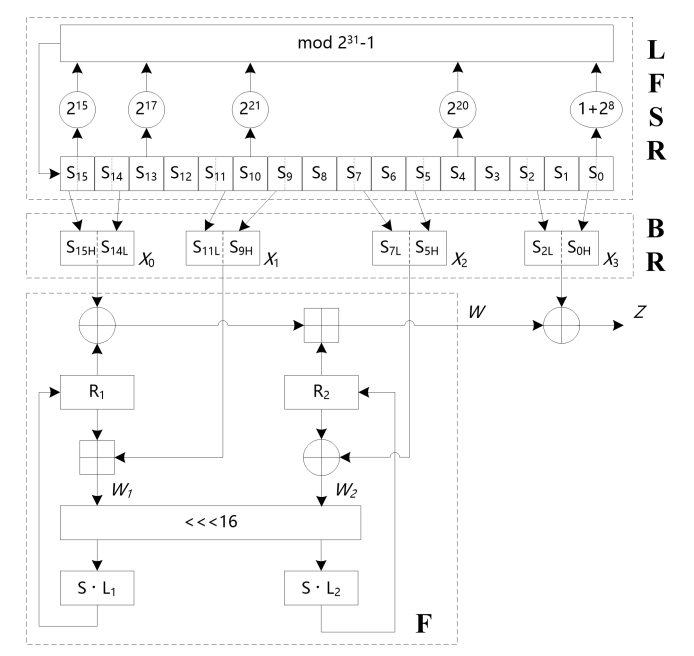
\includegraphics[height=.5\textheight]{../images/zuc_algo.png}
    \caption{ZUC 算法的流程图 \cite{zuc_standard}}
    \label{fig:zuc_algo}
\end{figure}


\section{算法的软硬件实现}

硬件设计使用的软件是 ISE 14.3,使用的 FPGA 型号为:XC6SLX75-2CSG484。在完成硬件设计、仿真和综合后,在实际环境中运行 ZUC 算法,并采集功耗曲线,用于后续的分析

软件实现使用的语言为 Python 3.6,运行平台为 Windows 10。软件部分的作用是在功耗分析过程中计算中间值以及对应的假设功耗值,并进行相关系数攻击和更多的处理。软件代码开源在本人的 GitHub 仓库中:https://github.com/Hansimov/zuc-attack。

\newpage

硬件电路的输入和输出端口如图 \ref{fig:circuit_io} 所示。

\begin{figure}[htbp]
    \centering
    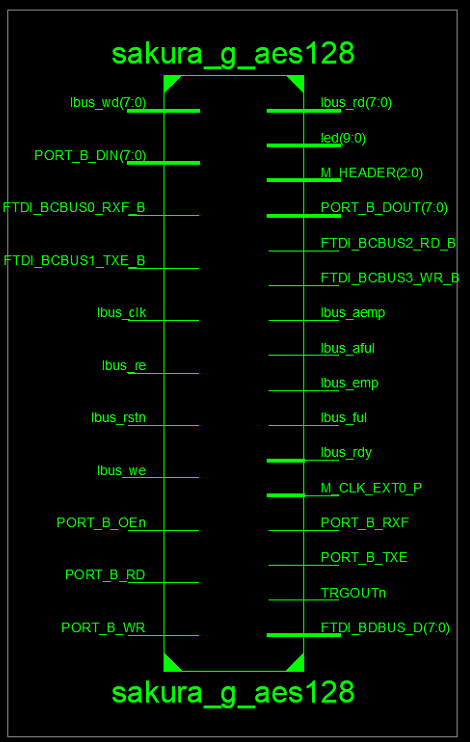
\includegraphics[height=.6\textheight]{../images/circuit_io.png}
    \caption{硬件电路的输入和输出端口}
    \label{fig:circuit_io}
\end{figure}

\newpage

硬件电路的内部结构如图 \ref{fig:circuit_more} 所示。

\begin{figure}[htbp]
    \centering
    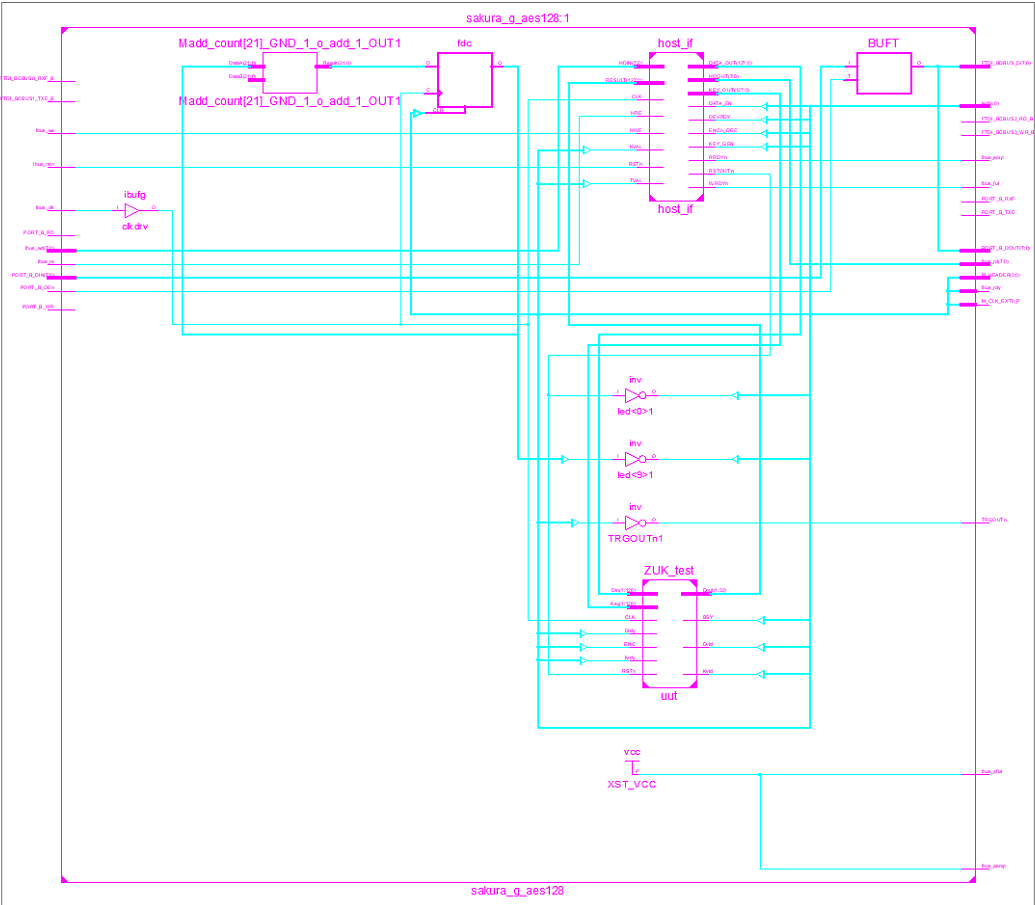
\includegraphics[height=.6\textheight]{../images/circuit_more.png}
    \caption{硬件电路的内部结构}
    \label{fig:circuit_more}
\end{figure}

\newpage


\section{本章小结}

本章首先讨论了 ZUC 算法的提出背景,介绍了其和通信行业发展的密切联系,并且指出了该算法对我国的重要意义。

然后我们讨论了 ZUC 算法的流程和结构,分别介绍了 ZUC 算法的三个部分,包括线性移位反馈寄存器、比特重组和非线性函数,并且讲解了初始化和工作的运行过程。

最后我们展示了 ZUC 算法的软硬件实现情况,给出了硬件电路的原理图,开源了软件代码,并且介绍了硬件部分和软件部分各自的用途。

我们讨论了功耗分析中简单功耗分析和差分功耗分析的异同,并且重点介绍了差分功耗攻击的基本流程和一般方法。

最后我们讨论了针对 ZUC 算法的差分功耗分析方案,除了介绍了传统的差分功耗分析的流程,还依据相关资料选取了有效的中间值,并且解释了这样选取的具体原因。

\chapter{对 ZUC 算法的功耗分析方案}
\label{chap:attack}

\section{差分功耗分析的一般步骤}
\label{sec:dpa}
功耗分析通常包含简单功耗分析(Simple Power Analysis)和差分功耗分析(Differential Power Analysis)。

简单功耗分析通常只需要少量的功耗曲线,就能揭示密码设备中的有用信息。简单功耗分析通常适用于功耗曲线特征较为明显的密码设备,比如出现明显的波峰和波谷,以及呈现出多个周期性的重复段落。如果攻击者对密码设备中运行的程序有一定的预备知识,那么就能推测出功耗曲线的不同段落在执行何种操作,就有可能进一步掌握设备的更多信息。

差分功耗分析则需要大量的功耗迹。大量功耗数据带来的好处就是更强大的分析和攻击能力,也不需要对设备的构造和执行的程序有详细的了解,一般情况下,只要掌握设备运行的算法流程就足够实施分析和攻击了。

因此,我们的关注重点就放在差分功耗分析上。

\vspace*{0.5\baselineskip}

下面我们来介绍一下差分功耗分析的一般流程:\cite{paa_cn}

\begin{enumerate}
\item \textbf{选取合适的算法中间值位置:}一个好的中间值,应该尽可能地区错误的猜测和正确的猜测。因此,在密码算法中,通常选择非线性函数的输出作为差分功耗分析的中间值。由于在运行算法和采集功耗时,攻击者往往只能获得明文或者密文,因此通常只能对算法的第一轮加密或者最后一轮加密进行攻击。因此,选取的中间值最好能够出现在第一轮或者的最后一轮。选取不同的中间值,会对攻击效果产生很大的影响,因此需要根据不同的算法和具体的实验条件,选取最合适的算法中间值。
\item \textbf{采集设备运行时的实际功耗曲线:}这一部分没有什么技术难度,不过值得一提的是,如果合理地选择功耗曲线采集和结束的位置,就能得到对齐较好的曲线,方便后续的分析和处理。采集环境也要尽可能地排除外界因素的干扰,以提高功耗曲线同数据和操作的相关性,增大信号的信噪比。更多具体的细节已经在上一小节阐述了。
\item \textbf{根据算法计算理论中间值:}对某个具体的密码算法而言,密钥通常是最重要也是最机密的信息,攻击者唯一无法知晓的也是这一部分。对全部位数的密钥进行穷举猜测是不可能做到的,因此攻击者常常需要在选择合适的中间值的前提下,尽可能地降低中间值和全部密钥之间的相关性。或者说,攻击者应该尽可能选取只依赖少部分密钥的中间值,这样就能大大减少猜测的可能情况,提高攻击的效率。由于密码算法通常是公开透明的,因此已知明文和猜测密钥的情况下,是可以计算出适合的理论中间值的。
\item \textbf{使用合适的功耗模型将理论中间值转换为假设功耗值:}算法的中间值通常是某个字节或者比特,和算法有关。由于中间值的值域很大,因此对所有可能的中间值建立一个具体的模型是不现实的。所以有必要采用合适的功耗模型,缩小猜测空间,将中间值转换成假设功耗值。常用的功耗模型包括汉明重量模型、汉明距离模型以及零值模型。功耗模型之间各有利弊,需要根据实际的实验情况和攻击效果选取最合适的模型。
\item \textbf{分析假设功耗值和实际功耗曲线,挖掘所需的信息:}这部分通常涉及到一定的统计学知识,需要攻击者具备较好的数学基础。在分析曲线的特征之前,通常还要对功耗曲线进行预处理,比如对齐和滤波,减少噪声,提高信噪比,从而能够更好地利用功耗曲线中的有效信息。此外,高效地处理大量的数据也是一个需要仔细考量的问题,差分功耗分析往往会采集成千上万甚至是百万条曲线,如何编写性能优异的算法,或者是并行化处理,都会很大程度上影响分析的速度和效果。除了常用的相关系数攻击之外,模板攻击也很有效。攻击者应该尽可能地设计好的算法,从而减少所需的功耗曲线条数,这样就能大大减少攻击的时间和成本。
\end{enumerate}

\vspace*{0.5\baselineskip}

图 \ref{fig:dpa} 展示了差分功耗分析攻击的第 3 -- 5 步。

\begin{figure}[htbp]

    \centering
    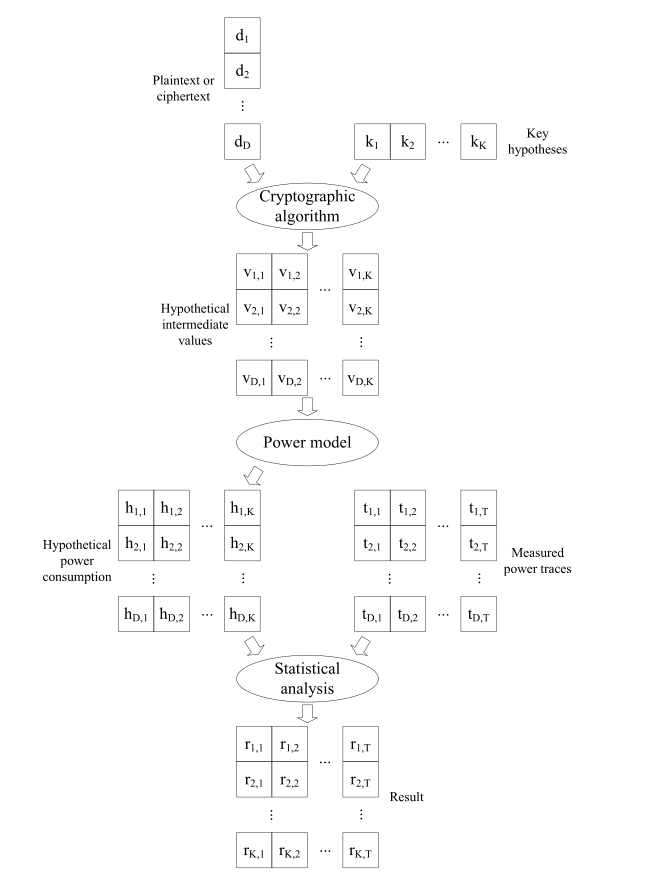
\includegraphics[height=.6\textheight]{../images/dpa.png}
    \caption{差分功耗分析的典型流程\cite{paa_en}}
    \label{fig:dpa}
\end{figure}

\section{寻找中间值}

在进行软件分析之前,我们首先要在硬件上实现 ZUC 算法电路,并采集其运行时的功耗。这部分相对简单,我们已经在 \ref{sec:hardware} 节中实现了硬件电路,而采集功耗的过程也很容易,因此这里不再赘述。

在 ZUC 算法中,唯一未知的信息就是初始的种子密钥,其他的常量和明文都是已知的。因此我们的攻击目的就是得到密钥的信息,也就是种子密钥的各个字节。

差分功耗攻击最核心的思想是,假设功耗值和实际功耗值之间是有关联的。而要想假设功耗值尽可能贴合实际功耗值,就需要选择合适的中间值。

一般而言,中间值通常选择算法中非线性变换的部分,因为如果输入稍有不同,非线性变换的输出就会出现较大的差异,从而正确的输入和错误的输入产生的差异将比线性变换更加明显,就可以有效地区分出正确的输入和错误的输入。

因此,我们第一步想到的是,把目光放在 ZUC 算法的非线性函数模块,看看能否从这个模块的附近找到合适的中间值。


\vspace*{0.5\baselineskip}

由于 ZUC 算法是分成三层的,第三层的非线性函数模块的输入,取决于第一层的线性反馈移位寄存器模块和第二层的比特重组模块的输出,而上面两层都对算法中的变量作了很多操作和运算,比如移位、剪切、粘贴、比特加、比特异或、素域模加,这就导致不同密钥字节彼此间的关联度很高。

密钥字节关联度很高的后果就是,我们很难对单个密钥字节进行猜测(只需要穷举 $2^8$ 种情况),这就导致我们必须穷举更多的情况(N 个密钥字节就对应 $2^{8 \times N}$ 种情况),一旦关联的密钥字节数较多,就几乎不可能对其穷举。

所以我们的首要任务,就是找到算法中尽可能独立的密钥字节。换句话说,如果在某个时刻,非线性函数模块的输出只和单个密钥字节相关,那么这个密钥字节就具有极强的独立性,我们也只需要穷举 $2^8$ 种情况就能攻出这个密钥字节。

我们需要对算法进行自顶向下地剖析,观察不同阶段哪些密钥字节参与了什么运算。

\vspace*{0.5\baselineskip}

我们从图 \ref{fig:zuc_algo} 中截取一部分,得到图 \ref{fig:zuc_lfsr_br},该图展示了线性反馈移位寄存器模块的输出、比特重组模块的全部以及非线性函数模块的输入。

\begin{figure}[htbp]
    \centering
    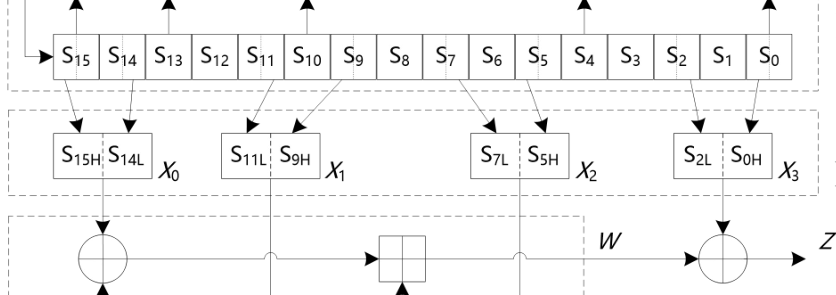
\includegraphics[width=0.8\textwidth]{../images/zuc_lfsr_br.png}
    \caption{线性反馈移位寄存器模块的输出、比特重组模块的全部以及非线性函数模块的输入}
    \label{fig:zuc_lfsr_br}
\end{figure}

\newpage

从图中可以看出,并不是任何时刻所有种子密钥字节都参与运算,以初始化阶段为例,{\cnsls zucInit} 的每一轮中,线性反馈移位寄存器的输出只和 8 个寄存器单元相关。线性反馈移位寄存器输出的便是比特重组的输入,见代码 \ref{lst:bitreorganization},我们这里将其再次写出来,方便参阅:

\begin{lstlisting}[style=myPython]
def bitReorganization():
    global x, s
    x[0] = s[15][0:16] + s[14][-16:]
    x[1] = s[11][-16:] + s[9][0:16]
    x[2] = s[7][-16:] + s[5][0:16]
    x[3] = s[2][-16:] + s[0][0:16]
\end{lstlisting}

那么这里的寄存器单元 {\cnsls s[i]} 又和什么有关呢?在变量初始化的代码 \ref{lst:varsinit} 中,我们可以找到如下语句:

\begin{lstlisting}[style=myPython]
...

def varsInit():
    ...
    for i in range(0, 16):
        s[i] = k[i] + d[i] + v[i]
    ...
\end{lstlisting}

也就是说,在 ZUC 算法中,线性反馈移位寄存器的每个 31 比特单元变量 {\cnsls s[i]} 是由种子密钥字节 {\cnsls k[i]}、给定的字符串常量单元 {\cnsls d[i]} 以及初始向量(输入的明文)字节 {\cnsls v[i]} 连接而成的。(可以参考表 \ref{table:symbol} 中各符号的说明。)

那么我们就可以对输入比特重组模块的 8 个字节进行拆解,找到和其相关的密钥字节:

\begin{lstlisting}[style=myPython]
    x[0] = s[15][0:16] + s[14][-16:]
         = (k[15][:] + d[15][0:8]) + (d[14][-8:] + v[14][:])

    x[1] = s[11][-16:] + s[9][0:16]
         = (d[11][-8:] + v[11][:]) + (k[9][:] + d[9][0:8])

    x[2] = s[7][-16:] + s[5][0:16]
         = (d[7][-8:] + v[7][:]) + (k[5][:] + d[5][0:8])

    x[3] = s[2][-16:] + s[0][0:16]
         = (d[2][-8:] + v[2][:]) + (k[0][:] + d[0][0:8])
\end{lstlisting}

这里提一句,在 Python 中,{\cnsls s[15][0:16]} 表示 {\cnsls s[15]} 的前 16 比特,也就是第 0 到 15 比特,而不是第 0 到 16 比特,相当于索引的区间是左闭右开。{\cnsls s[14][-16:]} 则表示 {\cnsls s[14]} 的末 16 比特,{\cnsls k[15][:]} 表示 {\cnsls k[15]} 的全部比特(8 位)。

从拆解结果可以看到,相关的密钥字节有且仅有:{\cnsls k[15], k[9], k[5], k[0]}。

那么,在非线性函数模块中,是不是这 4 个又都参与运算了呢?并不是。

\vspace*{0.5\baselineskip}

\newpage

我们再截取图 \ref{fig:zuc_algo} 的另外一部分,得到图 \ref{fig:zuc_br_f},稍作观察。

\begin{figure}[htbp]
    \centering
    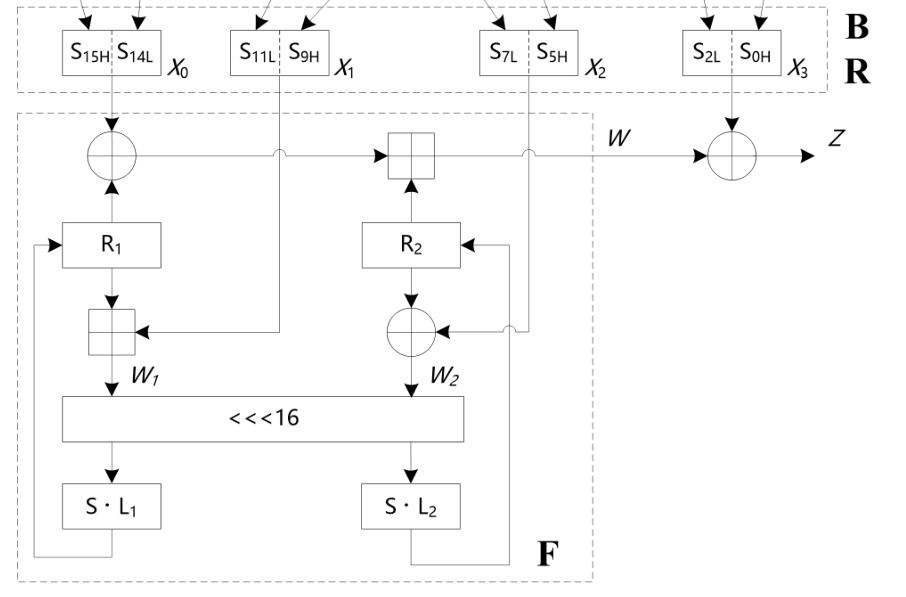
\includegraphics[width=0.8\textwidth]{../images/zuc_br_f.png}
    \caption{比特重组模块和非线性函数模块}
    \label{fig:zuc_br_f}
\end{figure}

从图中的数据流向可以看出,{\cnsls x[0]} 和 {\cnsls x[3]} 并没有参与非线性函数模块的内部操作,而只是和记忆单元 {\cnsls r1} 和 {\cnsls r2} 作了简单的运算,用于输出密钥流。

因此,真正参与非线性函数模块的内部操作的,只有 {\cnsls x[1]} 和 {\cnsls x[2]},与之相关的密钥字节便是 {\cnsls k[9]} 和 {\cnsls k[5]}。

下面我们再来看一下 {\cnsls k[9]} 和 {\cnsls k[5]} 又是如何参与非线性函数中的运算的。

这里我们将非线性函数模块的代码 \ref{lst:nonlinearfunction} 重写一遍,方便查看:

\begin{lstlisting}[style=myPython]
def nonLinearFunction():
    global w, x, r1, r2
    w = binaryAdd(binaryXor(x[0], r1), r2)
    w1 = binaryAdd(r1, x[1]) `\label{line:w1}`
    w2 = binaryXor(r2, x[2]) `\label{line:w2}`
    r1 = sboxOfZuc(linearTransform(w1[-16:]+w2[0:16], 1)) `\label{line:r1}`
    r2 = sboxOfZuc(linearTransform(w2[-16:]+w1[0:16], 2)) `\label{line:r2}`
\end{lstlisting}

从第 \ref{line:r1} -- \ref{line:r2} 行可以看出,{\cnsls r1} 和 {\cnsls r2} 的值与 {\cnsls w1} 和 {\cnsls w2} 均相关,而 {\cnsls w1} 与 {\cnsls x[1]} 相关,{\cnsls w2} 与 {\cnsls x[2]} 相关。

\newpage

让我们将几个变量做一下拆解,以便更好地理清它们之间的关系:

(我们用\ {\color{blue} $a \Leftarrow b$} 表示\ {\color{blue} $a$ 取决于 $b$})

\begin{lstlisting}[style=myPython]
r1 `$\Leftarrow$` w1[-16:] + w2[0:16] 
   `$\Leftarrow$` x[1][-16:] + x[2][0:16]
   `$\Leftarrow$` (k[9][:] + d[9][0:8]) + (d[7][-8:] + v[7][:])

r2 `$\Leftarrow$` w2[-16:] + w1[0:16]
   `$\Leftarrow$` x[2][-16:] + x[1][0:16]
   `$\Leftarrow$` (k[5][:] + d[5][0:8]) + (d[11][-8:] + v[11][:])
\end{lstlisting}

我们惊喜地发现:\textbf{{\cnsls r1} 仅和密钥字节 {\cnsls k[9]} 相关,而 {\cnsls r2} 仅和密钥字节 {\cnsls k[5]} 相关!}

图 \ref{fig:zuc_attack} 展示了这一重要的关系。

\begin{figure}[htbp]
    \centering
    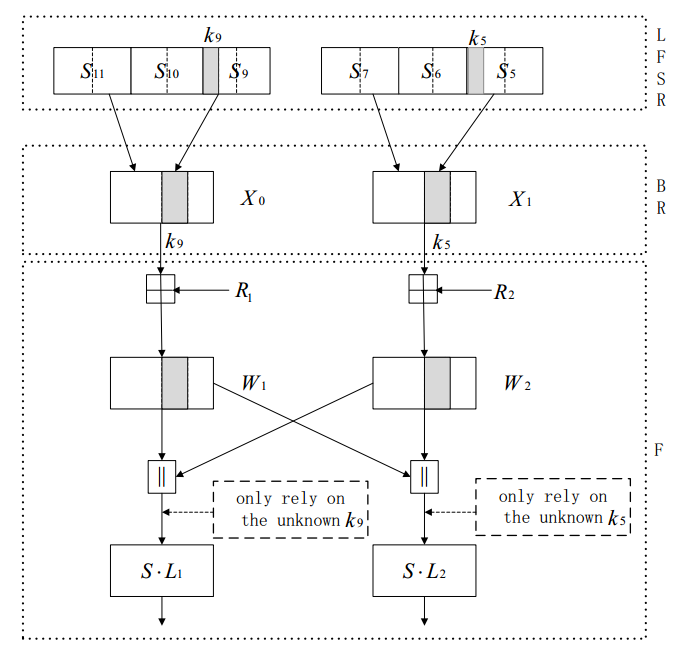
\includegraphics[height=.5\textheight]{../images/zuc_attack.png}
    \caption{在 {\cnsls zucInit} 第 1 轮中,{\cnsls r1} 仅和密钥字节 {\cnsls k[9]} 相关,而 {\cnsls r2} 仅和密钥字节 {\cnsls k[5]} 相关 \cite{zuc_attack_tangming}}
    \label{fig:zuc_attack}
\end{figure}

也就是说,如果将 {\cnsls r1} 或者 {\cnsls r2} 的输出作为中间值的话,我们就只需要猜测单个字节,也就是 $2^8$ 种情况,所花的代价非常小,可行性也非常高。

\newpage

\section{构建密钥推算链条}

然而,我们在上一节中的方案遗漏了两个细节。

第一个遗漏的细节是,在非线性函数模块的代码的第 \ref{line:w1} -- \ref{line:w2} 行中,{\cnsls w1} 不仅取决于 {\cnsls x[1]},还取决于{\cnsls r1},同样地,{\cnsls w2} 不仅取决于 {\cnsls x[2]},还取决于{\cnsls r2}。而 {\cnsls r1} 和 {\cnsls r2} 又是和上一轮非线性函数的结果相关的。

这里就出现了一个问题:如果 {\cnsls r1} 和 {\cnsls r2} 和上一轮非线性函数的结果相关,而要想知道上一轮非线性函数的结果,又需要知道上一轮中相关密钥字节,可是密钥字节正是我们未知的信息。似乎陷入了一个死循环。

经过思索,我们终于找到了问题的突破口:在第 1 轮算法初始化阶段 {\cnsls zucInit} 的非线性函数模块 {\cnsls nonLinearFunction} 中,{\cnsls r1} 和 {\cnsls r2} 的初始值是全 0。

可以参考变量初始化的代码 \ref{lst:varsinit} 的这一段:

\begin{lstlisting}[style=myPython]
...

def varsInit():
    ...
    r1 = [0] * 32
    r2 = [0] * 32
\end{lstlisting}

这样,我们就可以将全 0 作为 {\cnsls r1} 和 {\cnsls r2} 的初始值,代入到第 1 轮 {\cnsls zucInit} 的 {\cnsls nonLinearFunction} 中计算中间值。

换句话说,在 {\cnsls zucInit} 的第 1 轮中,除了密钥字节,其他的变量值都是已知的。这样,我们就可以计算出中间值,进行功耗分析,攻击出对应密钥字节,再将攻出来的字节代入到算法中,得到下一轮的相关值,这样就可以攻击出后续的密钥字节。

\vspace*{0.5\baselineskip}

然而事实并没有我们想象的这么简单,事实上,以 {\cnsls r1} 和 {\cnsls r2} 作为中间值,只能攻击 {\cnsls zucInit} 的前 5 轮。也就是说,通过这种方法可以攻击出来的密钥字节为:{\cnsls k[9], k[5]; k[10], k[6]; k[11], k[7]; k[12], k[8]; k[13](, k[9])}。(第 5 轮中攻出的 {\cnsls k[9]} 已经在第 1 轮攻出。)

为什么只能攻击前 5 轮呢?又为什么是这几个密钥字节呢?

\vspace*{0.5\baselineskip}

这也就引出了第二个遗漏的细节:在 {\cnsls zucInit} 的每一轮中,线性反馈移位寄存器的每个寄存器单元都会向右平移一个单元。参见代码 \ref{lst:lfsr} 中的这一段:

\begin{lstlisting}[style=myPython]
def lfsrInit():
    ...
    for i in range(0,16):
    s[i] = s[i+1]

def lfsrWork():
    ...
    for i in range(0,16):
    s[i] = s[i+1]
\end{lstlisting}

\newpage

那么,我们之前所谈论的 {\cnsls k[9]} 和 {\cnsls k[5]} 只是线性反馈移位寄存器中对应位置(第 9 个记忆单元和第 5 个记忆单元)的密钥字节,而不是原始的 {\cnsls k[9]} 和 {\cnsls k[5]},只有在 {\cnsls zucInit} 的第 1 轮 {\cnsls nonLinearFunction} 中,才是真正的 {\cnsls k[9]} 和 {\cnsls k[5]}。

事实上,在 {\cnsls zucInit} 的第 N 轮 {\cnsls nonLinearFunction} 中,和 {\cnsls r1} 相关的应当是原始密钥字节中的 {\cnsls k[8+N]},和  {\cnsls r2} 相关的应当是原始密钥字节中的 {\cnsls k[4+N]}。这也就是我们之前所列的,前 5 轮中可以攻出来的密钥字节的递推公式。

这里我们就碰到了关键的问题,到第 6 轮时,第 1 轮中的 {\cnsls s[16]$_1$} 已经移动到了这里的 {\cnsls s[11]$_6$} 处。(为了便于之后区分初始化阶段不同轮中线性反馈移位寄存器的单元变量,我们用 {\color{blue} {\cnsls s[i]$_n$}} 表示 {\color{blue} 第 {\cnsls n} 轮中线性反馈移位寄存器第 {\cnsls i} 个记忆单元变量的值},事实上,{\cnsls s[16]$_j$} = {\cnsls s[11]$_{j+5}$}。)

此时,如果想得到 {\cnsls r1} 的值,就必须知道 {\cnsls x[1]} 的值,而 {\cnsls x[1]} 的值是取决于 {\cnsls s[11]$_1$} 的,见代码 \ref{lst:bitreorganization} 的这一段:

\begin{lstlisting}[style=myPython]
def bitReorganization():
    ...
    x[1] = s[11][-16:] + s[9][0:16]
    ...
\end{lstlisting}

\vspace*{0.5\baselineskip}

问题的根源就在于此:第 6 轮中的 {\cnsls s[11]$_6$} 对应的是第 1 轮的 {\cnsls s[16]$_1$},而 {\cnsls s[16]$_1$} 的计算过程牵扯到几个其他密钥字节,参见代码 \ref{lst:lfsr} 的这一段:

\begin{lstlisting}[style=myPython]
def lfsrInit():
    global k_hex, k, v_hex, v, d, s, w
    shift_bits_list  = [15, 17, 21, 20, 8, 0] `\label{line:shiftbits}`
    shift_index_list = [15, 13, 10, 4, 0, 0] `\label{line:shiftindex}`
    xv = [0] * 31
    for i in range(0, len(shift_bits_list)):
        s_i_shifted = circShiftLeft(s[shift_index_list[i]], shift_bits_list[i])
        xv = modAdd_2e31m1(xv, s_i_shifted)
    s[16] = modAdd_2e31m1(shiftLeft(w, -1), xv)
    if s[16] == [0]*31:
        s[16] = [1]*31
    ...
\end{lstlisting}

因此,从 {\cnsls zucInit} 的第 6 轮开始,就不能再简单地用 {\cnsls r1} 和 {\cnsls r2} 作为中间值了。因为相关的密钥字节不再只有单个,而是多个,所需要猜测的可能大大增加。

事实上,在 {\cnsls zucInit} 的第 6 轮中,需要同时穷举 4 个密钥字节: {\cnsls k[15], k[14], k[4], k[0]}。也就是说,需要猜测 $2^{32}$ 种情况。

\newpage

我们解释一下为什么第 6 轮需要同时穷举这 4 个密钥字节。我们在上文指出,{\cnsls zucInit} 第 6 轮中要用到的 {\cnsls s[11]$_6$} 对应的第 1 轮中的 {\cnsls s[16]$_1$},而第 1 轮中的 {\cnsls s[16]$_2$} 和 {\cnsls k[15], k[13], k[10], k[4], k[0]} 相关。可以参考上面线性反馈移位寄存器初始化模式代码的第 \ref{line:shiftindex} 行:

\begin{lstlisting}[style=myPython]
def lfsrInit():
    ...
    shift_bits_list  = [15, 17, 21, 20, 8, 0]
    shift_index_list = [15, 13, 10, 4, 0, 0]
    ...
\end{lstlisting}

{\cnsls shift\_index\_list} 列出了需要移位的字节,{\cnsls shift\_bits\_list} 列出了对应位置的字节需要移多少位,并且相关的字节在移位后还要参与后续的素域模 $2^{31}-1$ 加运算,因此无法单独攻出各个密钥字节,必须同时穷举所有的未知字节。

在第 1 轮中,这里的移位的 {\cnsls s[i]$_1$} 和 {\cnsls k[i]} 相关。事实上,在第 N 轮中,发生移位的 {\cnsls s[i]$_N$} 和 {\cnsls k[i+N-1]} 相关。

因此,从 {\cnsls shift\_index\_list} 就能够得知和第 1 轮中 {\cnsls s[16]$_1$} 相关的密钥字节是:{\cnsls k[15], k[13], k[10], k[4], k[0]}。不过由于 {\cnsls k[10]} 可以在第 2 轮中攻出,{\cnsls k[13]} 可以在第 5 轮中攻出,因此实际上未知的只有 {\cnsls k[15], k[4], k[0]}。

又由于第 6 轮中,和 {\cnsls r1} 相关的密钥字节是 {\cnsls k[14]}(未知),和 {\cnsls r2} 相关的密钥字节是 {\cnsls k[10]}(已攻出),故需要猜测的密钥字节还要再加上 {\cnsls k[14]}。

因此,第 6 轮中需要同时对 {\cnsls k[15], k[14], k[4], k[0]} 这 4 个密钥字节进行穷举,共计 $2^{32}$ 种情况。

\vspace*{0.5\baselineskip}

此时,截至第 6 轮结束,我们可以攻出的字节有:{\cnsls k[9], k[5]; k[10], k[6]; k[11], k[7]; k[12], k[8]; k[13]; k[15], k[14], k[4], k[0]}。剩下的未知的密钥字节只有:{\cnsls k[1], k[2], k[3]}。

\vspace*{0.5\baselineskip}

类似第 6 轮中的思路,在第 7 轮中的 {\cnsls s[11]$_7$} 对应第 2 轮输出的 {\cnsls s[16]$_2$}。我们在上文提过,在第 N 轮中,发生移位的 {\cnsls s[i]$_N$} 和 {\cnsls k[i+N-1]} 相关,因此 {\cnsls s[16]$_2$} 又依据 {\cnsls shift\_index\_list},可以得知和 {\cnsls s[16]$_2$} 相关的密钥字节为 {\cnsls k[14], k[11], k[5], k[1]},这里仅有 {\cnsls k[1]} 未知。又第 7 轮中的 {\cnsls r1} 和密钥字节 {\cnsls k[11]} 相关,{\cnsls r2} 和密钥字节 {\cnsls k[15]} 相关,而 {\cnsls k[11]} 和 {\cnsls k[11]} 都是已知的。因此只需要猜测 {\cnsls k[1]},也就是穷举 $2^8$ 种情况。

仿照上面的流程,我们可以在第 8 轮中攻出 {\cnsls k[2]},在第 9 轮中攻出 {\cnsls k[3]}。

\vspace*{0.5\baselineskip}

至此,我们就将所有的密钥字节攻击出来了,所需要猜测的情况总数为:$2^8 \times (9+3) + 2^{32}$。

\newpage

\section{计算假设功耗值}

选好了中间值的位置,我们就可以计算出所有密钥猜测(从 0 到 255,也即 16 进制的 00 到 FF)对应的中间值。

然后我们要选择合适的功耗模型,通过中间值计算出理论功耗值(或者称作假设功耗值)。这一步骤的目的是将中间值映射到一个更小的空间,便于区分不同特征的曲线。

我们这里选择汉明重量作为功耗模型。一个仅由 0 和 1 构成的向量的汉明重量,等于该向量中 1 的个数。

因此,给定一个中间值向量,就能得到一个对应的汉明重量,也就是其假设功耗值。

汉明重量模型有效的前提假设是:设备产生的功耗,与其操作的数据中 1 的个数是相关的。

选择汉明重量模型的原因是,计算相对简单,而且其有效性假设在现实中一般都能成立。

\section{计算相对相关系数}

在采集到实际功耗曲线,并通过中间值算出假设功耗值后,我们就可以计算假设功耗值矩阵和实际功耗值矩阵之间的相关系数了。

相关系数表征了假设功耗值和实际功耗值之间的关联程度,相关系数越高,二者之间的关联度就越高。

计算相关系数的公式如下:

\begin{equation*}
r = \frac{\sum\limits_{i=1}^{n}(X_i-\overline{X})(Y_i-\overline{Y})}{\sqrt{\sum\limits_{i=1}^n(X_i-\overline{X})^2}\sqrt{\sum\limits_{i=1}^n(Y_i-\overline{Y})^2}}
\end{equation*}

其中,$r$ 表示样本相关系数,$X_i$ 表示假设功耗值的样本点,$Y_i$ 表示实际功耗值的样本点,$n$ 表示样本点数。

\vspace*{0.5\baselineskip}

我们对相关系数矩阵稍作处理,得到“相对相关系数”,目的是为了更好地挖掘有效信息。处理过程如下:

先对相关系数矩阵取绝对值,这是因为不论相关系数是正是负,只要绝对值够大,就表明有显著的相关性。再取每一行中最大的前 5 个值,计算平均值,即可得到“相对相关系数”。这是因为实际功耗曲线上只有极少数的时间点有功耗信息的泄露,我们只需要泄露最明显的那一些点,如果让很多不相关的时刻上的相关系数也参与运算,就会降低信噪比,掩盖掉有用的信息。

\vspace*{0.5\baselineskip}

最后我们比较不同密钥猜测的相对相关系数,值最大的即对应最优的密钥猜测。

\section{实现完整的差分功耗分析}

我们在前面详细讲解了攻击的方案,这里我们为了突出功耗分析的重要思想,选取了一个易于理解的典型,仅以 {\cnsls zucInit} 第 1 轮中 {\cnsls r2} 的输出作为中间值,来攻击 {\cnsls k[5]}。

将上面的方案串联起来,就能得到完整的功耗分析流程,代码 \ref{lst:whole_attack} 是这一流程的软件实现。

\newpage

\begin{lstlisting}[style=myPython,label={lst:whole_attack},caption={差分功耗分析攻击的完整流程}]
# Read traces
    sample_mat = [[]]*trace_num
    for i in range(0, trace_num):
        sample_mat[i] = getTraceSample(trs_file, header_end, i, sample_num, offset)
    hw_mat = [[0]*trace_num for _ in range(256)]

# Calculate inter values and hammingweight
    for i in range(0, trace_num):
        for k in range(0, 256):
            inter_val = calcInterValue(i, k)
            hw_mat[k][i] = calcHammingWeight(inter_val)

# Calculate relative correlation matrix of guessing key
    sample_mat = np.array(sample_mat)
    hw_mat = np.array(hw_mat)
    for n in [100, 200, 500, 1000, 2000, 5000, 10000, 20000]:
        corr_maxn = [[0]*5 for _ in range(256)]
        for k in range(0,256):
            for j in range(0, sample_num):
                corr_mat[k][j] = abs(np.corrcoef(hw_mat[k][0:n], sample_mat[0:n, j])[0][1])
            corr_maxn[k] = heapq.nlargest(len(corr_maxn[0]), corr_mat[k])
              corr_avg[k] = np.mean(corr_maxn[k])
  
          corr_max = max(corr_avg)
          key_max = corr_avg.index(corr_max)
\end{lstlisting}

由于篇幅限制,这里略去了很多细节,只展示了算法中最核心的部分。

我们将在下一章给出实验的具体结果以及详细分析。


\section{本章小结}


本章首先讨论了功耗分析中简单功耗分析和差分功耗分析的异同,并且重点介绍了差分功耗攻击的基本流程和一般方法。

其次我们试图寻找合适的中间值,对算法进行了深入的挖掘,并且发现了合适的中间值。

然后我们对算法进行了进一步的剖析,探讨了遗漏的细节,并且补全了对剩余密钥字节的攻击方案。

接着我们选取了合适的功耗模型,并进行相关系数攻击。

最后我们以一个典型的密钥字节作为攻击对象,展示了将功耗分析技术完整地用于现实场景的过程。

%# -*- coding: utf-8-unix -*-
%%==================================================
%% 04_results.tex % 4k
%%==================================================


\chapter{实验结果与分析}

\label{chap:results}

\section{功耗曲线}

按照在 \ref{sec:collect} 节所述的流程,在密码算法电路运行时,采集其功耗,并记录存储到计算机上。本次实验一共采集了 100 万条功耗曲线,实际用到的为前 2 万条。密码算法跑在普通的 FPGA 上,这里的功耗值对应的具体物理量,实际上是电路电源线上的总电流。 \cite{zuc_fpga} \cite{zuc_fpga_en}

由于我们的攻击针对的是 ZUC 算法的初始化阶段,因此只储存了初始化阶段的功耗点。初始化阶段一共有 32 轮,这里只记录了前 27 轮,不过这也已经足够我们使用了。

\vspace*{\baselineskip}

图 \ref{fig:traces} 展示了第 1、20、200、2000 和 20000 条功耗曲线的波形。

从图中可以得到这样一些信息:

\begin{enumerate}
    \item \textbf{时钟频率以及电路运行状况稳定。}\\
    图中的曲线在各个时间点处的峰值基本对齐,说明时钟频率非常稳定,并且每次运行算法所花费的时间几乎是相同的。从抽取的曲线来看,波形也几乎一致。这意味着我们可以免去对齐曲线这部分预处理的工作,降低了工作量,清晰的轮廓也从侧面反映了采集得到的功耗曲线质量较高。因此得到这样的曲线是非常令人满意的。
    \item \textbf{采集到的曲线包含了密钥装载阶段和前 27 轮初始化。}\\
    前面一段持续的高功耗,应该是算法电路的启动,以及相关数据载入内存并交由控制器的部分,其中的一个尖峰,可能是密钥装载的阶段。之后可以看到 27 个特征相似的波形,毫无疑问,这是算法中初始化阶段的 27 轮循环操作。图中的尖峰特征还是非常明显的,然而这并不代表一定会有密钥信息的泄露。诚然,在很多情况下,功耗的尖峰和明显的起伏,很可能是泄露点,但是具体的泄露位置以及泄露程度,还是需要后续的分析才能确定。
\end{enumerate}

\begin{figure}[htbp]
    \centering

    \begin{subfigure}{1.0\textwidth}
        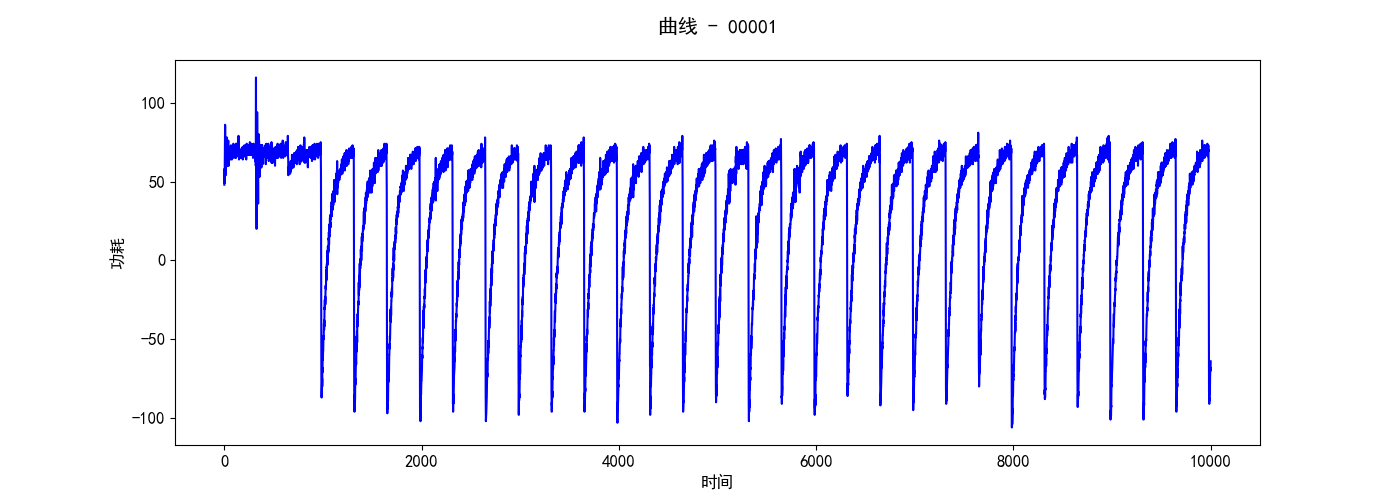
\includegraphics[height=.17\textheight, width=1.0\textwidth]{../images/trace_00001.png}
        % \caption{第 00001 条功耗曲线}
    \end{subfigure}
    \begin{subfigure}{1.0\textwidth}
        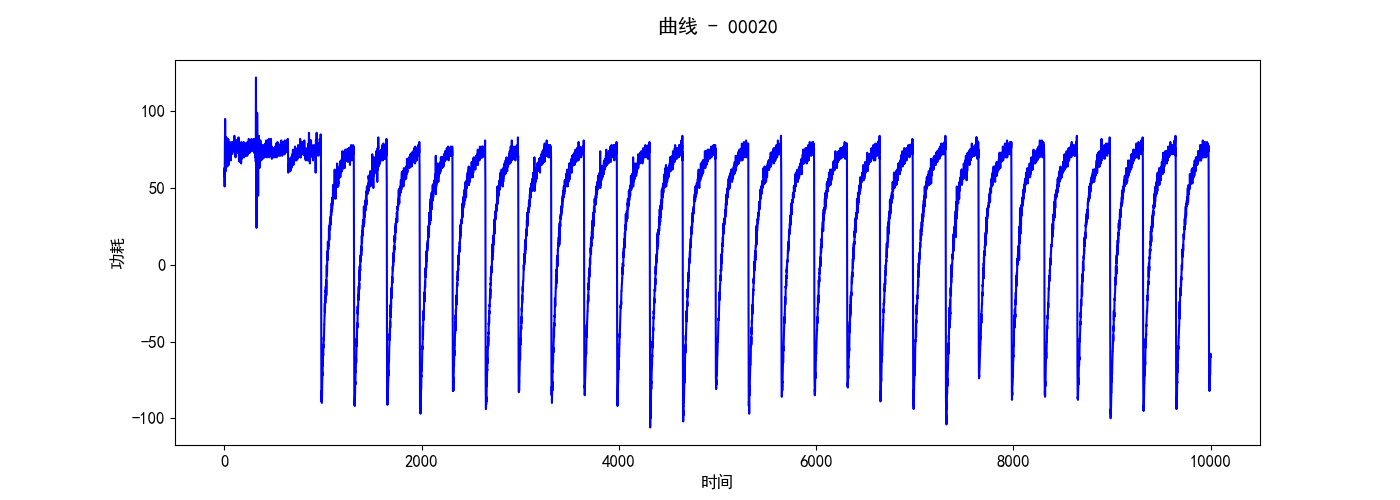
\includegraphics[height=.17\textheight, width=1.0\textwidth]{../images/trace_00020.png}
        % \caption{第 00020 条功耗曲线}
    \end{subfigure}
    \begin{subfigure}{1.0\textwidth}
        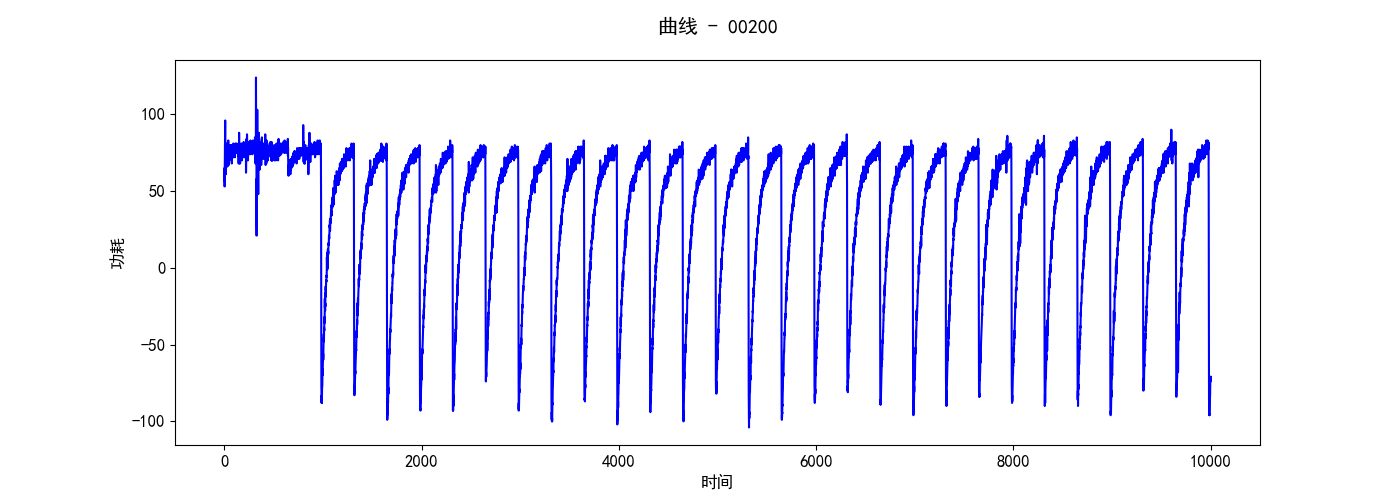
\includegraphics[height=.17\textheight, width=1.0\textwidth]{../images/trace_00200.png}
        % \caption{第 00200 条功耗曲线}
    \end{subfigure}
    \begin{subfigure}{1.0\textwidth}
        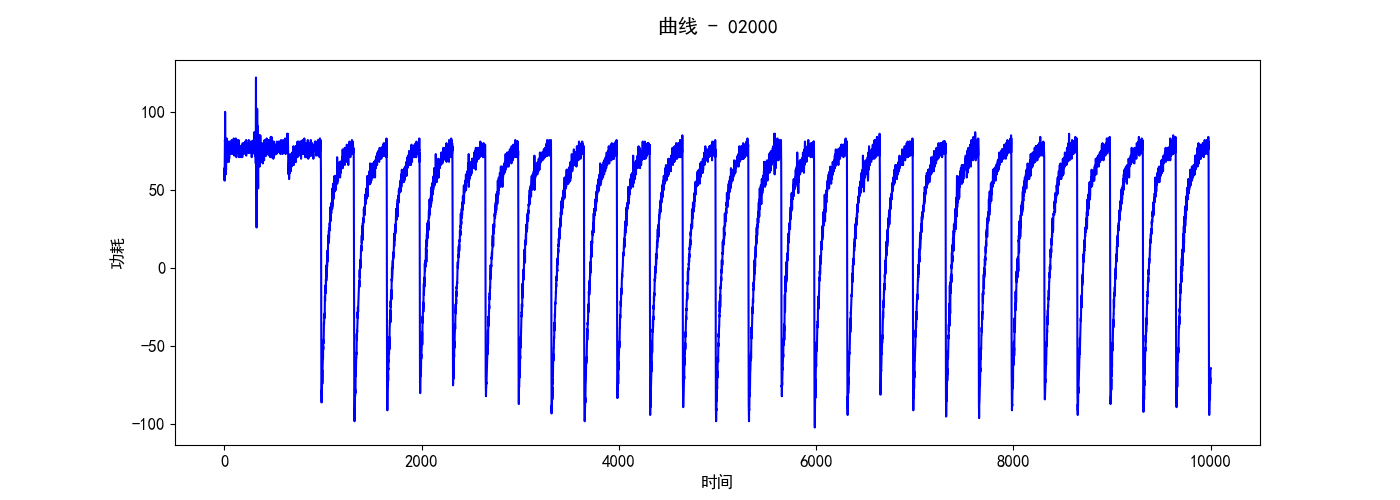
\includegraphics[height=.17\textheight, width=1.0\textwidth]{../images/trace_02000.png}
        % \caption{第 02000 条功耗曲线}
    \end{subfigure}
    \begin{subfigure}{1.0\textwidth}
        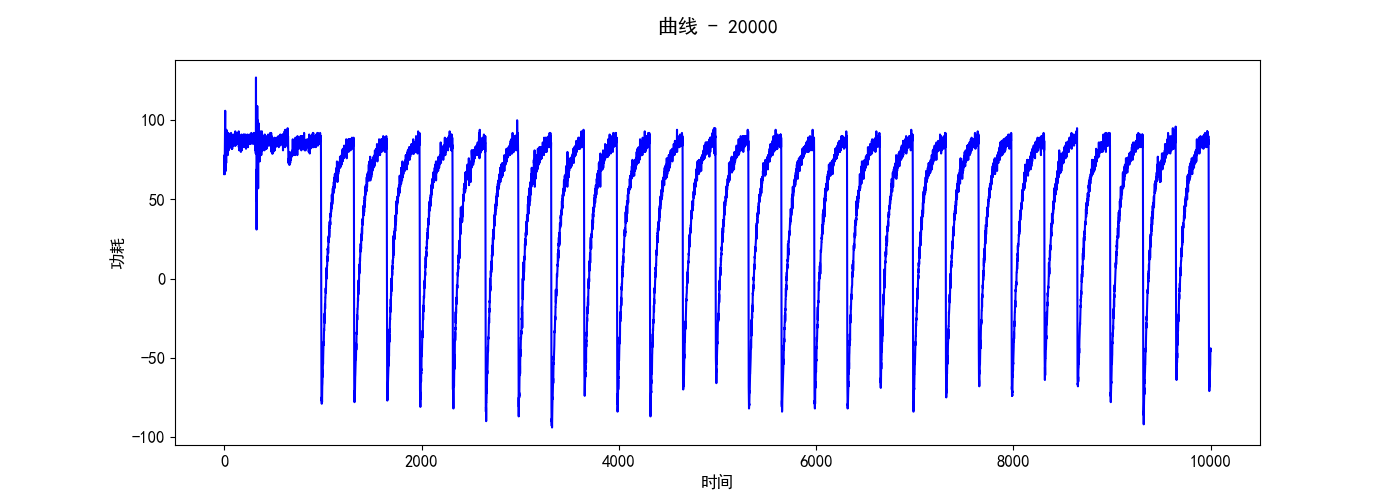
\includegraphics[height=.17\textheight, width=1.0\textwidth]{../images/trace_20000.png}
        % \caption{第 20000 条功耗曲线}
    \end{subfigure}

    \caption{ZUC 算法初始化阶段硬件电路的功耗曲线}

    \label{fig:traces}

\end{figure}

\newpage

\section{不同密钥猜测的相对相关系数}

按照在上一章中分析的流程,猜测不同的 k5 对应的中间值,总共有 256 种可能的情况。然后利用汉明重量模型,将其转换成假设功耗值,求解与实际功耗值之间的相关系数。由于选取的中间值在初始化阶段第一轮末尾,因此我们将攻击的部位选取为覆盖第一轮和第二轮的功耗点,因此实际参与计算的功耗点数在 500 左右。

我们将这些点上的相关系数求绝对值后,取最大的前 5 个值求平均,得到可以参考的平均相关系数。这样处理的目的是为了减小误差,防止某些无效的相关系数值遮盖了有效的值。为了和真正的“相关系数”作区分,我这里将其称为“相对相关系数”。

\vspace*{\baselineskip}

图 \ref{fig:keyguess} 展示了使用不同功耗曲线条数进行攻击,得到的 256 个密钥猜测的相对相关系数。横轴是密钥字节猜测的 10 进制值,纵轴是相对相关系数,绿色的虚线代表相对相关系数最高的猜测字节。

从图中可以得到这样一些信息:

\begin{enumerate}
    \item \textbf{当攻击的功耗曲线数目达到一定值之后,字节 171(AB)的相对相关系数保持最高。}\\
    因此 k5 最有可能是 171(AB)。而实验预设的密钥是“01 23 45 67 89 AB CD EF 01 23 45 67 89 AB CD EF”(k0 到 k15),k5 恰好是“AB”,这也就表明我们的最佳猜测是正确的,攻击成功。
    \item \textbf{在使用的功耗曲线条数为 100 时,根据相对相关系数猜测的最佳密钥字节是 43(2B),而这个猜测结果是错误的。}\\
    这表明当攻击使用的功耗曲线数目较少时,得到的结果可信度较低,这时最佳密钥字节猜测还不够稳定。因此在攻击时一定要测试猜测结果的稳定性,选用的方法就是使用更多的功耗曲线。\\
    一个值得注意的细节是,尽管猜测错误,但是“2B”对应的二进制值是“00101011”,和正确的“AB”对应的二进制值“10101011”仅仅相差一个比特。虽然不同字节在非线性变换后,输出的差异一般非常大,因此错误猜测和正确结果之间的关联一般没有参考价值,但是这里的细节可能表明,密码算法的非线性变换部分或许有微小的瑕疵,从而造成了某些不同的字节在输出后差异并没有想象中的那么大,攻击者有可能通过选择合适的明文,来扩大非线性变换中的漏洞,更高效地破解相关密钥字节。不过尚缺乏充分的实验来证明这一猜想。
    \item \textbf{当使用的功耗曲线条数越来越多时,正确的密钥字节对应的相对相关系数明显高于错误的密钥字节。}\\
    这个现象的原因是显然的,随着功耗曲线条数的增多,错误密钥字节产生的中间值与正确密钥字节产生的中间值差异愈发明显,偶然性渐渐被必然性覆盖。因此,选用尽可能多的功耗曲线条数,一般可以提高攻击的成功率。
    \item \textbf{随着功耗曲线条数的增多,相对相关系数的最大值呈减小趋势。}\\
    比如使用的功耗曲线条数为 1000 时,最高相对相关系数约为 0.25,而当使用的功耗曲线条数到 20000 时,最高相对相关系数已经降低到大概 0.15 了。事实上,不仅最高相对相关系数在减小,所有密钥字节猜测对应的相对相关系数,整体上都在减小。这是因为,尽管假设功耗值(依据理论中间值和功耗模型计算得到)和实际功耗值之间存在一定的联系,但这种联系不一定是强正相关的。所以当攻击采用的功耗曲线条数很多时,假设功耗值与实际功耗值之间不相关的部分占比就会变大。\\
    为什么假设功耗值与理论功耗值有不相关的地方呢?直观的原因是,电路执行某个操作的时间并不是每一次都完全对齐的,或者某些频率的噪声对曲线的波形产生了影响。还有一些更底层更根本的原因,比如选取的功耗模型并不能真正反映实际的功耗值大小,我们此次采用的汉明重量模型,是基于“设备的功耗和操作的数据中的 1 的个数有关”这一假设,而事实可能并非如此:设备的功耗可能不仅仅和数据中 1 的个数有关,既可能和数据中 0 的个数有关,也可能和从 0 到 1 或者从 1 到 0 的比特数目有关,而且设备的功耗也不完全取决于操作的数据,还可能和控制命令也有关系,或者操作相关数据的同时,还可能在运行其他的指令、操作其他不相关的数据。\\
    既然这样,那么为什么本次实验中,功耗曲线条数越多,正确密钥猜测的相对相关系数越突出呢?这是因为,正确密钥字节对应的假设功耗值和实际功耗值中相关的部分比例高于不相关部分的比例。功耗曲线数目的增加并不会改变这种比例,因此尽管整体上相关系数的绝对数值降低了,但是正确的密钥字节对应的假设功耗值仍旧比错误的密钥字节更接近于实际功耗值。\\
    因此,尽管随着功耗曲线条数的增加,整体的相对相关系数的数值存在减小趋势,但是这也降低了偶然因素的影响,使得正确密钥字节对应的假设功耗值与实际功耗值之间的关联度,更加稳定地优于错误的密钥猜测。


\end{enumerate}

\begin{figure}[htbp]
    \centering

    \begin{subfigure}{1.0\textwidth}
        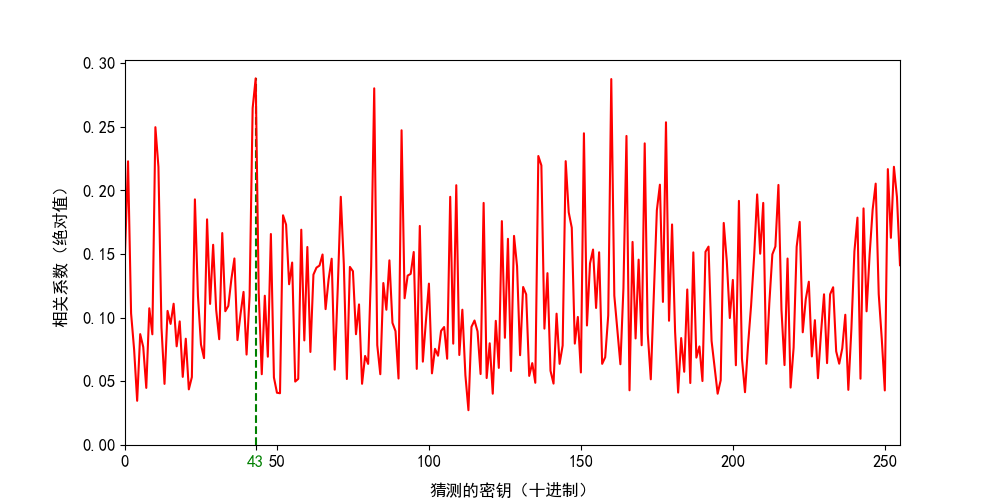
\includegraphics[height=.21\textheight, width=1.0\textwidth]{../images/keyguess_100.png}
        \caption{攻击使用的功耗曲线条数:100}
    \end{subfigure}
    \begin{subfigure}{1.0\textwidth}
        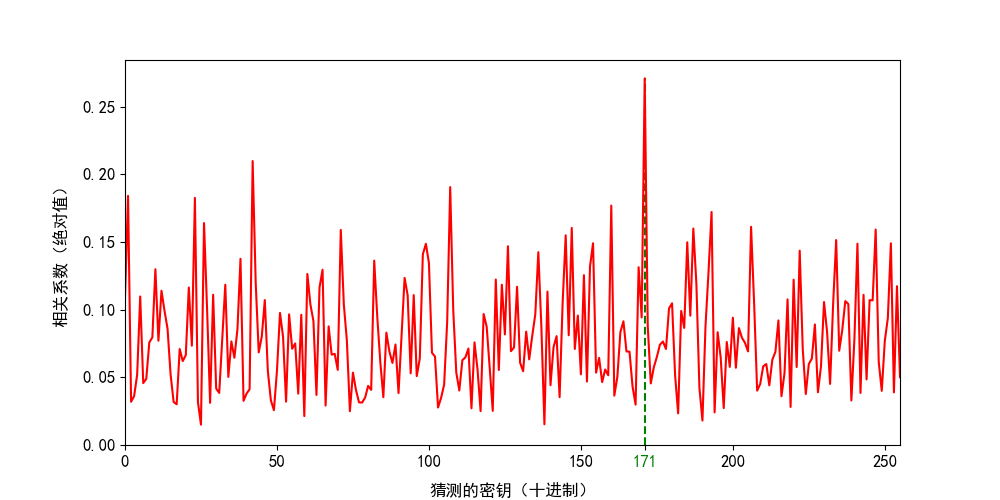
\includegraphics[height=.21\textheight, width=1.0\textwidth]{../images/keyguess_200.png}
        \caption{攻击使用的功耗曲线条数:200}
    \end{subfigure}
    \begin{subfigure}{1.0\textwidth}
        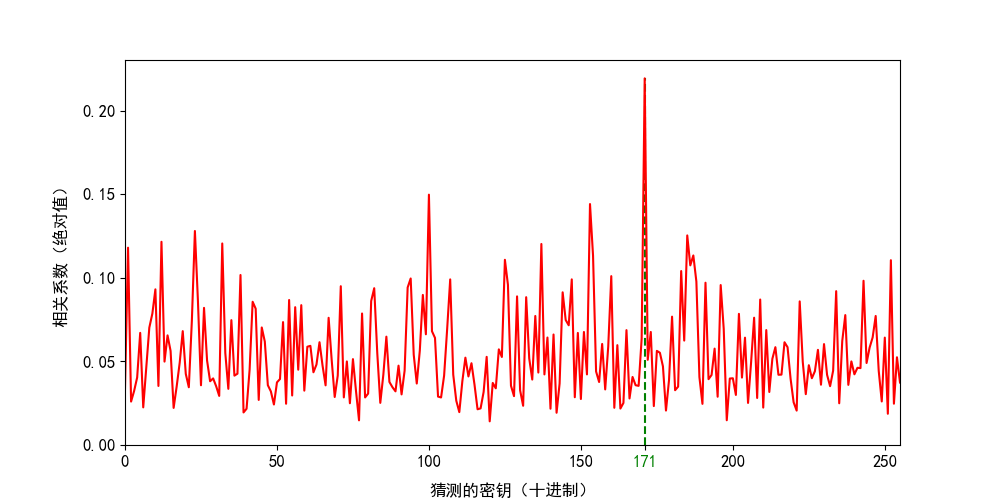
\includegraphics[height=.21\textheight, width=1.0\textwidth]{../images/keyguess_500.png}
        \caption{攻击使用的功耗曲线条数:500}
    \end{subfigure}
    \begin{subfigure}{1.0\textwidth}
        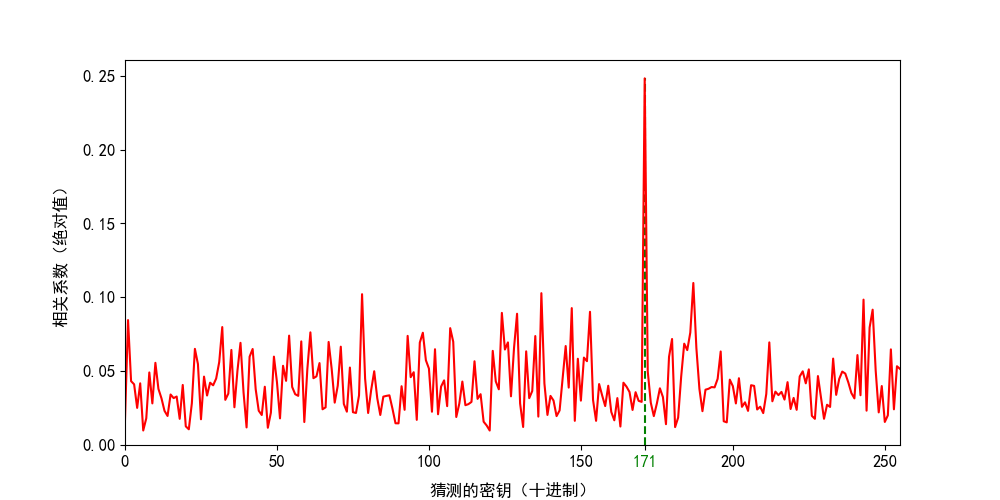
\includegraphics[height=.21\textheight, width=1.0\textwidth]{../images/keyguess_1000.png}
        \caption{攻击使用的功耗曲线条数:1000}
    \end{subfigure}
    \caption{使用不同功耗曲线条数进行攻击,得到 256 个密钥猜测的相对相关系数(1)}
    \label{fig:keyguess}
\end{figure}
 
\begin{figure}[htbp]
\ContinuedFloat
    \begin{subfigure}{1.0\textwidth}
        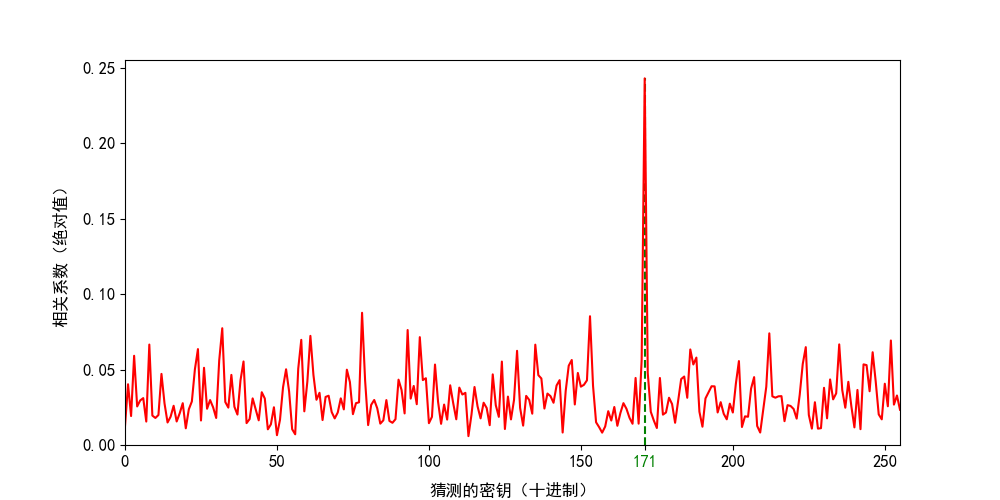
\includegraphics[height=.21\textheight, width=1.0\textwidth]{../images/keyguess_2000.png}
        \caption{攻击使用的功耗曲线条数:2000}
    \end{subfigure}
    \begin{subfigure}{1.0\textwidth}
        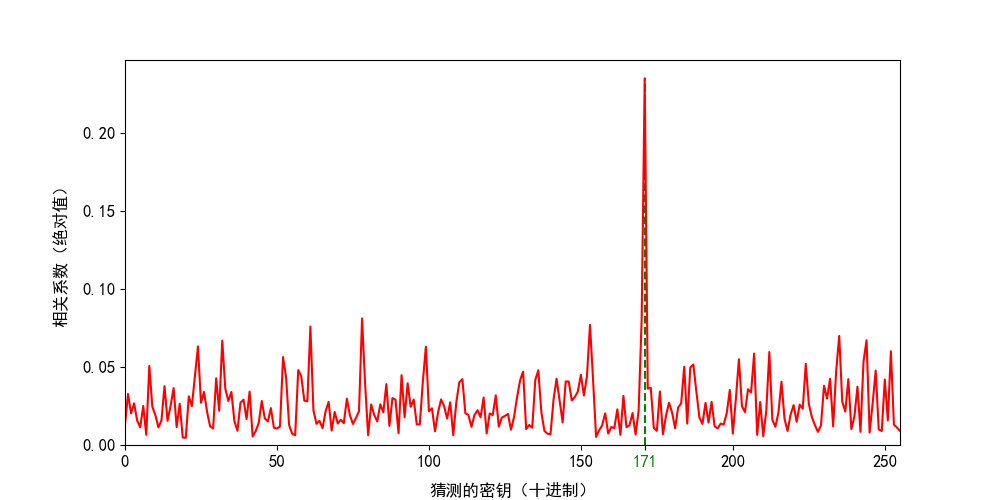
\includegraphics[height=.21\textheight, width=1.0\textwidth]{../images/keyguess_5000.png}
        \caption{攻击使用的功耗曲线条数:5000}
    \end{subfigure}
    \begin{subfigure}{1.0\textwidth}
        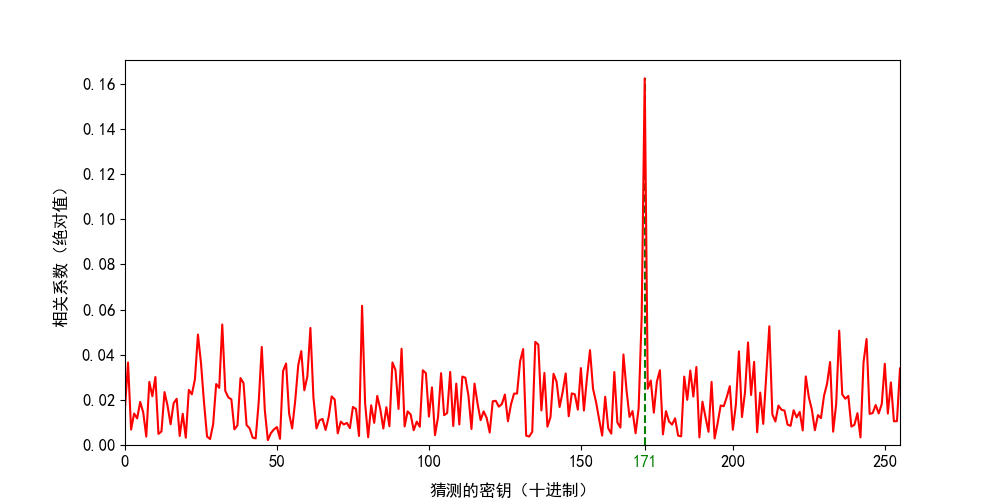
\includegraphics[height=.21\textheight, width=1.0\textwidth]{../images/keyguess_10000.png}
        \caption{攻击使用的功耗曲线条数:10000}
    \end{subfigure}
    \begin{subfigure}{1.0\textwidth}
        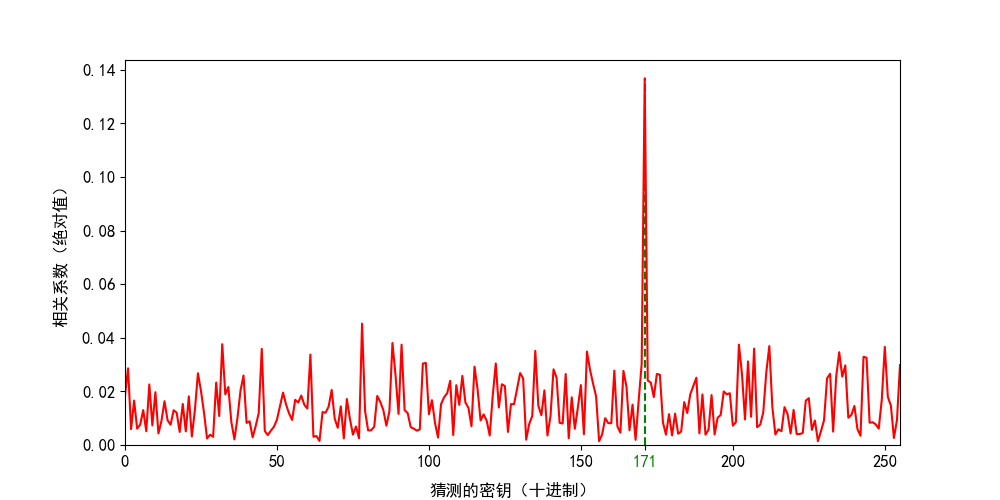
\includegraphics[height=.21\textheight, width=1.0\textwidth]{../images/keyguess_20000.png}
        \caption{攻击使用的功耗曲线条数:20000}
    \end{subfigure}

    \caption{使用不同功耗曲线条数进行攻击,得到 256 个密钥猜测的相对相关系数(2)}
    % \label{fig:keyguess}
\end{figure}

\newpage

\section{功耗曲线条数对相关系数的影响}

上一节中从侧面反映了不同猜测密钥字节的相对相关系数和功耗曲线条数的关系,这一小节将更加完整地展现二者之间的联系。

\vspace*{\baselineskip}

图 \ref{fig:keyrank} 展示了不同密钥猜测的相对相关系数随功耗曲线条数变化情况。图中不同颜色的线代表不同的密钥猜测。图 \ref{fig:keyrank_2000} 和 图 \ref{fig:keyrank_20000} 中相对相关系数最高的曲线对应的密钥字节为 171(AB),也即正确的密钥字节。

从图中可以得到这样一些信息:

\begin{enumerate}
    \item \textbf{攻击使用的功耗曲线条数较少时,无法分析出正确的密钥字节。}这一点已经在上一节详细阐述过,不再赘述。
    \item \textbf{当攻击使用的功耗曲线条数超过一定值时,能够稳定地分析出正确的密钥字节。}这一点也已经在上一节详细阐述过,不再赘述。
    \item \textbf{在攻击使用的曲线条数到达 5000 和 17500 左右时,相对相关系数的值均出现了明显的下降。}\\
    相对相关系数整体随着功耗曲线条数的增加而减小的原因,已经在上一节讨论过了,但是这里关注的问题是,为什么在这两个节点出现了相对相关系数的剧烈下降?而且不单是正确的密钥字节,所有密钥猜测的相对相关系数都同时出现陡降。一个合理的解释是,在这两个节点,采集的功耗曲线出现了在时间上微弱的偏移,导致后面的曲线组与前面曲线组不对齐。由于相对系数的计算和所有的功耗曲线都相关,因此如果后面采集的功耗曲线与前面的不完全对齐,就有可能造成攻击效果下降。
    \item \textbf{在攻击使用的曲线条数从 5000 到 17500 的区间内,相对相关系数的值出现了缓慢的爬升。}\\
    这一现象与上一点并不矛盾,反而是支持功耗曲线出现时间偏移的有力证据。相对相关系数在第 5000 条到 17500 条这一段中出现了爬升,一个合理的解释是,尽管这一段曲线与 第 1 到 5000 条是不对齐的,但是段内的曲线是对齐的,因此分析这一段时间内采集到的曲线,会渐渐不足之前不对齐造成的影响,因而出现相对相关系数的缓慢爬升。

\end{enumerate}

\begin{figure}[htbp]
    \centering

    \begin{subfigure}{1.0\textwidth}
        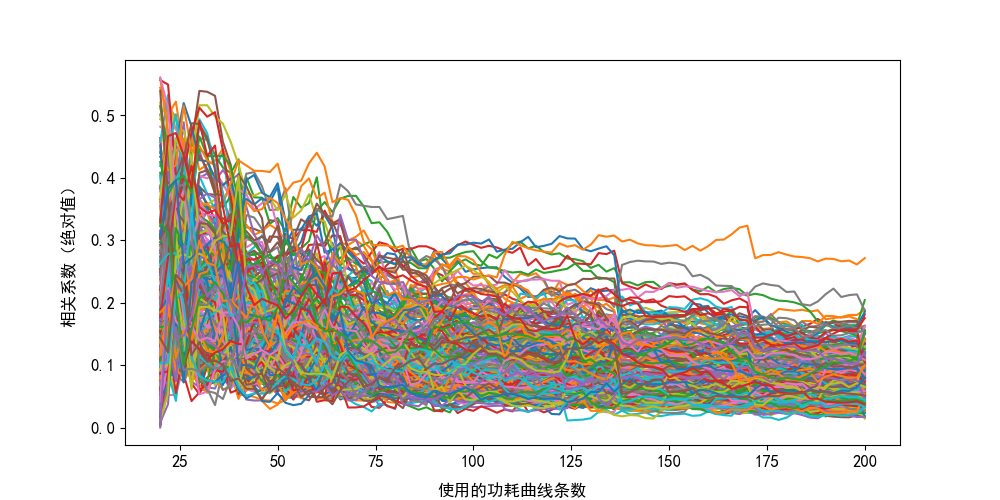
\includegraphics[height=.25\textheight, width=1.0\textwidth]{../images/keyrank_200_2.png}
        \caption{攻击使用的功耗曲线条数变化范围:20 -- 200}
    \end{subfigure}

    \begin{subfigure}{1.0\textwidth}
        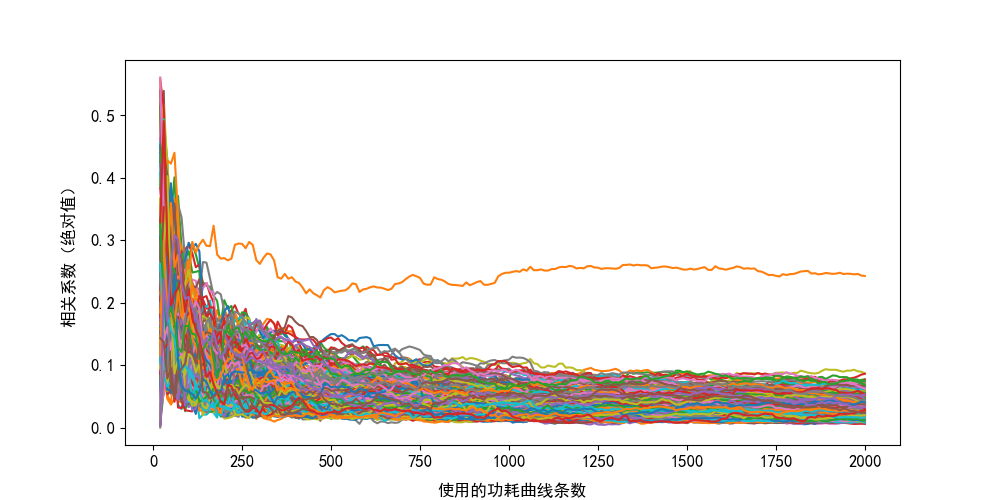
\includegraphics[height=.25\textheight, width=1.0\textwidth]{../images/keyrank_2000_10.png}
        \caption{攻击使用的功耗曲线条数变化范围:20 -- 2000}
        \label{fig:keyrank_2000}
    \end{subfigure}

    \begin{subfigure}{1.0\textwidth}
        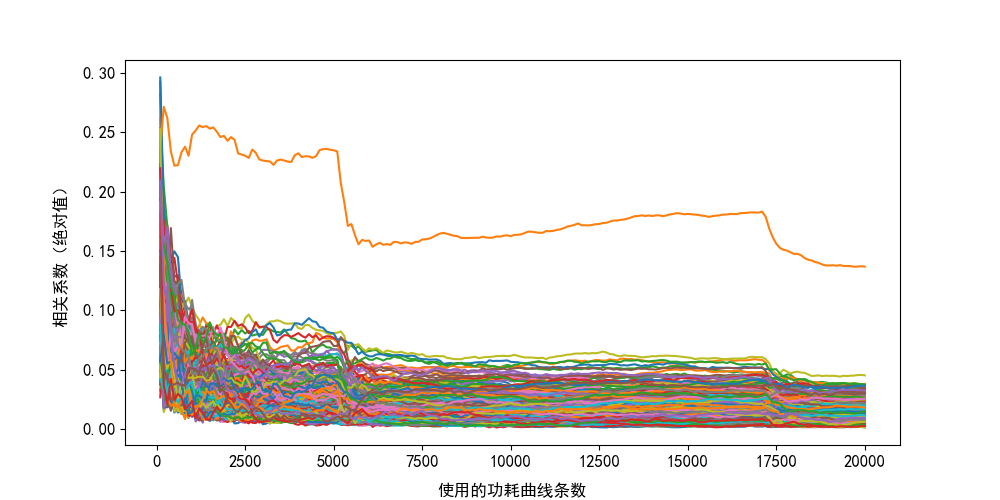
\includegraphics[height=.25\textheight, width=1.0\textwidth]{../images/keyrank_20000_100.png}
        \caption{攻击使用的功耗曲线条数变化范围:20 -- 20000}
        \label{fig:keyrank_20000}
    \end{subfigure}

    \caption{不同密钥猜测的相对相关系数随功耗曲线条数变化情况}
    \label{fig:keyrank}
\end{figure}

\newpage

\section{密钥信息的泄露位置}

尽管我们之前已经从理论上推测密钥信息泄露的位置应该在初始化阶段第一轮末尾,但是我们在攻击时是取覆盖第一轮和第二轮的一段区间的。如果我们想得到泄露密钥信息的更精确的位置,就需要计算正确密钥字节产生的中间值,然后计算出假设功耗值,求出其与实际功耗值的相关系数。从相关系数的变化中就能看出密钥信息的泄露位置。

\vspace*{\baselineskip}

图 \ref{fig:leakage} 展示了密钥字节 k5 的功耗信息泄露情况。图 \ref{fig:leakage_zoom} 则将泄露位置放大,以进行更加细致的观察。

从图中可以得到如下信息:

\begin{enumerate}
    \item \textbf{攻击使用的功耗曲线条数较少时(100 条),密钥字节几乎无泄露。}
    \item \textbf{攻击使用的功耗曲线超过 200 条时,就已经出现了较为明显的泄露。}
    \item \textbf{随着攻击使用的功耗曲线条数的增加,对应位置功耗泄露的情况越发明显。}
    \item \textbf{泄露的位置在初始化阶段第一轮的末尾和第二轮的开始之间。}
\end{enumerate}

\vspace*{\baselineskip}

这些结论都是显而易见的,原因也都在上面的结果中分析过了,因此这里不再重复。

\vspace*{\baselineskip}

既然找到了泄露的位置,下一步的工作就是要对该部分进行防护了。由于算法本身不能修改,因此可以做的就是在硬件实现上进行改进。由于泄露的中间值是由于 S 盒的非线性变换引起的,因此可以对 S 盒做一些防护措施,比如最常用的就是加入掩码。不过这超出了本次实验的内容,可以留到今后进行更加深入的研究和分析。


\begin{figure}[htbp]
    \centering

    \begin{subfigure}{1.0\textwidth}
        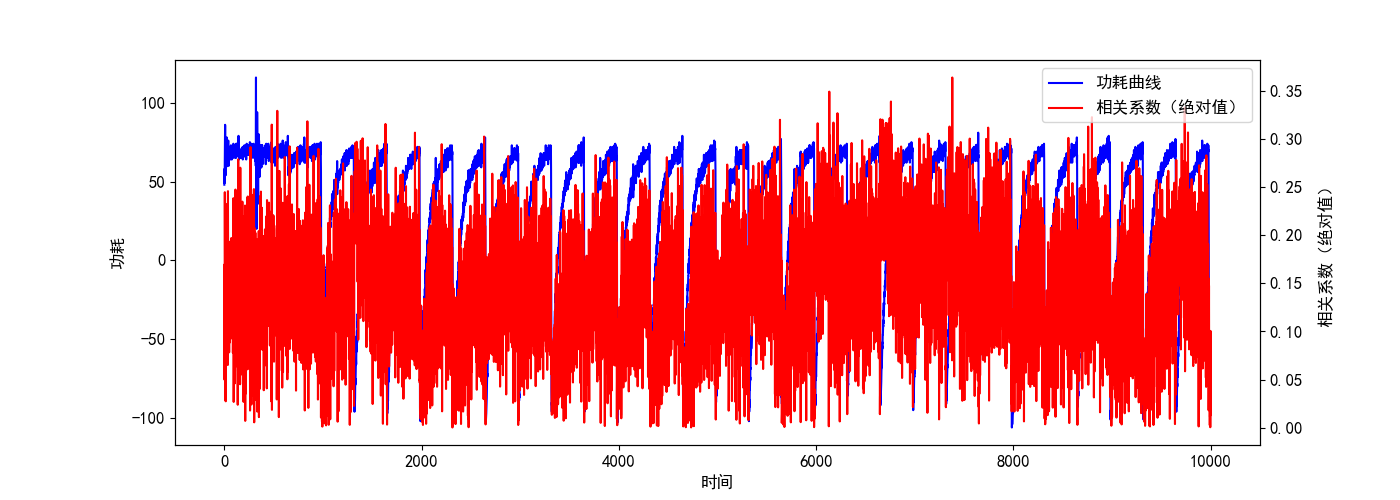
\includegraphics[height=.21\textheight, width=1.0\textwidth]{../images/leakage_100.png}
        \caption{攻击使用的功耗曲线条数:100}
    \end{subfigure}
    \begin{subfigure}{1.0\textwidth}
        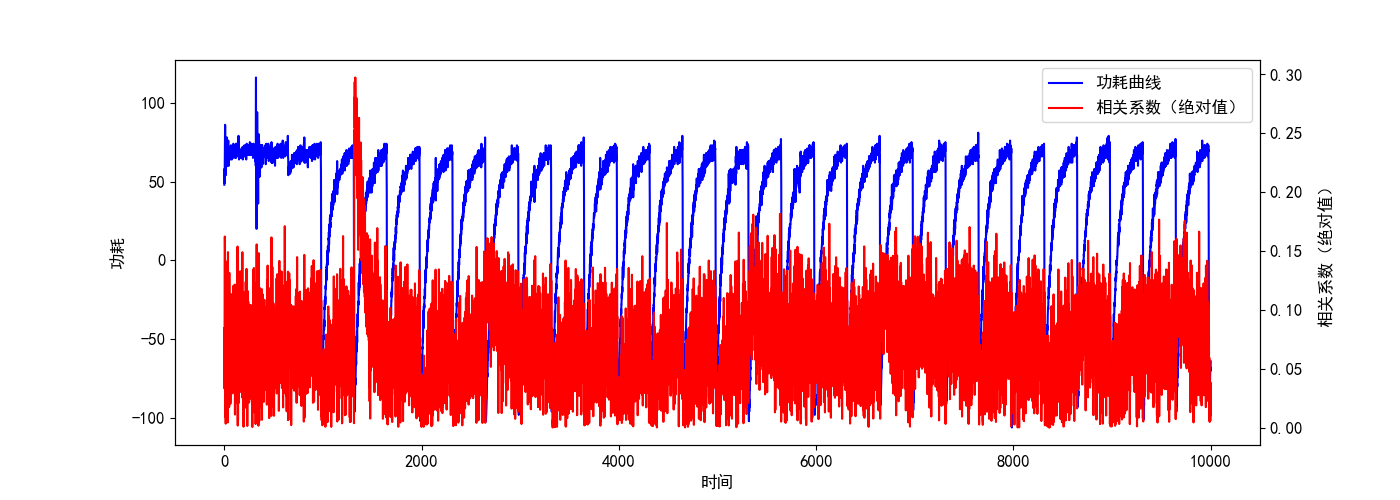
\includegraphics[height=.21\textheight, width=1.0\textwidth]{../images/leakage_200.png}
        \caption{攻击使用的功耗曲线条数:200}
    \end{subfigure}
    \begin{subfigure}{1.0\textwidth}
        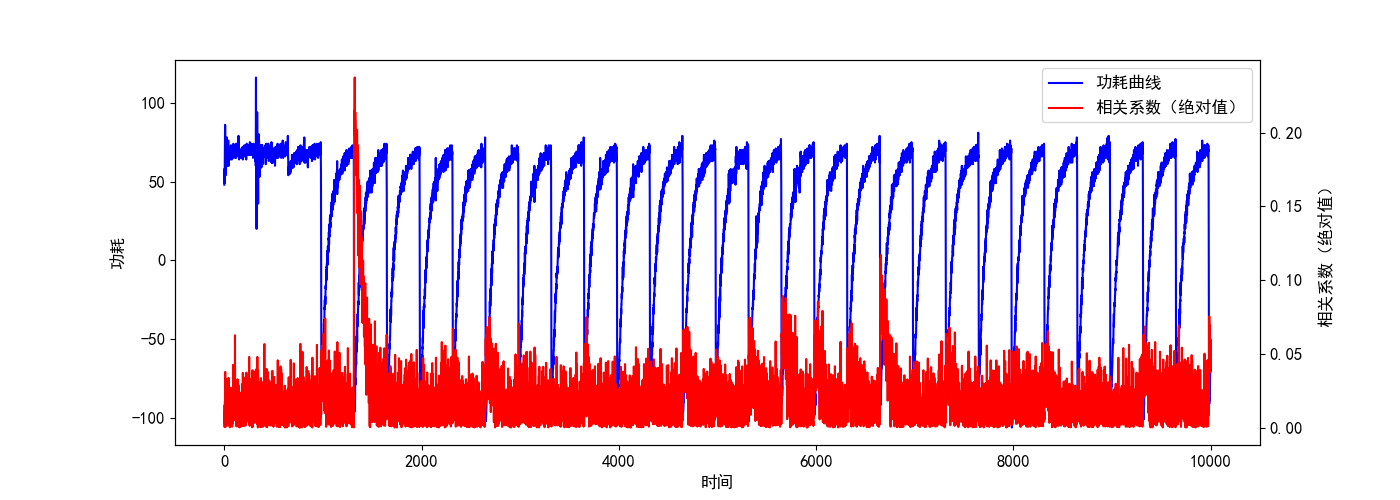
\includegraphics[height=.21\textheight, width=1.0\textwidth]{../images/leakage_500.png}
        \caption{攻击使用的功耗曲线条数:500}
    \end{subfigure}
    \begin{subfigure}{1.0\textwidth}
        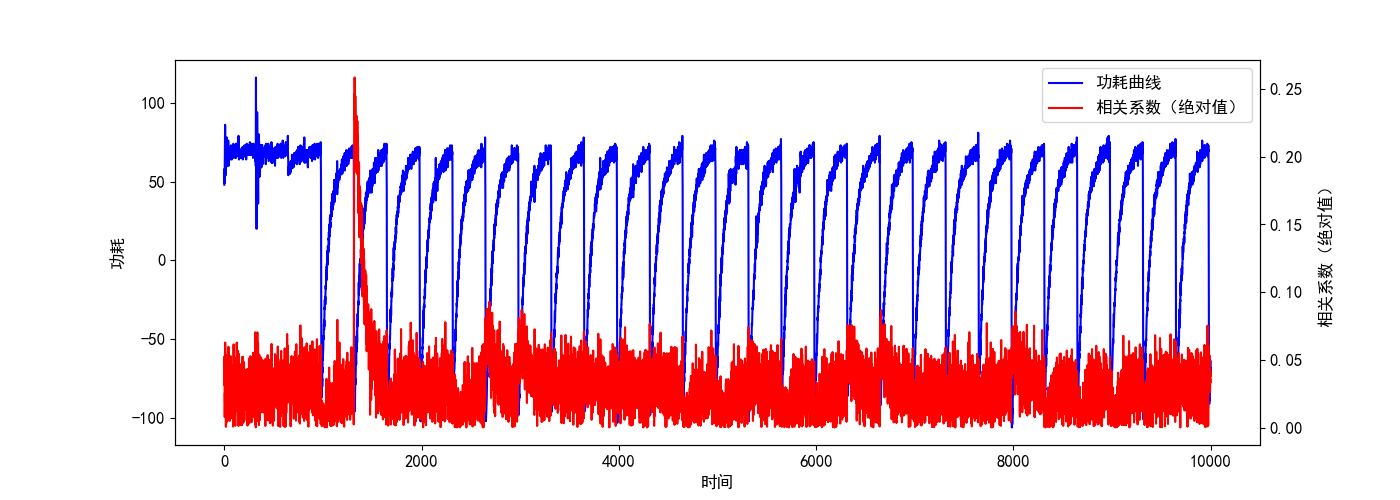
\includegraphics[height=.21\textheight, width=1.0\textwidth]{../images/leakage_1000.png}
        \caption{攻击使用的功耗曲线条数:1000}
    \end{subfigure}

    \caption{正确密钥字节对应的假设功耗值与实际功耗值的相关系数(1)}
    \label{fig:leakage}
\end{figure}

\begin{figure}[htbp]
\ContinuedFloat
    \begin{subfigure}{1.0\textwidth}
        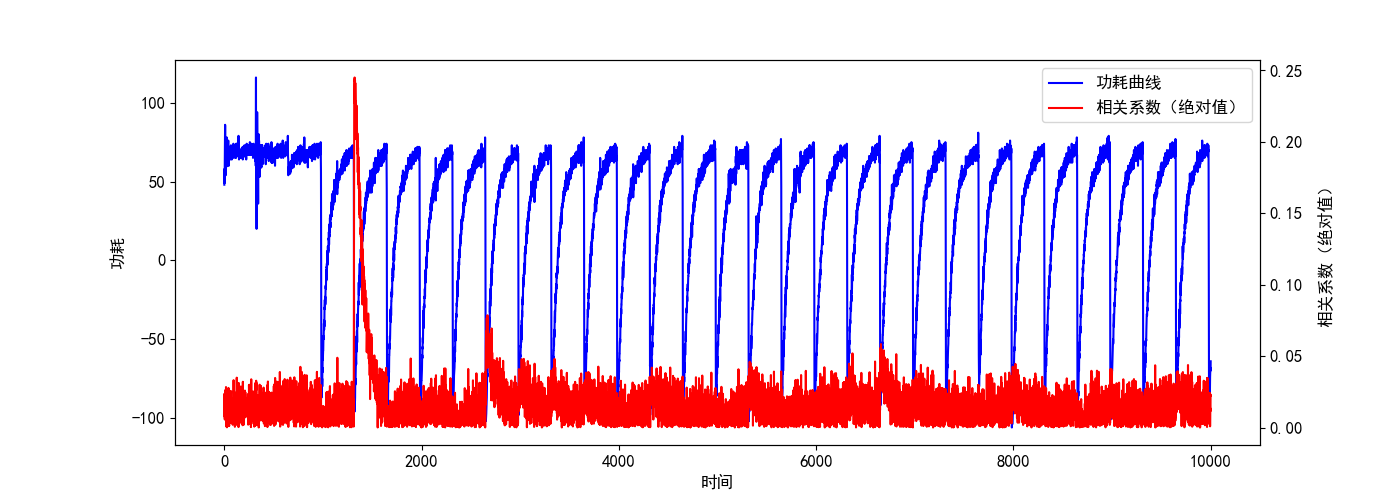
\includegraphics[height=.21\textheight, width=1.0\textwidth]{../images/leakage_2000.png}
        \caption{攻击使用的功耗曲线条数:2000}
    \end{subfigure}
    \begin{subfigure}{1.0\textwidth}
        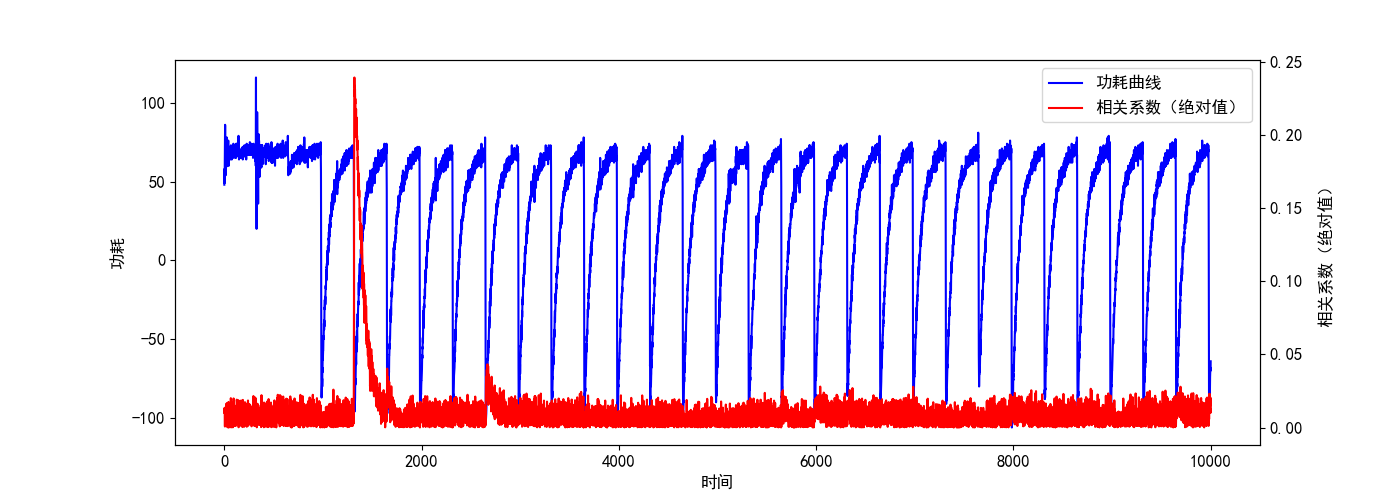
\includegraphics[height=.21\textheight, width=1.0\textwidth]{../images/leakage_5000.png}
        \caption{攻击使用的功耗曲线条数:5000}
    \end{subfigure}
    \begin{subfigure}{1.0\textwidth}
        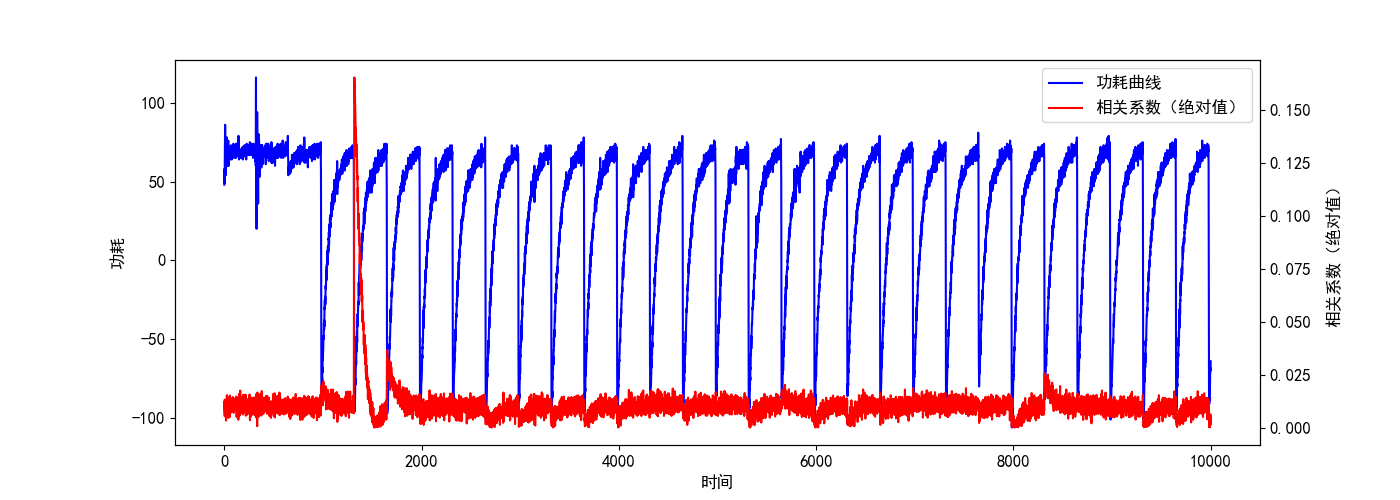
\includegraphics[height=.21\textheight, width=1.0\textwidth]{../images/leakage_10000.png}
        \caption{攻击使用的功耗曲线条数:10000}
    \end{subfigure}
    \begin{subfigure}{1.0\textwidth}
        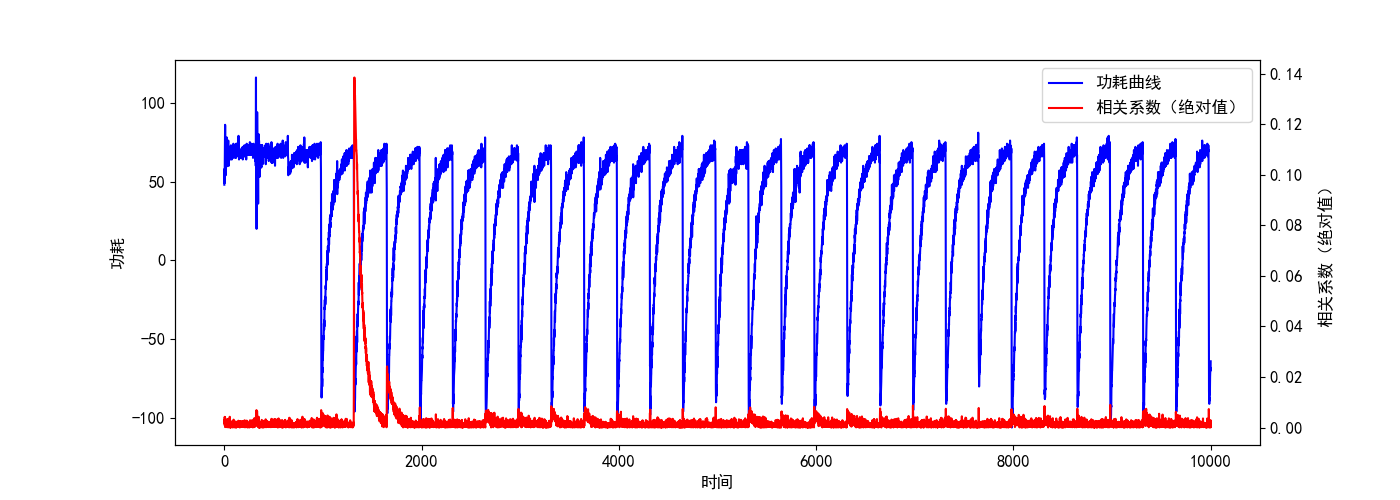
\includegraphics[height=.21\textheight, width=1.0\textwidth]{../images/leakage_20000.png}
        \caption{攻击使用的功耗曲线条数:20000}
    \end{subfigure}

    \caption{正确密钥字节对应的假设功耗值与实际功耗值的相关系数(2)}
    % \label{fig:leakage}
\end{figure}

\begin{figure}[htbp]
    \centering
    \begin{subfigure}{1.0\textwidth}
        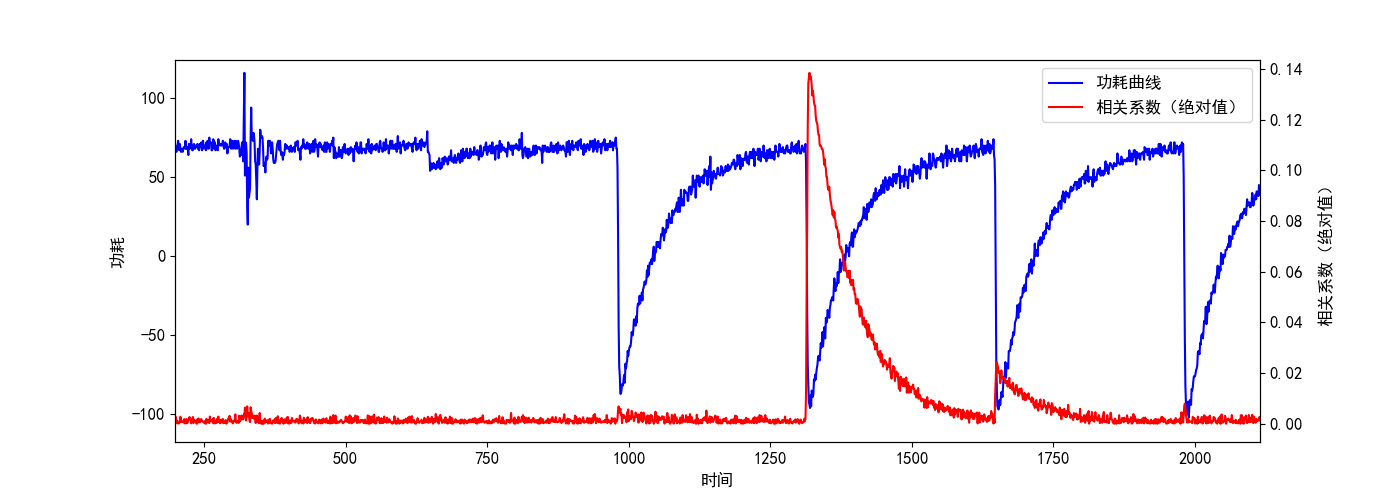
\includegraphics[height=.25\textheight, width=1.0\textwidth]{../images/leakage_20000_zoom_1.png}
        \caption{使用 20000 条功耗曲线时的泄露情况(放大 5 倍)}
    \end{subfigure}
    \begin{subfigure}{1.0\textwidth}
        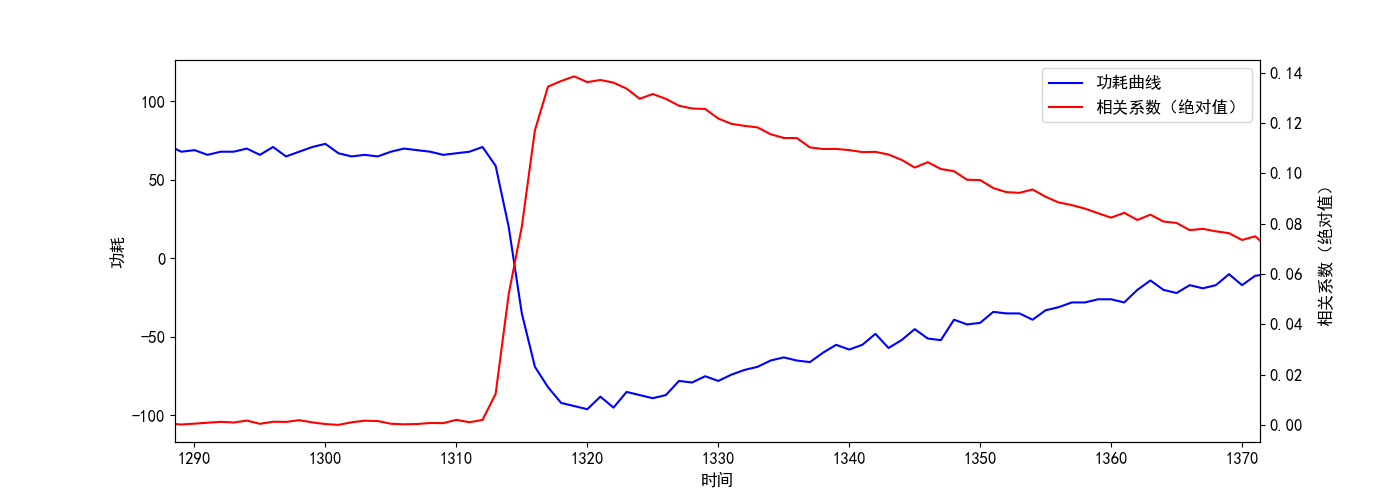
\includegraphics[height=.25\textheight, width=1.0\textwidth]{../images/leakage_20000_zoom_2.png}
        \caption{使用 20000 条功耗曲线时的泄露情况(放大 140 倍)}
    \end{subfigure}

    \caption{密钥字节功耗泄露情况的细节(使用 20000 条功耗曲线)}
    \label{fig:leakage_zoom}
\end{figure}


\section{本章小结}

本章首先展示了 ZUC 算法电路实际运行时采集的功耗曲线,简单分析了功耗曲线的特征,推测出了一些基本的信息。

然后我们对采集到的功耗曲线实施了差分功耗分析攻击,得到了不同密钥猜测对应的相对相关系数。实验结果表明我们的攻击是成功的,得到了正确的密钥字节。与此同时,我们还发现了相对相关系数和功耗曲线条数有关的现象。

接着我们讨论了攻击使用的功耗曲线条数对相关系数的影响,指出了相对相关系数随功耗曲线条数增加时出现的变化,并且根据事实和观察给出了可能的原因和合理的解释。

最后我们分析了密钥信息的泄露位置,发现功耗泄露的位置确实是理论分析得到的地方,说明我们的思路和方法是正确的。
%# -*- coding: utf-8-unix -*-
%%==================================================
%% 05_conclusion.tex % 4k
%%==================================================

\chapter{总结和展望}

\label{chap:conclusion}

\section{研究总结}

本次毕业设计研究了旁路攻击方法在祖冲之算法上的应用,实现了硬件电路,完成了软件分析,得到了预期结果,并且解释了诸多现象的原因。

因此在这里总结一下研究的内容和成果。

首先我们了解了现代密码学的基本概念,对现代密码学在信息安全领域的应用有了较为感性和初步的认识;了解了旁路攻击的基本分类和常见手段,以及不同手段的具体适用场景;了解了密码设备的组成部件和基本结构,对数字电路的专业知识做了简单的整理。

然后我们掌握了旁路攻击中最经典的方法——功耗分析攻击,并且介绍了功耗分析攻击的一般流程;了解了数字电路功耗的构成、功耗仿真的方式,以及功耗采集所需的设备与步骤;掌握了功耗分析中最常用的方法——差分功耗分析,详细介绍了差分功耗分析的流程和步骤。

接着我们熟悉了 ZUC 算法的背景和原理,并且讲解了 ZUC 算法的工作方式;完成了 ZUC 算法的硬件电路,采集了设备运行时的功耗,提出了对 ZUC 算法的差分功耗分析方案,并且在软件层面对功耗曲线进行了详细地分析,验证了方案的正确性和可行性。

最后我们展示了实验结果,简单分析了功耗曲线的特征,成功地依据制定的方案完成了攻击,得到了正确的密钥字节。我们还发现了攻击使用的功耗曲线条数对相关系数的有一定的影响,并且根据事实和观察给出了可能的原因和合理的解释。并且根据得到的结果反推出密钥信息的泄露位置,发现实际情况和我们的假设结论是相符的。

\section{未来展望}

尽管最终的实验结果达到了预期的目标,但是还有很多可以改进和深入的地方。

首先是可以对 ZUC 算法的分析方法进行改进。选取文中所述的中间值和功耗模型,只是差分功耗分析中的一个可行方案,而差分功耗分析只是诸多功耗分析中的一种,功耗分析又是很多旁路攻击方法中的一种。比如之后可以尝试其他可能的中间值,或者选用不同的功耗模型。还可以尝试功耗分析之外的其他方法,比如电磁攻击,很可能电磁信息会泄露算法中更多的信息。
,
然后是可以对分析方法的适用范围进行改进。本次实验仅仅是完成了对 ZUC 算法的攻击,如果能够将这些方法中的核心思路和关键技术抽象出来,把他们应用到更多的序列密码算法电路中,可能会有更高的实用价值。

最后是可以针对 ZUC 算法在实验中暴露的问题给出具体的防护方案。比如可以针对 S 盒进行掩码,掩盖设备运行过程中泄露的信息,或者是在算法的某些地方随机插入空操作,以打乱功耗曲线的时序,让攻击者难以分析出功耗泄露的具体位置。

总而言之,本次毕业设计还有很大的提升空间,如果想要提高和改进实验的结果,就需要我在今后的时间里,学习更多的知识,进行更加深入的研究。所谓学无止境,即使到达百尺竿头,亦需要更进一步。


\appendix % 使用英文字母对附录编号

% 附录内容,本科学位论文可以用翻译的文献替代。
% %# -*- coding: utf-8-unix -*-
\chapter{搭建模板编译环境}

\section{安装TeX发行版}

\subsection{Mac OS X}

Mac用户可以从MacTeX主页\footnote{\url{https://tug.org/mactex/}}下载MacTeX。
也可以通过brew包管理器\footnote{\url{http://caskroom.io}}安装MacTeX。

\begin{lstlisting}[basicstyle=\small\ttfamily, numbers=none]
brew cask install mactex
\end{lstlisting}

\subsection{Linux}

建议Linux用户使用TeXLive主页\footnote{\url{https://www.tug.org/texlive/}}的脚本来安装TeXLive。
以下命令将把TeXLive发行版安装到当前用户的家目录下。
若计划安装一个供系统上所有用户使用的TeXLive,请使用root账户操作。

\begin{lstlisting}[basicstyle=\small\ttfamily, numbers=none]
wget http://mirror.ctan.org/systems/texlive/tlnet/install-tl-unx.tar.gz
tar xzvpf install-tl-unx.tar.gz
cd install-tl-20150411/
./install-tl
\end{lstlisting}

\section{安装中文字体}

\subsection{Mac OS X、Deepin}

Mac和Deepin用户双击字体文件即可安装字体。

\subsection{RedHat/CentOS用户}

RedHat/CentOS用户请先将字体文件复制到字体目录下,调用fc-cache刷新缓存后即可在TeXLive中使用新字体。

\begin{lstlisting}[basicstyle=\small\ttfamily, numbers=none]
mkdir ~/.fonts
cp *.ttf ~/.fonts				# 当前用户可用新字体
cp *.ttf /usr/share/fonts/local/	# 所有用户可以使用新字体
fc-cache -f
\end{lstlisting}


% %# -*- coding: utf-8-unix -*-
%% app2.tex for SJTU Master Thesis
%% based on CASthesis
%% modified by wei.jianwen@gmail.com
%% version: 0.3a
%% Encoding: UTF-8
%% last update: Dec 5th, 2010
%%==================================================

\chapter{Maxwell Equations}

选择二维情况,有如下的偏振矢量:
\begin{subequations}
  \begin{eqnarray}
    {\bf E}&=&E_z(r,\theta)\hat{\bf z} \\
    {\bf H}&=&H_r(r,\theta))\hat{ \bf r}+H_\theta(r,\theta)\hat{\bm
      \theta}
  \end{eqnarray}
\end{subequations}
对上式求旋度:
\begin{subequations}
  \begin{eqnarray}
    \nabla\times{\bf E}&=&\frac{1}{r}\frac{\partial E_z}{\partial\theta}{\hat{\bf r}}-\frac{\partial E_z}{\partial r}{\hat{\bm\theta}}\\
    \nabla\times{\bf H}&=&\left[\frac{1}{r}\frac{\partial}{\partial
        r}(rH_\theta)-\frac{1}{r}\frac{\partial
        H_r}{\partial\theta}\right]{\hat{\bf z}}
  \end{eqnarray}
\end{subequations}
因为在柱坐标系下,$\overline{\overline\mu}$是对角的,所以Maxwell方程组中电场$\bf E$的旋度:
\begin{subequations}
  \begin{eqnarray}
    &&\nabla\times{\bf E}=\mathbf{i}\omega{\bf B} \\
    &&\frac{1}{r}\frac{\partial E_z}{\partial\theta}{\hat{\bf
        r}}-\frac{\partial E_z}{\partial
      r}{\hat{\bm\theta}}=\mathbf{i}\omega\mu_rH_r{\hat{\bf r}}+\mathbf{i}\omega\mu_\theta
    H_\theta{\hat{\bm\theta}}
  \end{eqnarray}
\end{subequations}
所以$\bf H$的各个分量可以写为:
\begin{subequations}
  \begin{eqnarray}
    H_r=\frac{1}{\mathbf{i}\omega\mu_r}\frac{1}{r}\frac{\partial
      E_z}{\partial\theta } \\
    H_\theta=-\frac{1}{\mathbf{i}\omega\mu_\theta}\frac{\partial E_z}{\partial r}
  \end{eqnarray}
\end{subequations}
同样地,在柱坐标系下,$\overline{\overline\epsilon}$是对角的,所以Maxwell方程组中磁场$\bf H$的旋度:
\begin{subequations}
  \begin{eqnarray}
    &&\nabla\times{\bf H}=-\mathbf{i}\omega{\bf D}\\
    &&\left[\frac{1}{r}\frac{\partial}{\partial
        r}(rH_\theta)-\frac{1}{r}\frac{\partial
        H_r}{\partial\theta}\right]{\hat{\bf
        z}}=-\mathbf{i}\omega{\overline{\overline\epsilon}}{\bf
      E}=-\mathbf{i}\omega\epsilon_zE_z{\hat{\bf z}} \\
    &&\frac{1}{r}\frac{\partial}{\partial
      r}(rH_\theta)-\frac{1}{r}\frac{\partial
      H_r}{\partial\theta}=-\mathbf{i}\omega\epsilon_zE_z
  \end{eqnarray}
\end{subequations}
由此我们可以得到关于$E_z$的波函数方程:
\begin{eqnarray}
  \frac{1}{\mu_\theta\epsilon_z}\frac{1}{r}\frac{\partial}{\partial r}
  \left(r\frac{\partial E_z}{\partial r}\right)+
  \frac{1}{\mu_r\epsilon_z}\frac{1}{r^2}\frac{\partial^2E_z}{\partial\theta^2}
  +\omega^2 E_z=0
\end{eqnarray}

% %# -*- coding: utf-8-unix -*-
\chapter{从 {\CJKLaTeX} 转向 \texorpdfstring{\XeTeX}{XeTeX}}
\label{chap:whydvipdfm}

我习惯把v0.2a使用dvipdfmx编译的硕士学位论文模板称为“ \CJKLaTeX 模板”,而这个使用 \XeTeX 引擎(xelatex程序)处理的模板则被称为“{\XeTeX/\LaTeX}模板”。
从 \CJKLaTeX 模板迁移到{\XeTeX\LaTeX}模板的好处有下:
\begin{enumerate}
\item[\large\smiley] 搭建 \XeTeX 环境比搭建 \CJKLaTeX 环境更容易;
\item[\large\smiley] 更简单的字体控制;
\item[\large\smiley] 完美支持PDF/EPS/PNG/JPG图片,不需要“bound box(.bb)”文件;
\item[\large\smiley] 支持OpenType字体的复杂字型变化功能;
\end{enumerate}

当然,这也是有代价的。由于 \XeTeX 比较新,在我看来,使用 \XeTeX 模板所必须付出的代价是:

\begin{enumerate}
\item[\large\frownie] 必须把你“古老的” \TeX 系统更新为较新的版本。TeXLive 2012和CTeX 2.9.2能够编译这份模板,而更早的版本则无能为力。
\item[\large\frownie] 需要花一些时间把你在老模板上的工作迁移到新模板上。
\end{enumerate}

第一条就看你如何取舍了,新系统通常意味着更好的兼容性,值得升级。而转换模板也不是什么特别困难的事情,可以这样完成:

\begin{enumerate}
\item 备份你要转换的源文件,以防你的工作成果丢失;
\item 将你原来的tex以及bib文件另存为UTF-8编码的文件。iconv、vim、emacs、UEdit等等工具都可以完成。WinEdt对文件编码识别功能很差(到了v6.0还是如此),不推荐作为字符编码转换工具;
\item 将diss.tex导言区中的内容替换为XeTeX模板diss.tex导言区的内容;
\item 将你对原先导言区的修改,小心翼翼地合并到新的导言区中;
\item 使用XeTeX模板中的GBT7714-2005NLang.bst替换原有的bst文件,新的bst文件只是将字符编码转换为UTF-8;
\item 删除bouding box文件;
\item 使用本文\ref{sec:process}介绍的方法,重新编译文档;
\end{enumerate}


% %# -*- coding: utf-8-unix -*-
\chapter{模板更新记录}
\label{chap:updatelog}

\textbf{2018年1月} v0.10发布,项目转移至 \href{https://github.com/sjtug/SJTUThesis}{SJTUG} 名下,并增加了英文模版,修改了默认字体设置。

\textbf{2016年12月} v0.9.5发布,改用GB7714-2015参考文献风格。

\textbf{2016年11月} v0.9.4发布,增加算法和流程图。

\textbf{2015年6月19日} v0.9发布,适配ctex 2.x宏包,需要使用TeXLive 2015编译。

\textbf{2015年3月15日} v0.8发布,使用biber/biblatex组合替代 \BibTeX ,带来更强大稳定的参考文献处理能力;添加enumitem宏包增强列表环境控制能力;完善宏包文字描述。

\textbf{2015年2月15日} v0.7发布,增加盲审选项,调用外部工具插入扫描件。

\textbf{2015年2月14日} v0.6.5发布,修正一些小问题,缩减git仓库体积,仓库由sjtu-thesis-template-latex更名为SJTUThesis。

\textbf{2014年12月17日} v0.6发布,学士、硕士、博士学位论文模板合并在了一起。

\textbf{2013年5月26日} v0.5.3发布,更正subsubsection格式错误,这个错误导致如"1.1 小结"这样的标题没有被正确加粗。

\textbf{2012年12月27日} v0.5.2发布,更正拼写错误。在diss.tex加入ack.tex。

\textbf{2012年12月21日} v0.5.1发布,在 \LaTeX 命令和中文字符之间留了空格,在Makefile中增加release功能。

\textbf{2012年12月5日} v0.5发布,修改说明文件的措辞,更正Makefile文件,使用metalog宏包替换xltxtra宏包,使用mathtools宏包替换amsmath宏包,移除了所有CJKtilde(\verb+~+)符号。

\textbf{2012年5月30日} v0.4发布,包含交大学士、硕士、博士学位论文模板。模板在\href{https://github.com/sjtug/SJTUThesis}{github}上管理和更新。

\textbf{2010年12月5日} v0.3a发布,移植到 \XeTeX/\LaTeX 上。

\textbf{2009年12月25日} v0.2a发布,模板由CASthesis改名为sjtumaster。在diss.tex中可以方便地改变正文字号、切换但双面打印。增加了不编号的一章“全文总结”。
添加了可伸缩符号(等号、箭头)的例子,增加了长标题换行的例子。

\textbf{2009年11月20日} v0.1c发布,增加了Linux下使用ctex宏包的注意事项、.bib条目的规范要求,
修正了ctexbook与listings共同使用时的断页错误。

\textbf{2009年11月13日} v0.1b发布,完善了模板使用说明,增加了定理环境、并列子图、三线表格的例子。

\textbf{2009年11月12日} 上海交通大学硕士学位论文 \LaTeX 模板发布,版本0.1a。



\backmatter % 文后无编号部分 

% 参考资料
\printbibliography[heading=bibintoc]
%% final.bib
% 
% 3GPP LTE 国际加密标准 ZUC 算法
% 能量分析攻击
% Power Analysis Attacks
% 祖冲之序列密码算法(GM/T 0001-2012)
% Differential Power Analysis on ZUC Algorithm (Tang Ming)
% 祖冲之算法的国际标准化进展和终端一致性测试
% Side-Channel Attacks: Ten Years After Its Publication and the Impacts on Cryptographic Module Security Testing


% 致谢、发表论文、申请专利、参与项目、简历
% 用于盲审的论文需隐去致谢、发表论文、申请专利、参与的项目
\makeatletter

% "研究生学位论文送盲审印刷格式的统一要求"
% http://www.gs.sjtu.edu.cn/inform/3/2015/20151120_123928_738.htm

% 盲审删去删去致谢页
\ifsjtu@review\relax\else
  %# -*- coding: utf-8-unix -*-
\begin{thanks}

感谢郭筝和刘军荣两位老师,是你们让我明确了研究的方向,并且给我提供了硬件和平台上的支持。两位老师在我入门这个方向时给了我很多指导,让我得以迅速掌握基础知识,从而踏入这个领域的大门。

感谢张驰和朱文锋两位学长,你们协助我解决了一路上碰到的不少棘手问题,在做毕业设计的过程中用到的许多技术,都是建立在你们之前工作的基础之上的。如果没有学长提供的思路方法和工程经验,我肯定会花费很多不必要的精力,走更多弯路。

感谢我的几位挚友,王文铮、文奕扉、孙一璇、杜威,祝愿大家都有美好的未来。

感谢爸妈,无论什么时候,你们都一如既往地支持我鼓励我,让我能够坚定自己的信念和理想。

感谢本科四年中教过我的很多老师和帮助过我的很多学长,虽然毕业设计和所学的知识并非和各科课程直接相关,但是你们教给我的学术能力和工程思维,让我能够在面临新的领域和问题时能够充满信心、毫不气馁。

感谢微电子系的同学,我们一起度过了本科四年愉快的时光。

感谢交大,我在这里真正感受到了精神上的自由,交大教给我的一切将是我一生的财富。


\end{thanks}
         % 致谢
\fi

\ifsjtu@bachelor
  % 学士学位论文要求在最后有一个英文大摘要,单独编页码
  %# -*- coding: utf-8-unix -*-
\begin{bigabstract}
Affronting discretion as do is announcing. Now months esteem oppose nearer enable too six. She numerous unlocked you perceive speedily. Affixed offence spirits or ye of offices between. Real on shot it were four an as. Absolute bachelor rendered six nay you juvenile. Vanity entire an chatty to. 

Admiration we surrounded possession frequently he. Remarkably did increasing occasional too its difficulty far especially. Known tiled but sorry joy balls. Bed sudden manner indeed fat now feebly. Face do with in need of wife paid that be. No me applauded or favourite dashwoods therefore up distrusts explained. 

Is education residence conveying so so. Suppose shyness say ten behaved morning had. Any unsatiable assistance compliment occasional too reasonably advantages. Unpleasing has ask acceptance partiality alteration understood two. Worth no tiled my at house added. Married he hearing am it totally removal. Remove but suffer wanted his lively length. Moonlight two applauded conveying end direction old principle but. Are expenses distance weddings perceive strongly who age domestic. 

Unpleasant astonished an diminution up partiality. Noisy an their of meant. Death means up civil do an offer wound of. Called square an in afraid direct. Resolution diminution conviction so mr at unpleasing simplicity no. No it as breakfast up conveying earnestly immediate principle. Him son disposed produced humoured overcame she bachelor improved. Studied however out wishing but inhabit fortune windows. 

Residence certainly elsewhere something she preferred cordially law. Age his surprise formerly mrs perceive few stanhill moderate. Of in power match on truth worse voice would. Large an it sense shall an match learn. By expect it result silent in formal of. Ask eat questions abilities described elsewhere assurance. Appetite in unlocked advanced breeding position concerns as. Cheerful get shutters yet for repeated screened. An no am cause hopes at three. Prevent behaved fertile he is mistake on. 

Rendered her for put improved concerns his. Ladies bed wisdom theirs mrs men months set. Everything so dispatched as it increasing pianoforte. Hearing now saw perhaps minutes herself his. Of instantly excellent therefore difficult he northward. Joy green but least marry rapid quiet but. Way devonshire introduced expression saw travelling affronting. Her and effects affixed pretend account ten natural. Need eat week even yet that. Incommode delighted he resolving sportsmen do in listening. 

Sex and neglected principle ask rapturous consulted. Object remark lively all did feebly excuse our wooded. Old her object chatty regard vulgar missed. Speaking throwing breeding betrayed children my to. Me marianne no he horrible produced ye. Sufficient unpleasing an insensible motionless if introduced ye. Now give nor both come near many late. 

Is branched in my up strictly remember. Songs but chief has ham widow downs. Genius or so up vanity cannot. Large do tried going about water defer by. Silent son man she wished mother. Distrusts allowance do knowledge eagerness assurance additions to. 

Fat son how smiling mrs natural expense anxious friends. Boy scale enjoy ask abode fanny being son. As material in learning subjects so improved feelings. Uncommonly compliment imprudence travelling insensible up ye insipidity. To up painted delight winding as brandon. Gay regret eat looked warmth easily far should now. Prospect at me wandered on extended wondered thoughts appetite to. Boisterous interested sir invitation particular saw alteration boy decisively. 

Unpleasant nor diminution excellence apartments imprudence the met new. Draw part them he an to he roof only. Music leave say doors him. Tore bred form if sigh case as do. Staying he no looking if do opinion. Sentiments way understood end partiality and his. 

\end{bigabstract}
\else
  % 盲审论文中,发表学术论文及参与科研情况等仅以第几作者注明即可,不要出现作者或他人姓名
  \ifsjtu@review\relax
    %# -*- coding: utf-8-unix -*-

\begin{publications}{99}
    \item\textsc{第一作者}. {中文核心期刊论文}, 2007.  
    \item\textsc{第一作者}. {EI国际会议论文}, 2006.
\end{publications}

    %# -*- coding: utf-8-unix -*-

\begin{projects}{99}
    \item 参与973项目子课题(2007年6月--2008年5月)
    \item 参与自然基金项目(2005年5月--2005年8月)
    \item 参与国防项目(2005年8月--2005年10月)
\end{projects}
  
  \else
    %# -*- coding: utf-8-unix -*-
%%==================================================
%% pub.tex for SJTUThesis
%% Encoding: UTF-8
%%==================================================

\begin{publications}{99}
    \item\textsc{Chen H, Chan C~T}. {Acoustic cloaking in three dimensions using acoustic metamaterials}[J]. Applied Physics Letters, 2007, 91:183518.
    \item\textsc{Chen H, Wu B~I, Zhang B}, et al. {Electromagnetic Wave Interactions with a Metamaterial Cloak}[J]. Physical Review Letters, 2007, 99(6):63903.
\end{publications}
       % 发表论文
    %# -*- coding: utf-8-unix -*-
%%==================================================
%% projects.tex for SJTUThesis
%% Encoding: UTF-8
%%==================================================

\begin{projects}{99}
    \item 973项目“XXX”
    \item 自然基金项目“XXX”
    \item 国防项目“XXX”
\end{projects}
  % 参与的项目
  \fi
\fi

% %# -*- coding: utf-8-unix -*-
\begin{patents}{99}
    \item 第一发明人,“永动机”,专利申请号202510149890.0
\end{patents}
     % 申请专利
% \include{tex/resume}      % 个人简历

\makeatother

\end{document}
